% template adapted from https://github.com/jgm/pandoc-templates/blob/master/default.latex
%%%%%%%%%%%%%%%%%%%%%%%%%%%%%%%%%%%%%%%%%%%%%%%%%%%%%%%%%%%%%%%%%%%%%%%%%%%%%%%%%%%%%%%%%

% Options for packages loaded elsewhere
\PassOptionsToPackage{unicode=true}{hyperref}
\PassOptionsToPackage{hyphens}{url}
\PassOptionsToPackage{dvipsnames,svgnames*,x11names*}{xcolor}


\documentclass[
  11pt,
  french,
  a4paper,
  extrafontsizes,onecolumn,openright
  ]{memoir}

% Font family: lmodern by default
\usepackage{lmodern}

% Double (or whatever) spacing

\usepackage{amssymb, amsmath}
\usepackage{ifxetex,ifluatex}

% mathspec: arbitrary math fonts
\usepackage{unicode-math}
\defaultfontfeatures{Ligatures=TeX,Scale=MatchLowercase}

% More font families
% Main font
% Specific sanserif font
% Specific monotype font
% Specific math font
% Chinese, Japanese, Corean fonts

% Use upquote if available, for straight quotes in verbatim environments
\IfFileExists{upquote.sty}{\usepackage{upquote}}{}
% Use microtype if available
\IfFileExists{microtype.sty}{%
\usepackage[]{microtype}
\UseMicrotypeSet[protrusion]{basicmath} % disable protrusion for tt fonts
}{}

% Verbatim in note

\usepackage{xcolor}


% Geometry package

% Listings package


\usepackage{color}
\usepackage{fancyvrb}
\newcommand{\VerbBar}{|}
\newcommand{\VERB}{\Verb[commandchars=\\\{\}]}
\DefineVerbatimEnvironment{Highlighting}{Verbatim}{commandchars=\\\{\}}
% Add ',fontsize=\small' for more characters per line
\usepackage{framed}
\definecolor{shadecolor}{RGB}{248,248,248}
\newenvironment{Shaded}{\begin{snugshade}}{\end{snugshade}}
\newcommand{\AlertTok}[1]{\textcolor[rgb]{0.94,0.16,0.16}{#1}}
\newcommand{\AnnotationTok}[1]{\textcolor[rgb]{0.56,0.35,0.01}{\textbf{\textit{#1}}}}
\newcommand{\AttributeTok}[1]{\textcolor[rgb]{0.77,0.63,0.00}{#1}}
\newcommand{\BaseNTok}[1]{\textcolor[rgb]{0.00,0.00,0.81}{#1}}
\newcommand{\BuiltInTok}[1]{#1}
\newcommand{\CharTok}[1]{\textcolor[rgb]{0.31,0.60,0.02}{#1}}
\newcommand{\CommentTok}[1]{\textcolor[rgb]{0.56,0.35,0.01}{\textit{#1}}}
\newcommand{\CommentVarTok}[1]{\textcolor[rgb]{0.56,0.35,0.01}{\textbf{\textit{#1}}}}
\newcommand{\ConstantTok}[1]{\textcolor[rgb]{0.00,0.00,0.00}{#1}}
\newcommand{\ControlFlowTok}[1]{\textcolor[rgb]{0.13,0.29,0.53}{\textbf{#1}}}
\newcommand{\DataTypeTok}[1]{\textcolor[rgb]{0.13,0.29,0.53}{#1}}
\newcommand{\DecValTok}[1]{\textcolor[rgb]{0.00,0.00,0.81}{#1}}
\newcommand{\DocumentationTok}[1]{\textcolor[rgb]{0.56,0.35,0.01}{\textbf{\textit{#1}}}}
\newcommand{\ErrorTok}[1]{\textcolor[rgb]{0.64,0.00,0.00}{\textbf{#1}}}
\newcommand{\ExtensionTok}[1]{#1}
\newcommand{\FloatTok}[1]{\textcolor[rgb]{0.00,0.00,0.81}{#1}}
\newcommand{\FunctionTok}[1]{\textcolor[rgb]{0.00,0.00,0.00}{#1}}
\newcommand{\ImportTok}[1]{#1}
\newcommand{\InformationTok}[1]{\textcolor[rgb]{0.56,0.35,0.01}{\textbf{\textit{#1}}}}
\newcommand{\KeywordTok}[1]{\textcolor[rgb]{0.13,0.29,0.53}{\textbf{#1}}}
\newcommand{\NormalTok}[1]{#1}
\newcommand{\OperatorTok}[1]{\textcolor[rgb]{0.81,0.36,0.00}{\textbf{#1}}}
\newcommand{\OtherTok}[1]{\textcolor[rgb]{0.56,0.35,0.01}{#1}}
\newcommand{\PreprocessorTok}[1]{\textcolor[rgb]{0.56,0.35,0.01}{\textit{#1}}}
\newcommand{\RegionMarkerTok}[1]{#1}
\newcommand{\SpecialCharTok}[1]{\textcolor[rgb]{0.00,0.00,0.00}{#1}}
\newcommand{\SpecialStringTok}[1]{\textcolor[rgb]{0.31,0.60,0.02}{#1}}
\newcommand{\StringTok}[1]{\textcolor[rgb]{0.31,0.60,0.02}{#1}}
\newcommand{\VariableTok}[1]{\textcolor[rgb]{0.00,0.00,0.00}{#1}}
\newcommand{\VerbatimStringTok}[1]{\textcolor[rgb]{0.31,0.60,0.02}{#1}}
\newcommand{\WarningTok}[1]{\textcolor[rgb]{0.56,0.35,0.01}{\textbf{\textit{#1}}}}

% Tables
\usepackage{longtable,booktabs,tabu}
% Fix footnotes in tables (requires footnote package)
\IfFileExists{footnote.sty}{\usepackage{footnote}\makesavenoteenv{longtable}}{}

% Graphics
\usepackage{graphicx,grffile}
\graphicspath{{images/}}
\makeatletter
\def\maxwidth{\ifdim\Gin@nat@width>\linewidth\linewidth\else\Gin@nat@width\fi}
\def\maxheight{\ifdim\Gin@nat@height>\textheight\textheight\else\Gin@nat@height\fi}
\makeatother
% Scale images if necessary, so that they will not overflow the page
% margins by default, and it is still possible to overwrite the defaults
% using explicit options in \includegraphics[width, height, ...]{}
\setkeys{Gin}{width=\maxwidth,height=\maxheight,keepaspectratio}



\setlength{\emergencystretch}{3em}  % prevent overfull lines
\providecommand{\tightlist}{%
  \setlength{\itemsep}{0pt}\setlength{\parskip}{0pt}}

\setcounter{secnumdepth}{5}

% set default figure placement to htbp
\makeatletter
\def\fps@figure{htbp}
\makeatother

% Include headers (preamble.tex) here
%%% Complete the preamble of the LaTeX template
%%%------------------------------------------------------------------------------

%%% Packages
\usepackage{lipsum} % Dummy text.
% Utilisation :
% Ajouter ici d'éventuels packages LaTeX


%%% Environnement "Essentiel" en début de chapitre
\usepackage[tikz]{bclogo}
\newenvironment{Essentiel}
  {\begin{bclogo}[logo=\bctrombone, noborder=true, couleur=lightgray!50]{L'essentiel}\parindent0pt}
  {\end{bclogo}}
% Utilisation :
%
%```{block, type='Essentiel'}
% Texte à mettre en valeur
% ```

%%% Blocs de code taille scriptsize
\let\oldverbatim\verbatim
\def\verbatim{\oldverbatim\scriptsize}
% Utilisation :
% S'applique aux blocs de code et résultats du code R
% opts_chunk$set(size="scriptsize") s'applique au code et ses résultats
% Si désaccord sur les résultats, \def\verbatim{...} est prioritaire


%%% Langues supplémentaires.
% Commenter pour désactiver, décommenter pour activer
% Référence: https://mirrors.chevalier.io/CTAN/macros/unicodetex/latex/polyglossia/polyglossia.pdf (table 3)
\usepackage{polyglossia}
% fr-FR
\setotherlanguage[]{french}
% Au choix: Anglais en-GB ou en-US (défaut)
%\setotherlanguage[variant=british]{english}
\setotherlanguage[]{english}
% pt-BR
%\setotherlanguage[variant=brazilian]{portuguese}
\usepackage{booktabs}
\usepackage{longtable}
\usepackage{array}
\usepackage{multirow}
\usepackage{wrapfig}
\usepackage{float}
\usepackage{colortbl}
\usepackage{pdflscape}
\usepackage{tabu}
\usepackage{threeparttable}
\usepackage{threeparttablex}
\usepackage[normalem]{ulem}
\usepackage{makecell}
\usepackage{xcolor}

\usepackage{enumitem}

\usepackage{polyglossia}
\setmainlanguage[]{french}


\usepackage[style=authoryear-ibid,backend=biber,citestyle=verbose-inote,pageref=true,isbn=false,backref=true,giveninits=true,uniquename=init,maxcitenames=2,maxbibnames=150,sorting=nyt,sortcites=false]{biblatex}
\addbibresource{Biblio1.bib}
\addbibresource{packages.bib}

% cslreferences environment required by pandoc > 2.7

% Specific commands for EcoFoG style. Must come after biblatex.
\usepackage{latex/BookTemplate}

% PDF title page to insert
\usepackage{pdfpages}

% Hyperref comes last
\usepackage{hyperref}
\hypersetup{
  pdftitle={Amélioration de la surveillance épidémiologique du « greening » des agrumes infectés par le Huanglongbing à La Réunion par Spectroscopie Proche Infra-Rouge},
  pdfkeywords={Epidemiology, Machin learning, HLB = Huanglongbing, Partial Least Squares regression (PLS), Random Forests (RF), Remote sensing, Spectroscopy, Support Vector Machine (SVM)},
  colorlinks=true,
  linkcolor=Maroon,
  citecolor=Blue,
  urlcolor=Blue,
  breaklinks=true}

% Don't use monospace font for urls
\urlstyle{same}


% Title, author, etc. from YAML to LaTeX
%%%%%%%%%%%%%%%%%%%%%%%%%%%%%%%%%%%%%%%%%%%%%%%%%%%%%%%%%%

\title{Amélioration de la surveillance épidémiologique du « greening » des agrumes infectés par le Huanglongbing à La Réunion par Spectroscopie Proche Infra-Rouge}

\providecommand{\subtitle}[1]{}
\subtitle{Mémoire de stage de fin d'étude pour l'obtention du diplôme de Master 2, Ingénieur Agronome, Spécialisation GEEFT - Gestion Environnementale des Écosystèmes et Forêts Tropicales}

\author{true \and true \and true \and true \and true \and true \and true}


\date{2021-06-18}


% Main title page with filigrane
%%%%%%%%%%%%%%%%%%%%%%%%%%%%%%%%%%%%%%%%%%%%%%%%%%%%%%%%%%

\newcommand{\MainTitlePage}[1][]{
	\SmallMargins % Margins
	\pagestyle{empty} % No header/footer
	~\\ % Print a character or the page will not exist
	\begin{textblock}{2}(30,10)
		\rule{1pt}{\paperheight-20mm}
	\end{textblock}
	\begin{textblock}{140}(50, 45)
		\flushright
		\begin{Spacing}{3}
			{\fontfamily{qtm}\selectfont\fontsize{45}{45}\selectfont \textsc{\thetitle}}
		\end{Spacing}
	\end{textblock}
	\begin{textblock}{140}(50, 125)
		\flushright
		{\fontfamily{qtm}\Large \theauthor}
	\end{textblock}
	\begin{textblock}{120}[1, 1](225, 297)
		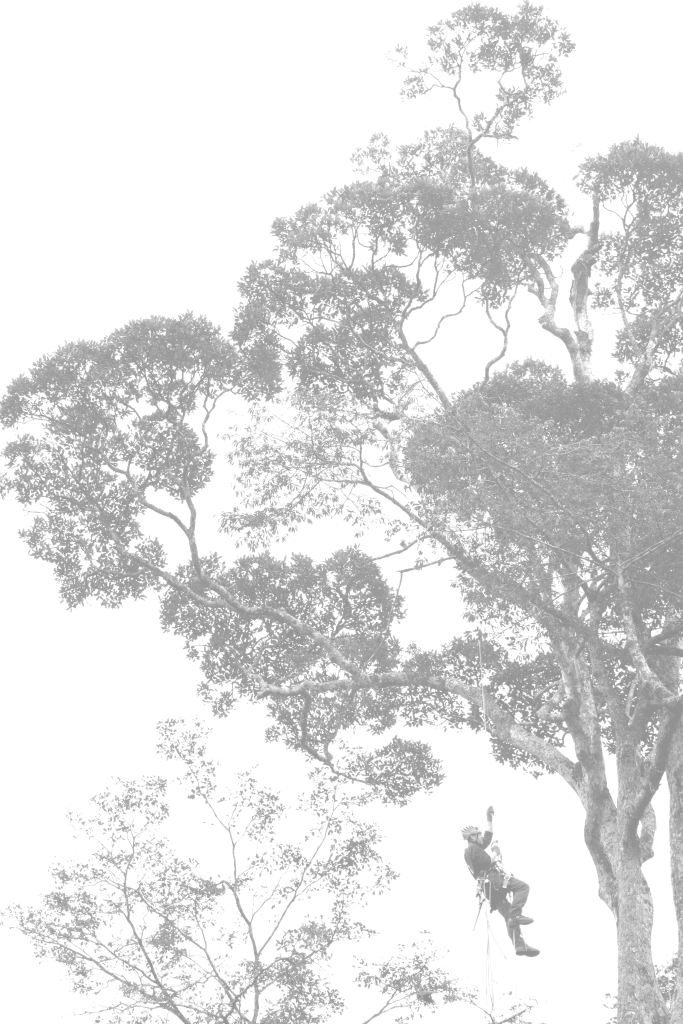
\includegraphics[width=10cm]{Filigrane}
	 \end{textblock}
	\begin{textblock}{140}[0, 1](50, 262)
		\normalfont	Version: \thedate
	\end{textblock}
	\newpage
	~\\ % Print a character or the page will not exist
	\begin{textblock}{140}(40, 40)
		#1
	\end{textblock}
	\begin{textblock}{140}[0,1](40, 270)
		\centering
    \includegraphics[width=5cm]{Logo-Lab}\\ \bigskip
		UMR \'Ecologie des forêts de Guyane\\
		\url{http://www.ecofog.gf}\\[3\baselineskip]
		Les opinions émises par les auteurs sont personnelles et n'engagent ni l'UMR EcoFoG ni ses tutelles.

    \tiny{Photographie en couverture: Hadrien Lalagüe}
	\end{textblock}
	\newpage
}


% End of preamble
%%%%%%%%%%%%%%%%%%%%%%%%%%%%%%%%%%%%%%%%%%%%%%%%%%%%%%%%%%


\begin{document}
\frontmatter

% Title page
%%%%%%%%%%%%%%%%%%%%%%%%%%%%%%%%%%%%%%%%%%%%%%%%%%%%%%%%%%

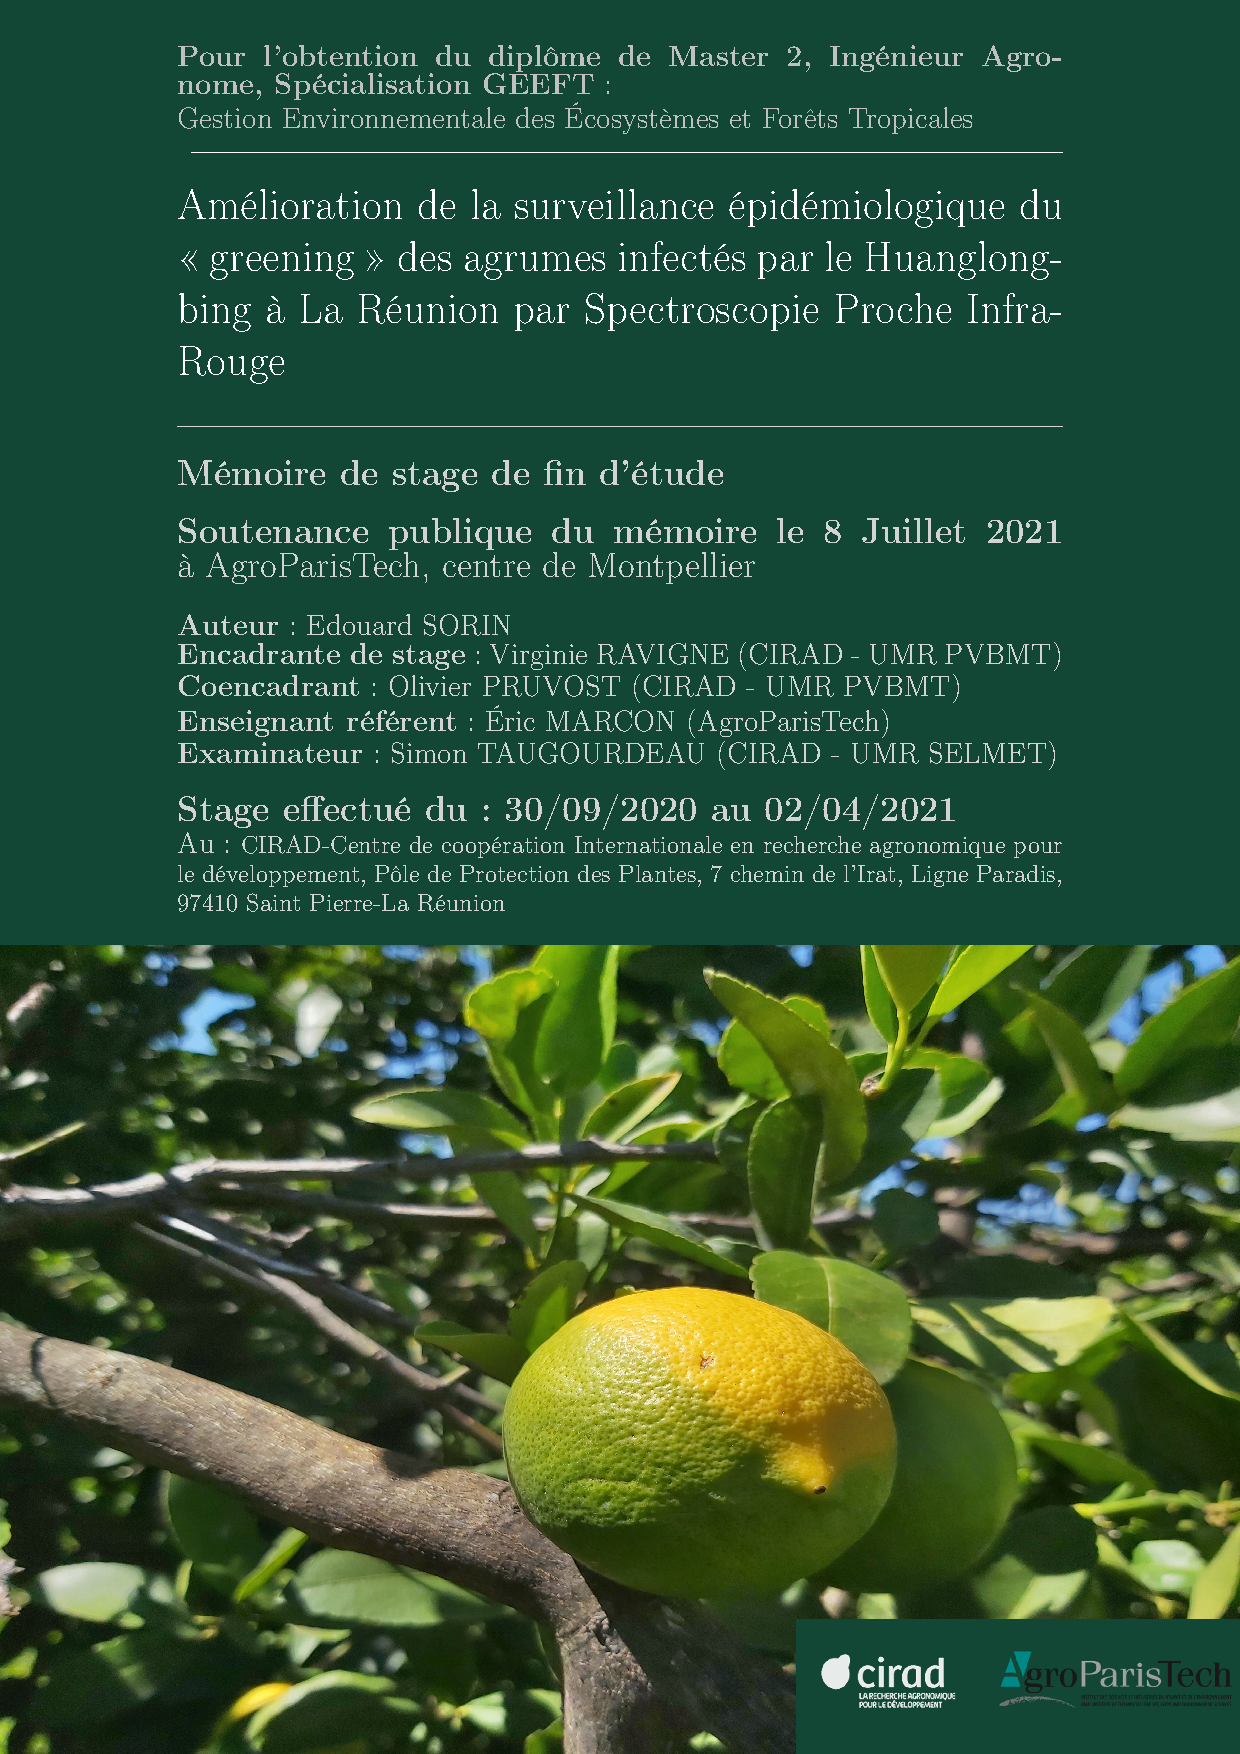
\includepdf[pages=1]{images/cover.pdf}
\cleardoublepage


% Resume/Abstract
%%%%%%%%%%%%%%%%%%%%%%%%%%%%%%%%%%%%%%%%%%%%%%%%%%%%%%%%%

\begin{description}

\selectlanguage{french}
\item[Résumé:]
Le \textbf{Huanglongbing (HLB)} est une maladie bactérienne causant le dépérissement des agrumes. Il y a une résurgence de cette maladie sur l'île de la Réunion depuis 2012, ce qui menace les vergers d'agrumes. Les techniques de détections classiques de surveillance de la maladie par PCR sont coûteuses, longues et ne peuvent pas être réalisées à grande échelle. C'est dans ce contexte qu'intervient la technologie de l'analyse par \textbf{imagerie spectrale}. Cette technologie se base sur l'analyse de la signature spectrale qu'émet un support en réponse à une exposition lumineuse. Cette méthode est non destructive pour le support traité, en plus d'être relativement peu coûteuse par rapport à la surface couverte. S'ajoute à cela un traitement des données d'imagerie spectrales par \textbf{apprentissage supervisé} dans le but de prédire le statut des arbres vis à vis de la maladie au sein des parcelles d'agrumes. Ce travail vise donc à améliorer la surveillance et la gestion de cette maladie en créant un modèle en apprentissage supervisé basé sur l'imagerie spectrale. Ce modèle est prometteur avec une qualité de la prédiction (Accuracy) de 92.6\% pour la méthode des Moindres Carrés Partiels (PLS) sur une base d'apprentissage de 8400 spectres de réflectance.

\selectlanguage{french}
\item[Mots clés :]
Apprentissage supervisé, Epidémiologie, Forêts Aléatoires (RF), HLB = Huanglongbing, Machine à Vecteurs de Support (SVM), Régression par les Moindres Carrés Partiels (PLS), Spectroscopie, Télédétection.
~\\
\vfill
\newpage
\selectlanguage{english}
\item[Abstract:]
\textbf{Huanglongbing (HLB)} is a bacterial disease causing dieback of citrus trees. There has been a resurgence of this disease on Reunion Island since 2012, which threatens citrus orchards. The conventional detection techniques for disease surveillance by PCR are expensive, time consuming and cannot be carried out on a large scale. This is where the technology of \textbf{spectral imaging} analysis comes in. This technology is based on the analysis of the spectral signature that a medium emits in response to light exposure. This method is non-destructive for the treated substrate, in addition to being relatively inexpensive compared to the surface covered. In addition, there is processing of spectral imaging data by \textbf{machine learning} in order to predict the status of trees with regard to disease within citrus plots. This work therefore aims to improve the surveillance and management of this disease by creating a supervised learning model based on spectral imaging. This model is promising with a prediction quality (Accuracy) of 92.6\% for the Partial Least Squares (PLS) method on a training base of 8400 reflectance spectra.

\selectlanguage{english}
\item[Keywords:]
Epidemiology, Machin learning, HLB = Huanglongbing, Partial Least Squares regression (PLS), Random Forests (RF), Remote sensing, Spectroscopy, Support Vector Machine (SVM).

\end{description}


% Before Body
%%%%%%%%%%%%%%%%%%%%%%%%%%%%%%%%%%%%%%%%%%%%%%%%%%%%%%%%%%





% Contents
%%%%%%%%%%%%%%%%%%%%%%%%%%%%%%%%%%%%%%%%%%%%%%%%%%%%%%%%%%

\LargeMargins
{
\hypersetup{linkcolor=}
\setcounter{tocdepth}{3}
\tableofcontents
}


% Body
%%%%%%%%%%%%%%%%%%%%%%%%%%%%%%%%%%%%%%%%%%%%%%%%%%%%%%%%%%

\LargeMargins
\hypertarget{remerciements}{%
\chapter*{Remerciements}\label{remerciements}}
\addcontentsline{toc}{chapter}{Remerciements}

Je tiens à remercier toutes les personnes qui ont contribué au bon déroulement de ce stage :

\begin{itemize}
\item
  Virginie RAVIGNE, mon encadrante de stage pour son encadrement, sa gentillesse , ses conseils et l'autonomie qu'elle m'a laissée au cours de ce stage afin que je développe mes propres axes de recherche sur cette thématique ;
\item
  Frédéric CHIROLEU, chercheur en biostatistiques, co-auteur de ce rapport, et Thuy-Trang CAO, pour leur grande aide à la réalisation des scripts R et toutes les choses apprises lors de ces rendez-vous ;
\item
  Olivier PRUVOST, pour son aide lors des analyse qPCR et son encadrement au laboratoire ;
\item
  Karine BOYER, pour m'avoir conseillé et formé aux techniques de laboratoire ;
\item
  Ismaël HOUILLON, doctorant, pour ses conseils et ses jeux de mots douteux ;
\item
  Elisa PAYET, technicienne à la FDGDON, pour avoir pris le temps de nous communiquer leurs résultats des détections du HLB et les numéros des agriculteurs ;
\item
  Raphaël SOLESSE, ainsi que Emmanuel TILLARD, pour leurs conseils, sur le pilotage de drones et la formation à l'utilisation des instruments de mesure de spectrométrie ;
\item
  Louis-Axel EDOUARD RAMBAUT, pour son aide sur les scripts R et ses discussions pertinentes ;
\item
  Claire MELOT, stagiaire au CIRAD, pour sa bonne humeur et son aide aux analyses de laboratoire tardives ;
\item
  Le CIRAD, l'équipe du 3P de Saint-Pierre et en particulier les agents de l'UMR PVBMT (Unité Mixte de
  Recherche Peuplements Végétaux et Bioagresseurs en Milieux Tropicaux) ;
\item
  Les stagiaires des Kazz pour leur amitié, les mangues et toutes les choses partagées ensemble qui ont rendu ce stage inoubliable !
\end{itemize}

\scriptsize

\normalsize

\mainmatter

\hypertarget{introduction}{%
\chapter{Introduction}\label{introduction}}

\vspace*{4cm}

\hypertarget{contexte-guxe9nuxe9ral}{%
\section{Contexte général}\label{contexte-guxe9nuxe9ral}}

La culture d'agrumes est la principale culture fruitière au monde \autocite{comte_apport_2013}. Cette culture fait face à une crise sans précédent à l'échelle mondiale due au Huanglongbing, couramment appelée HLB ou « greening », une maladie bactérienne qui est la plus dévastatrice des maladies des agrumes \autocite{moriya_detecting_2019}. Le HLB se propage rapidement et a un impact dévastateur sur la production d'agrumes dans les principales régions productrices d'agrumes du monde telles que la Chine, le Brésil, l'Inde et les Etats-Unis \autocite{deng_detection_2020}. Cette maladie a été identifiée pour la première fois en Chine il y a un siècle et depuis, 51 des 140 principaux pays producteurs d'agrumes ont été infectés par la maladie \autocite{moriya_detecting_2019}. Cependant, d'importantes régions productrices d'agrumes comme la région méditerranéenne et l'Australie sont pour le moment épargnées par cette maladie \autocite{gutierrez_prospective_2013}. Par ailleurs, \emph{Diaphorina citri}, un des insects vecteur de la maladie a été trouvé en Espagne et pose une menace immédiate de propagation du HLB dans la région méditerranéenne. En Guadeloupe le HLB a décimé la quasi-totalité des vergers et fait chuter la production agrumicole de 70\% au début de l'année 2020 \autocite{morillon_huanglongbing_2020}. Le HLB est donc devenu un problème d'échelle mondial dont la surveillance est devenue primordiale afin de limiter ses futures propagations \autocite{wang_citrus_2019}.
\vfill
\newpage
L'un des problèmes concernant la surveillance et la lutte contre cette maladie est que les différents travaux de recherche apportant des éléments concernant la lutte contre cette maladie ont été menés sur des paysages homogènes de grandes surfaces de vergers en Californie, en Floride ou au Brésil \autocite{narouei-khandan_global_2016}.
Ces travaux sont donc difficilement applicables à des paysages très hétérogènes comme à la Réunion \autocite{gottwald_current_2010}.
En effet, l'île de la Réunion est un territoire de 2 512 km² qui possède un fort gradient altitudinal, de 0 à 3070m d'altitude. S'ajoutent à cela les fortes différences d'hygrométrie entre la côte au vent à l'est et la côte sous le vent à l'ouest \autocite{guilloteau_utilisation_2018}. L'hétérogénéité éco-climatique étant importante sur ce territoire, la diversité des paysages est donc un aspect fondamental pour la surveillance de cette maladie.

Depuis 2012, le département de la Réunion avec son agriculture traditionnelle en agrumiculture est menacé par la résurgence de cette maladie (V. Ravigné, comm. pers.). A la Réunion les vergers d'agrumes sont fragmentés et ne représentent une superficie totale que de 300 ha environ \autocite{leung_production_2014}. Les vergers sont donc répartis en petites parcelles présentes sur des altitudes comprises entre 0 et 1200m \autocite{guilloteau_utilisation_2018}. Parce que la filière est peu organisée, les vergers d'agrumes sont mal répertoriés par les services de l'Etat et un travail important de l'équipe d'accueil ces dernières années a consisté à reconstruire le parcellaire agrumicole en combinant photo-interprétation d'images aériennes et vérifications sur le terrain. On dénombre, à l'issue de ce travail 682 vergers d'agrumes dont 248 infectés par le HLB \autocite{guilloteau_utilisation_2018}.
Depuis 2015, la DAAF (Direction de l'Alimentation, de l'Agriculture et de la Forêt) organise une surveillance du parcellaire agrumicole et est chargée de l'arrachage des plants contaminés. La DAAF a délégué à la FDGDON (Fédération Départementale des Groupements de Défense contre les Organismes Nuisibles) les prélèvements de matériel végétal ainsi que les tests officiels de détection de la maladie. En parallèle, l'ANSES (Agence Nationale de Sécurité Sanitaire de l'Alimentation, de l'Environnement et du Travail) en charge de la mise au point de méthodes officielles de détection est en coopération avec le CIRAD (Centre de Coopération Internationale en Recherche Agronomique pour le Développement) au travers de son UMR PVBMT (Unité Mixte de Recherche Peuplements Végétaux et Bio agresseurs en Milieu Tropical) pour l'amélioration de la détection et de la surveillance de la maladie.

\vfill
\newpage

\hypertarget{etat-des-connaissances-sur-la-maladie}{%
\section{Etat des connaissances sur la maladie}\label{etat-des-connaissances-sur-la-maladie}}

Le HLB est une maladie causée par la bactérie \emph{Candidatus} Liberibacter associée à trois sous-espèces (americanus, africanus et asiaticus) \autocite{wang_citrus_2019}. C'est la sous-espèce \emph{Candidatus} Liberibacter asiaticus que l'on retrouve sur l'île de la Réunion \autocite{aubert_greening_1989}. Cette bactérie de type Gram- (non cultivable) se développe dans les tissus riches en glucides du phloème. Cela va entraîner des nécroses dans le phloème et obstruer les vaisseaux, affaiblissant, à terme, l'arbre et entraînant sa mort \autocite{bove_huanglongbing_2006}. Le HLB est spécifique des agrumes et essentiellement transmis par les psylles qui sont des insectes de l'ordre des hémiptères. Deux espèces de psylles sont connues pour véhiculer la bactérie responsable de la maladie : \emph{Diaphorina citri} et \emph{Trioza erytreae}. Seule la première a jusqu'ici été identifiée dans l'épidémie qui sévit actuellement à la Réunion. Ces deux espèces de psylles réalisent une partie de leurs cycles de développement sur les arbres de la famille des Rutacées dont font partie les agrumes cultivés. La bactérie est transmise d'un arbre à un autre via la salive de l'insecte en se nourrissant de la sève élaborée circulant dans le phloème \autocite{narouei-khandan_global_2016}. Ce mécanisme de transmission de la maladie peut s'étendre sur une distance de 25 à 50m autour de l'arbre infecté. Cette distance peut atteindre les 1,5 km en cas de vent, ce qui favorise grandement la dispersion de la maladie \autocite{bove_huanglongbing_2006}. Par ailleurs, en plus de transmission par les psylles, le HLB peut aussi être véhiculé par les greffes et les plantes en pépinière déjà contaminées et vendues aux agrumiculteurs, ce qui fait de la gestion des pépinières un élément clé de la lutte contre la propagation de la maladie.
Le HLB affecte tous les agrumes, mais à des degrés de sensibilités différentes. La maladie provoque un dépérissement des arbres avec des symptômes visibles ressemblant à un stress hydrique ou une carence comme le jaunissement asymétrique des feuilles et des flushs (jeunes feuilles) (figure \ref{fig:1}) \autocite{bove_huanglongbing_2006}. Ces symptômes traduisent un dépérissement de l'arbre avec des fruits petits et de forme asymétrique \autocite{gottwald_preliminary_1989}.



\scriptsize

\begin{SCfigure}

{\centering 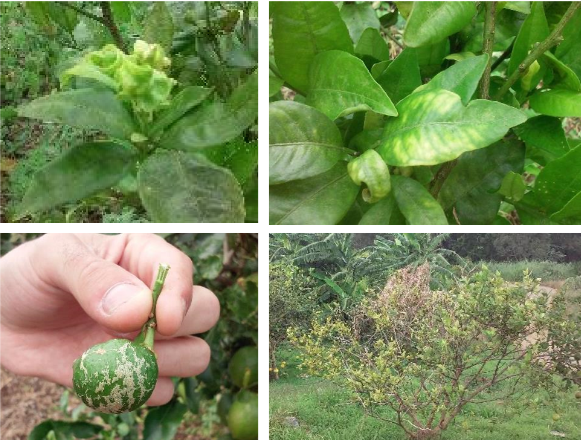
\includegraphics[width=0.8\linewidth]{Images/Figure1} 

}

\caption{Symptôme du HLB sur Flush, Feuille, Fruit et sur l'arbre \autocite{guilloteau_utilisation_2018}}\label{fig:1}
\end{SCfigure}

\normalsize

\vfill
\newpage

Cependant, les symptômes ne permettent pas l'identification de la maladie avec certitude \autocite{gottwald_preliminary_1989}. En effet, un jaunissement des feuilles peut également être causé par des carences en zinc ou en magnésium \autocite{aubert_greening_1989}. Par ailleurs, la difficulté de la détection de cette maladie réside en partie dans la période de latence qui peut durer 6 à 12 mois et durant laquelle les arbres sont parfaitement asymptomatiques tout en transmettant la maladie \autocite{bove_huanglongbing_2006}. Il a été montré que dans un verger avec 30\% d'arbres présentant des symptômes, 50\% des arbres sont déjà infectés \autocite{bove_huanglongbing_2006}. De plus, il est pour le moment difficile pour les biologistes de bien comprendre le HLB. Les défis actuels résident principalement dans le fait que \emph{Candidatus} Liberibacter ne peut être cultivée par aucune méthode \emph{in vitro} en laboratoire. Par conséquent, les analyses moléculaires et génétiques traditionnelles ont une portée limitée pour l'étude de cette bactérie \autocite{wang_citrus_2019}.

\vfill
\newpage

\hypertarget{la-ruxe9surgence-du-hlb-uxe0-la-ruxe9union}{%
\section{La résurgence du HLB à la Réunion}\label{la-ruxe9surgence-du-hlb-uxe0-la-ruxe9union}}

Le HLB avait fait l'objet d'une importante campagne d'arrachage dans les années 1970-1980 en parallèle d'une lutte chimique basée sur des produits aujourd'hui interdits (notamment des antibiotiques). Ces méthodes accompagnées d'une lutte biologique et d'un replantage de plants sains ont permis d'éradiquer cette première épidémie, une réussite unique au monde \autocite{gottwald_preliminary_1989}. La lutte biologique a reposé sur l'introduction de parasitoïdes des psylles permettant un contrôle des populations de psylles vecteurs de la maladie, encore actifs aujourd'hui \autocite{aubert_case_1996}. Cependant, depuis 2012, de nouveaux cas de HLB ont été observés sur l'île. Les parasitoïdes étant toujours présents, aucune pullulation de psylles n'est relevée et c'est uniquement \emph{D. citri} qui est observé \autocite{guilloteau_utilisation_2018}. Si la cause de cette résurgence ne vient pas d'une pullulation de la population de psylles, elle pourrait provenir de vergers comportant des arbres malades non arrachés lors de la première épidémie, d'un relâchement des pratiques en pépinière ou d'une introduction accidentelle \autocite{guilloteau_utilisation_2018}.

En l'absence de traitement, l'arrachage précoce des arbres malades est pour l'instant le moyen le plus efficace de lutte contre cette épidémie. Cependant, cette méthode est coûteuse en moyens humains et financiers. L'arrachage lui-même est une procédure complexe et après replantation un verger ne rentre en production qu'au bout de plusieurs années (4 à 6 ans), ce qui constitue un manque à gagner important. Les aides financières sont très limitées et ne concernent actuellement que la replantation. Dès lors, l'acceptabilité de la lutte par arrachage est mauvaise. De plus, la technique officielle de détection et surveillance de la maladie par PCR est coûteuse, de réalisation laborieuse et peut donc difficilement être déployée à grande échelle. De ce fait, la stratégie de surveillance officielle actuelle qui est d'analyser 60 arbres à l'hectare ne permet pas aux agriculteurs de savoir précisément le statut de chaque arbre dans leur parcelle, ce qui diminue encore l'acceptabilité des mesures d'arrachage. Permettre aux agriculteurs de disposer d'une information sur le statut de chaque arbre dans leur parcelle est un levier essentiel pour les amener à prendre les décisions difficiles que l'épidémie leur impose.\\
D'autres moyens de surveillance doivent donc être mis en place. C'est dans ce contexte qu'intervient la technologie de l'analyse par imagerie spectrale. Cette technologie se base sur l'analyse de la signature spectrale mesurée en réflectance qu'émet un support en réponse à une exposition lumineuse \autocite{sankaran_huanglongbing_2013}. Cette technologie présente plusieurs avantages prometteurs pour la détection du HLB. En effet, cette méthode est non destructive pour le support traité, est relativement peu coûteuse par rapport à la surface couverte et l'efficacité de l'analyse est importante à condition de trouver un calibrage optimal pour détecter la maladie \autocite{sankaran_visible-near_2011}. Réalisée par des spectromètres à main, cette technique pourrait en principe permettre d'augmenter significativement les cadences de détection de la maladie et ainsi fournir à bas coût une information complète aux agriculteurs touchés quant à l'état de leur verger. Des tentatives de détecter le HLB par ses signatures spectrales existent dans la littérature scientifique \autocite{sankaran_visible-near_2011} et elles sont encourageantes mais le contexte réunionnais est particulier.
Les nombreuses variétés locales n'ont jamais été testées dans la littérature, même les plus importantes (tangor, mandarine zanzibar, orange navel, citron quatre saisons\ldots) car les recherches sont principalement concentrées sur les citronniers, les orangers et les mandariniers \autocite{sankaran_visible-near_2011} \autocite{deng_detection_2020}. Comme les agrumes sont souvent une culture secondaire dans des exploitations centrées sur autre chose (canne, maraîchage), les arbres sont souvent cultivés de façon non optimale, peu technique et donc peuvent souffrir de carences nutritives et de déficit hydrique. Ces éléments font que les signatures spectrales du HLB pourraient être moins claires à la Réunion que dans les conditions testées ailleurs. Au cours de ce stage, je répondrai ainsi à la question suivante : \textbf{Peut-on développer une méthode de la télédétection par imagerie spectrale fiable pour améliorer la surveillance épidémiologique du Huanglongbing (HLB) à La Réunion ?}

L'objectif global va donc être de prédire le statut positif ou négatif au HLB des arbres directement avec des outils de télédétection.

Pour résoudre cette problématique, je traiterai les objectifs spécifiques suivants :

\begin{enumerate}
\def\labelenumi{\arabic{enumi})}
\tightlist
\item
  Les différentes parcelles et variétés analysées ont elles une influence sur les résultats visant à prédire l'état sanitaire des arbres ?
\item
  Quelles longueurs d'onde sont les plus discriminantes pour la recherche de la maladie par télédétection ?
\item
  Peut-on connaître l'état sanitaire d'un arbre via une analyse par télédétection ? Sous quel degré de précision ?
\end{enumerate}

\hypertarget{matuxe9riel-et-muxe9thodes}{%
\chapter{Matériel et Méthodes}\label{matuxe9riel-et-muxe9thodes}}

\hypertarget{identification-de-la-maladie}{%
\section{Identification de la maladie}\label{identification-de-la-maladie}}

Pour l'analyse en télédétection, les feuilles analysées doivent avoir un statut connu vis-à-vis de la maladie. Afin de connaître le statut et mettre en évidence cette maladie difficilement détectable dans les vergers, la méthode de détection par PCR (Polymerase Chain Reaction) est pour l'instant la plus utilisée pour surveiller l'évolution de la maladie. Cette méthode permet de détecter l'ADN de la bactérie à partir d'échantillons de feuilles \autocite{gottwald_current_2010}. L'inconvénient de cette méthode est qu'elle ne permet pas le traitement d'un volume important d'échantillons et ne donne pas une réponse immédiate sur le prélèvement effectué sur le terrain. La PCR est une technique reconnue de multiplication de l'ADN d'un échantillon. Le but est de dupliquer les échantillons d'ADN prélevés à chaque cycle de réaction via l'ADN polymérase. Ainsi, avec un seul brin d'ADN de départ, des millions de répliques sont produites à chaque cycle de réplication. La qPCR repose sur le même principe avec des améliorations de la technique de départ. Le principe est toujours de multiplier l'ADN de l'échantillon, mais avec cette fois une quantification du nombre de cycles PCR nécessaires à la détection de la maladie. Le nombre de cycles de réplication ou Cycle Threshold (Ct) correspond au nombre de cycles PCR à partir duquel le produit de la PCR est détectable. Ainsi, plus le Ct est faible plus il y a d'ADN présent initialement et inversement. Les échantillons sains et malades peuvent donc être distingués selon leur valeur de Ct selon un seuil fixé.
La méthode officielle actuelle basée sur la PCR classique est actuellement en cours de remplacement par une méthode basée sur la qPCR et qui utilisera le seuil de 36 cycles de détection maximum pour identifier un échantillon comme étant porteur de la maladie. C'est ce seuil de 36 cycles ou Ct36 qui sera utilisé dans cette étude pour statuer de l'état malade ou sain des arbres.

\hypertarget{choix-des-arbres}{%
\section{Choix des arbres}\label{choix-des-arbres}}

Le choix des parcelles échantillonnées a été conditionné par la recherche d'un équilibre entre les arbres malades et sains sur chaque parcelle basée sur les données compilées par le CIRAD issu de la FDGDON et de la DAAF. Le défi étant que les statuts des arbres ne sont pas connus à l'avance et il peut être compliqué de faire un design équilibré en amont de la récolte de données. L'objectif a donc été dans un premier temps de trouver les agriculteurs qui possèdent les trois variétés d'agrumes sur lesquelles se base cette étude, à savoir les citrons (\emph{Citrus limon}), les mandarines zanzibar (\emph{Citrus reticulata}) et les tangors (\emph{Citrus reticulata x sinensis}). Dans un deuxième temps, pour chacun de ces agriculteurs il a fallu identifier précisément le statut des arbres.

Concernant les caractéristiques altitudinales et pluviométriques des parcelles, celle de Mr Hoarau et Mr Pothin échantillonnées à Petite-Ile sont comprises dans une échelle de pluviométrie identique la parcelle de Mr Gonthier échantillonnée dans les hauts du Tampon à savoir entre 1430 et 1680 mm de pluie par an \autocite{equipe_artists_-_ur_aida_meteor_2021}. Leurs altitudes respectives sont cependant très différentes avec une différence de 1000 m et plus entre la parcelle du Tampon et les autres (figure \ref{fig:2}). La parcelle de Mr Barret située au niveau de la mer est la parcelle qui reçoit le moins de précipitation avec seulement 930 à 960 mm de pluie par an \autocite{equipe_artists_-_ur_aida_meteor_2021}.

\scriptsize

\begin{SCfigure}

{\centering \includegraphics[width=0.8\linewidth]{Images/Figure2} 

}

\caption{Carte présentant les parcelles échantillonnées, leurs dates de prélèvement ainsi que la pluviométrie et les altitudes}\label{fig:2}
\end{SCfigure}

\normalsize

L'échantillonnage a commencé dans la commune de Petite-Ile, qui est la plus grosse zone de production d'agrumes de l'île (environ 25\% de la surface en agrumes) \autocite{guilloteau_utilisation_2018}. Cette zone est aussi très touchée par le HLB (près de 2 parcelles sur trois) avec par conséquent, des prospections importantes de la part de la DAAF et de la FDGDON qui fournissent des données précieuses pour l'échantillonnage. Les parcelles de Mr Hoarau et Mr Pothin échantillonnées à Petite-Ile possèdent les trois variétés recherchées mais ont une répartition différente entre les arbres malades et sains.
\vfill
\newpage
Dans la parcelle de Mr Hoarau l'échantillonnage s'est basé sur une première cartographie des statuts HLB des arbres réalisée dans le cadre d`une expérimentation de la FGDGON pour le développement d'une autre méthode moléculaire. 42 arbres ont ainsi été sélectionnés dont 19 arbres se sont révélés sains et 23 arbres se sont révélés infectés par le HLB (figure \ref{fig:3}).

\scriptsize

\begin{SCfigure}

{\centering 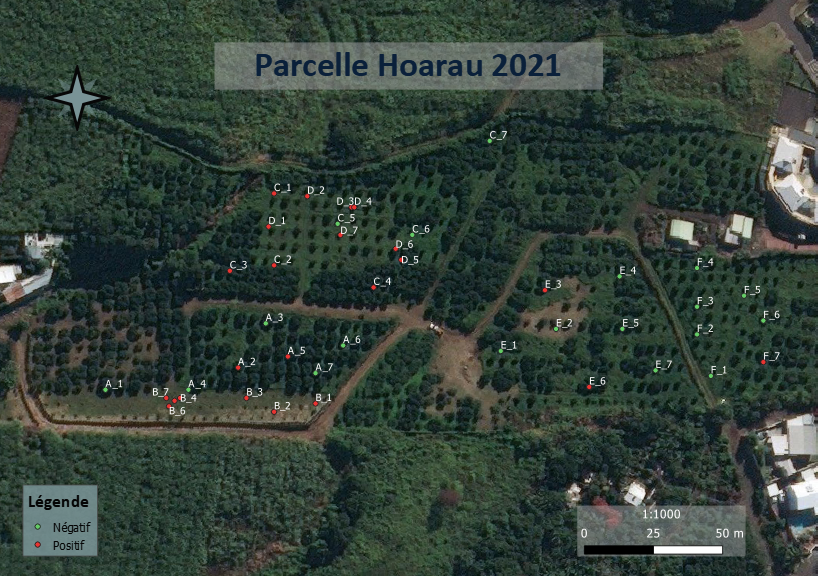
\includegraphics[width=0.8\linewidth]{Images/Figure3} 

}

\caption{Échantillonnage réalisé dans la parcelle de Mr Hoarau en 2021}\label{fig:3}
\end{SCfigure}

\normalsize

A l'inverse dans la parcelle de Mr Pothin, l'échantillonnage des arbres en se basait sur les dires d'expert de l'agriculteur et trouvé trois arbres sains pour 39 arbres infectés par le HLB (figure \ref{fig:4}).

\scriptsize

\begin{SCfigure}

{\centering 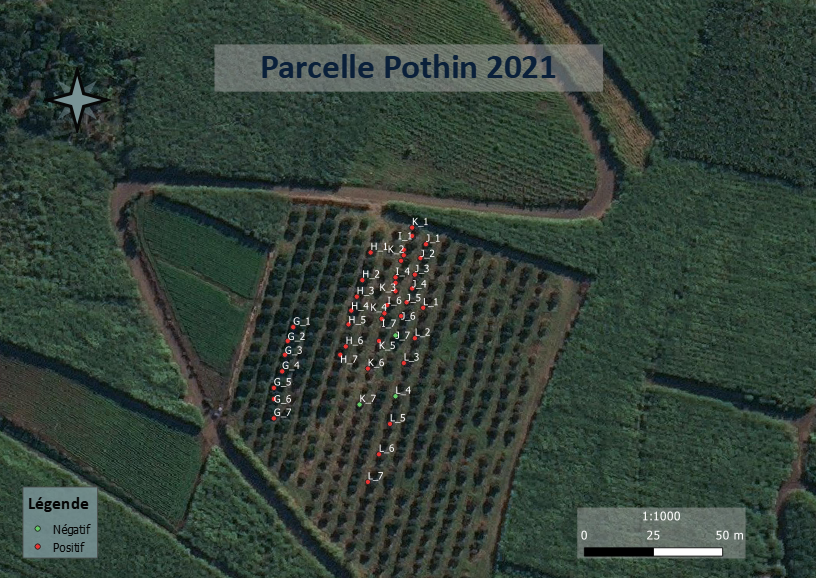
\includegraphics[width=0.8\linewidth]{Images/Figure4} 

}

\caption{Échantillonnage réalisé dans la parcelle de Mr Pothin en 2021}\label{fig:4}
\end{SCfigure}

\normalsize

La parcelle de Mr Barret située à St Pierre et constituée uniquement de citronniers a été échantillonnée de manière exhaustive. Cette parcelle fut la plus analysée en laboratoire. Les 156 arbres de la parcelle ont d'abord été regroupés par pools de 5 puis certains arbres ont été analysés individuellement selon leurs statuts. Au final 10 citronniers sains et quatre infectés par le HLB ont été trouvés (figure \ref{fig:5}).

\scriptsize

\begin{SCfigure}

{\centering 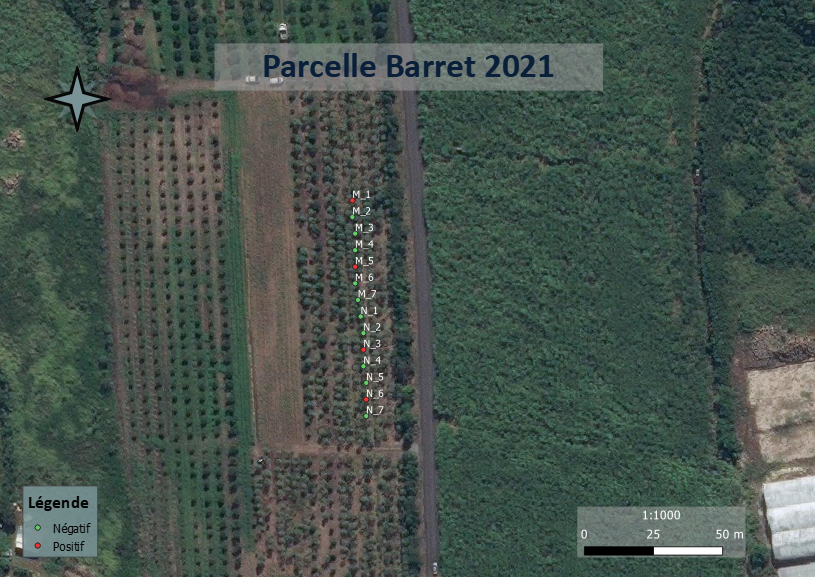
\includegraphics[width=0.8\linewidth]{Images/Figure5} 

}

\caption{Échantillonnage réalisés dans la parcelle de Mr Barret en 2021}\label{fig:5}
\end{SCfigure}

\normalsize
\vfill
\newpage
A l'issue de cet échantillonnage, un grand nombre d'arbres infectés chez Mr Pothin et Barret ont été trouvés, il y avait donc un déficit d'arbres sains. La parcelle de Mr Gonthier située au Tampon a donc été trouvée pour pallier à ce déficit. Cette parcelle compte une répartition égale entre les trois variétés et dont les arbres ont été testés négatifs aux HLB en novembre 2020 par la FDGDON. Pour chaque variété 14 arbres ont été échantillonnés (figure \ref{fig:6}) afin de rééquilibrer l'ensemble du jeu de données. Cet échantillonnage n'est pas idéal, dans la mesure où les facteurs agriculteur et variété ne sont pas croisés, et une attention particulière sur ce point devra être portée dans l'interprétation des résultats.

\scriptsize

\begin{SCfigure}

{\centering 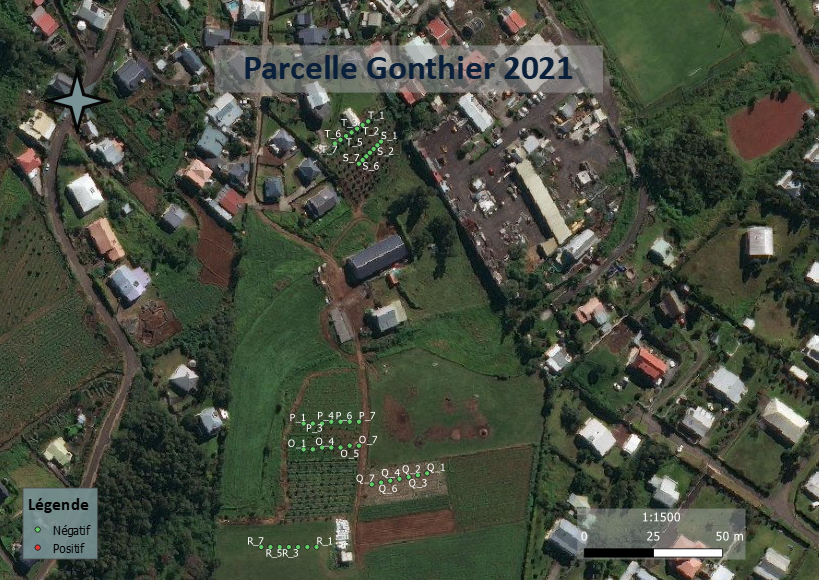
\includegraphics[width=0.8\linewidth]{Images/Figure6} 

}

\caption{Échantillonnage réalisés dans la parcelle de Mr Gonthier en 2021}\label{fig:6}
\end{SCfigure}

\normalsize

Au final, au cours de cette étude 140 arbres ont été échantillonnés et numérotés de A1 à T7. Le choix de faire des groupes de sept arbres auxquels une lettre est affiliée vient du fait que les plaques nécessaires à l'analyse ont 28 emplacements pouvant ainsi analyser quatre groupes de sept arbres.

\vfill
\newpage

\hypertarget{spectroscopie-uxe0-main}{%
\section{Spectroscopie à main}\label{spectroscopie-uxe0-main}}

L'objectif de l'utilisation de la spectroscopie est la discrimination des arbres sains et malades de façon rapide et clairement identifiable en passant l'outil de détection sur la parcelle. La détection de la maladie sur les plantes repose sur la capacité des feuilles à absorber, réfléchir ou transmettre la lumière dans différentes longueurs d'onde mesurées en nanomètre (nm). Ces caractéristiques sont liées à la composition biochimique des feuilles. Les variations de mesure de spectre peuvent donc être expliquées dans les différents domaines du spectre par la teneur en pigment des feuilles dans le visible (400-750nm), par la structure cellulaire avec l'essentiel des vaisseaux dont le phloème dans le proche infrarouge (750-1250 nm) et par la teneur en eau dans le ``Short-wave infrared'' ou SWIR (1250-2500 nm) comme indiqué sur la (figure \ref{fig:7}) \autocite{comar_etude_2013}. Les bandes spectrales du visible (bleu, vert, rouge, ``red-edge'') sont les plus utilisées dans la détection de maladie des feuilles \autocite{mishra_spectral_2007}. La qualité des résultats dépend de la résolution du capteur utilisé.
Dans le visible (400-750nm), la coloration des feuilles est due à la teneur en chlorophylles, caroténoïdes et anthocyanes. Les chlorophylles (de type a et b) captent la lumière dans des longueurs d'ondes correspondant au bleu et au rouge.
Les caroténoïdes captent la lumière exclusivement dans le bleu et les anthocyanes la captent exclusivement dans le vert. Vers la fin du domaine visible (700nm) il n'y a plus de captage de lumière aussi important et la lumière est quasiment entièrement réfléchie dans cette zone appelée ``red edge''.
Ensuite, la zone du proche infrarouge (750-1250 nm) correspond principalement à la structure cellulaire interne des feuilles qui est aussi peu affectée en cas de maladie. Cette zone est utile pour la discrimination des feuilles entre feuillus et résineux qui ont des structures de tissus différentes.
Enfin, dans le SWIR (1250-2500 nm), c'est principalement la teneur en eau des feuilles qui est mesurée. Plus la réflectance est faible, plus la teneur en eau est grande, ce qui est utile pour caractériser un stress hydrique chez la plante \autocite{albetis_de_la_cruz_potentiel_2018}.

\scriptsize

\begin{SCfigure}

{\centering 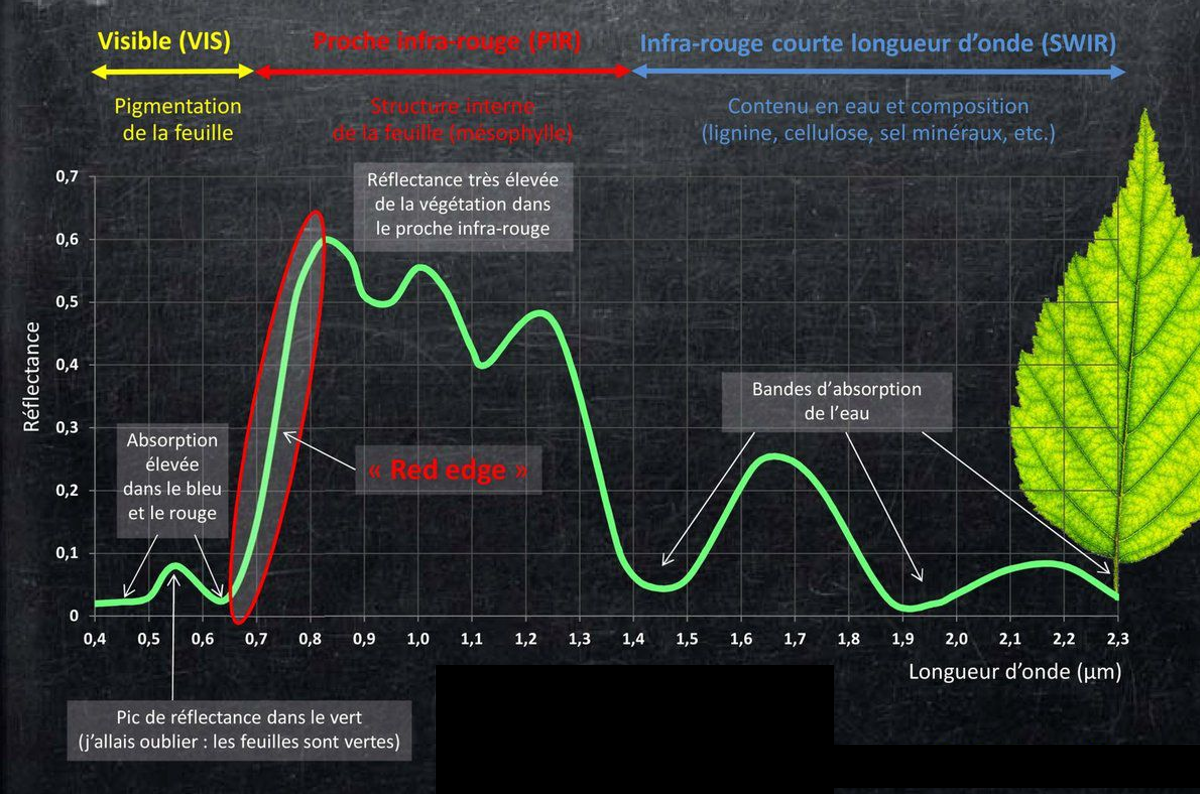
\includegraphics[width=0.8\linewidth]{Images/Figure7} 

}

\caption{Schéma de la variation de la réflectance de la végétation}\label{fig:7}
\end{SCfigure}

\normalsize

Au cours de cette étude, la détection du statut infecté en HLB des arbres va être réalisés par la méthode de la Spectroscopie Proche Infra-Rouge (SPIR) à main qui est catégorisée comme étant de la proxidétection \autocite{albetis_de_la_cruz_potentiel_2018}.
Dans le cas de la proxidétection, l'acquisition des données se fait par contact direct ou à quelques centimètres de l'objet cible à l'échelle de la feuille ou de la plante (figure \ref{fig:8}).

\scriptsize

\begin{SCfigure}

{\centering 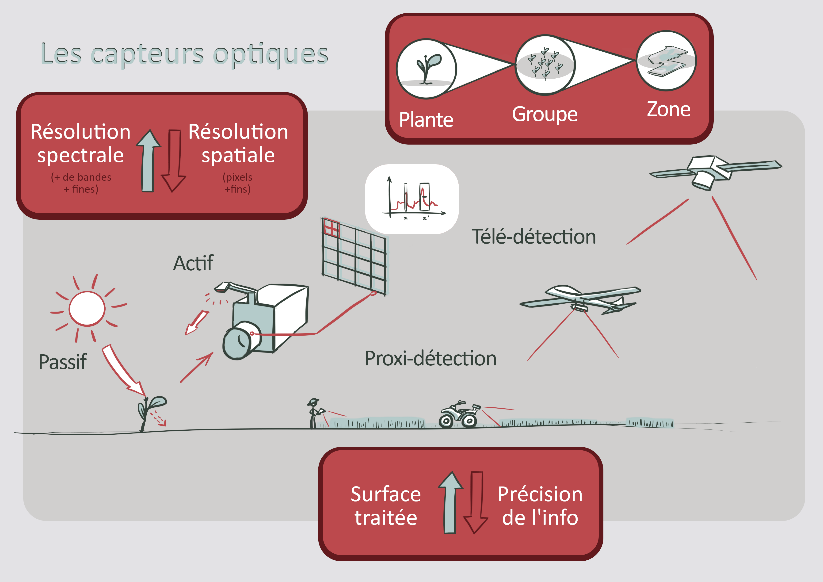
\includegraphics[width=0.8\linewidth]{Images/Figure8} 

}

\caption{Schéma d’application des capteurs optiques}\label{fig:8}
\end{SCfigure}

\normalsize

Ainsi, pour l'acquisition des données, un spectromètre de terrain (ASD fieldspec Pro) a été utilisé en laboratoire (figure \ref{fig:9}). L'appareil est utilisé afin de mesurer la réflectance, une mesure correspondant à la proportion (comprise entre 0 et 1) de lumière réfléchie par la surface d'un matériau qui est ici une feuille d'agrume \autocite{comar_etude_2013}.
Afin de mesurer cette réflectance, la feuille disposée sur un disque blanc en Spectralon® qui renvoie quasiment toute la lumière transmise. Cette lumière transmise par l'appareil traverse d'abord la feuille puis est réfléchie et retraverse la feuille avant d'atteindre le capteur. Le Spectralon® est régulièrement nettoyé au papier de verre pour conserver sa valeur de réflectance constante au cours du temps. De plus, les mesures sont réalisées à température ambiante et un blanc est effectué toutes les 15 minutes en réalisant une mesure de SPIR sur le support en Spectralon® seul. L'appareil mesure une bande de longueur d'onde allant de 350 à 2500 nm, la courbe caractérisant la réflectance en fonction des longueurs d'onde mesurées est appelée spectre de réflectance \autocite{comar_etude_2013}.
Pour chaque mesure, le spectre de réflectance correspond à une moyenne de 50 mesures de réflectance effectuées par l'appareil entre 350 et 2500 nm.

\scriptsize

\begin{SCfigure}

{\centering 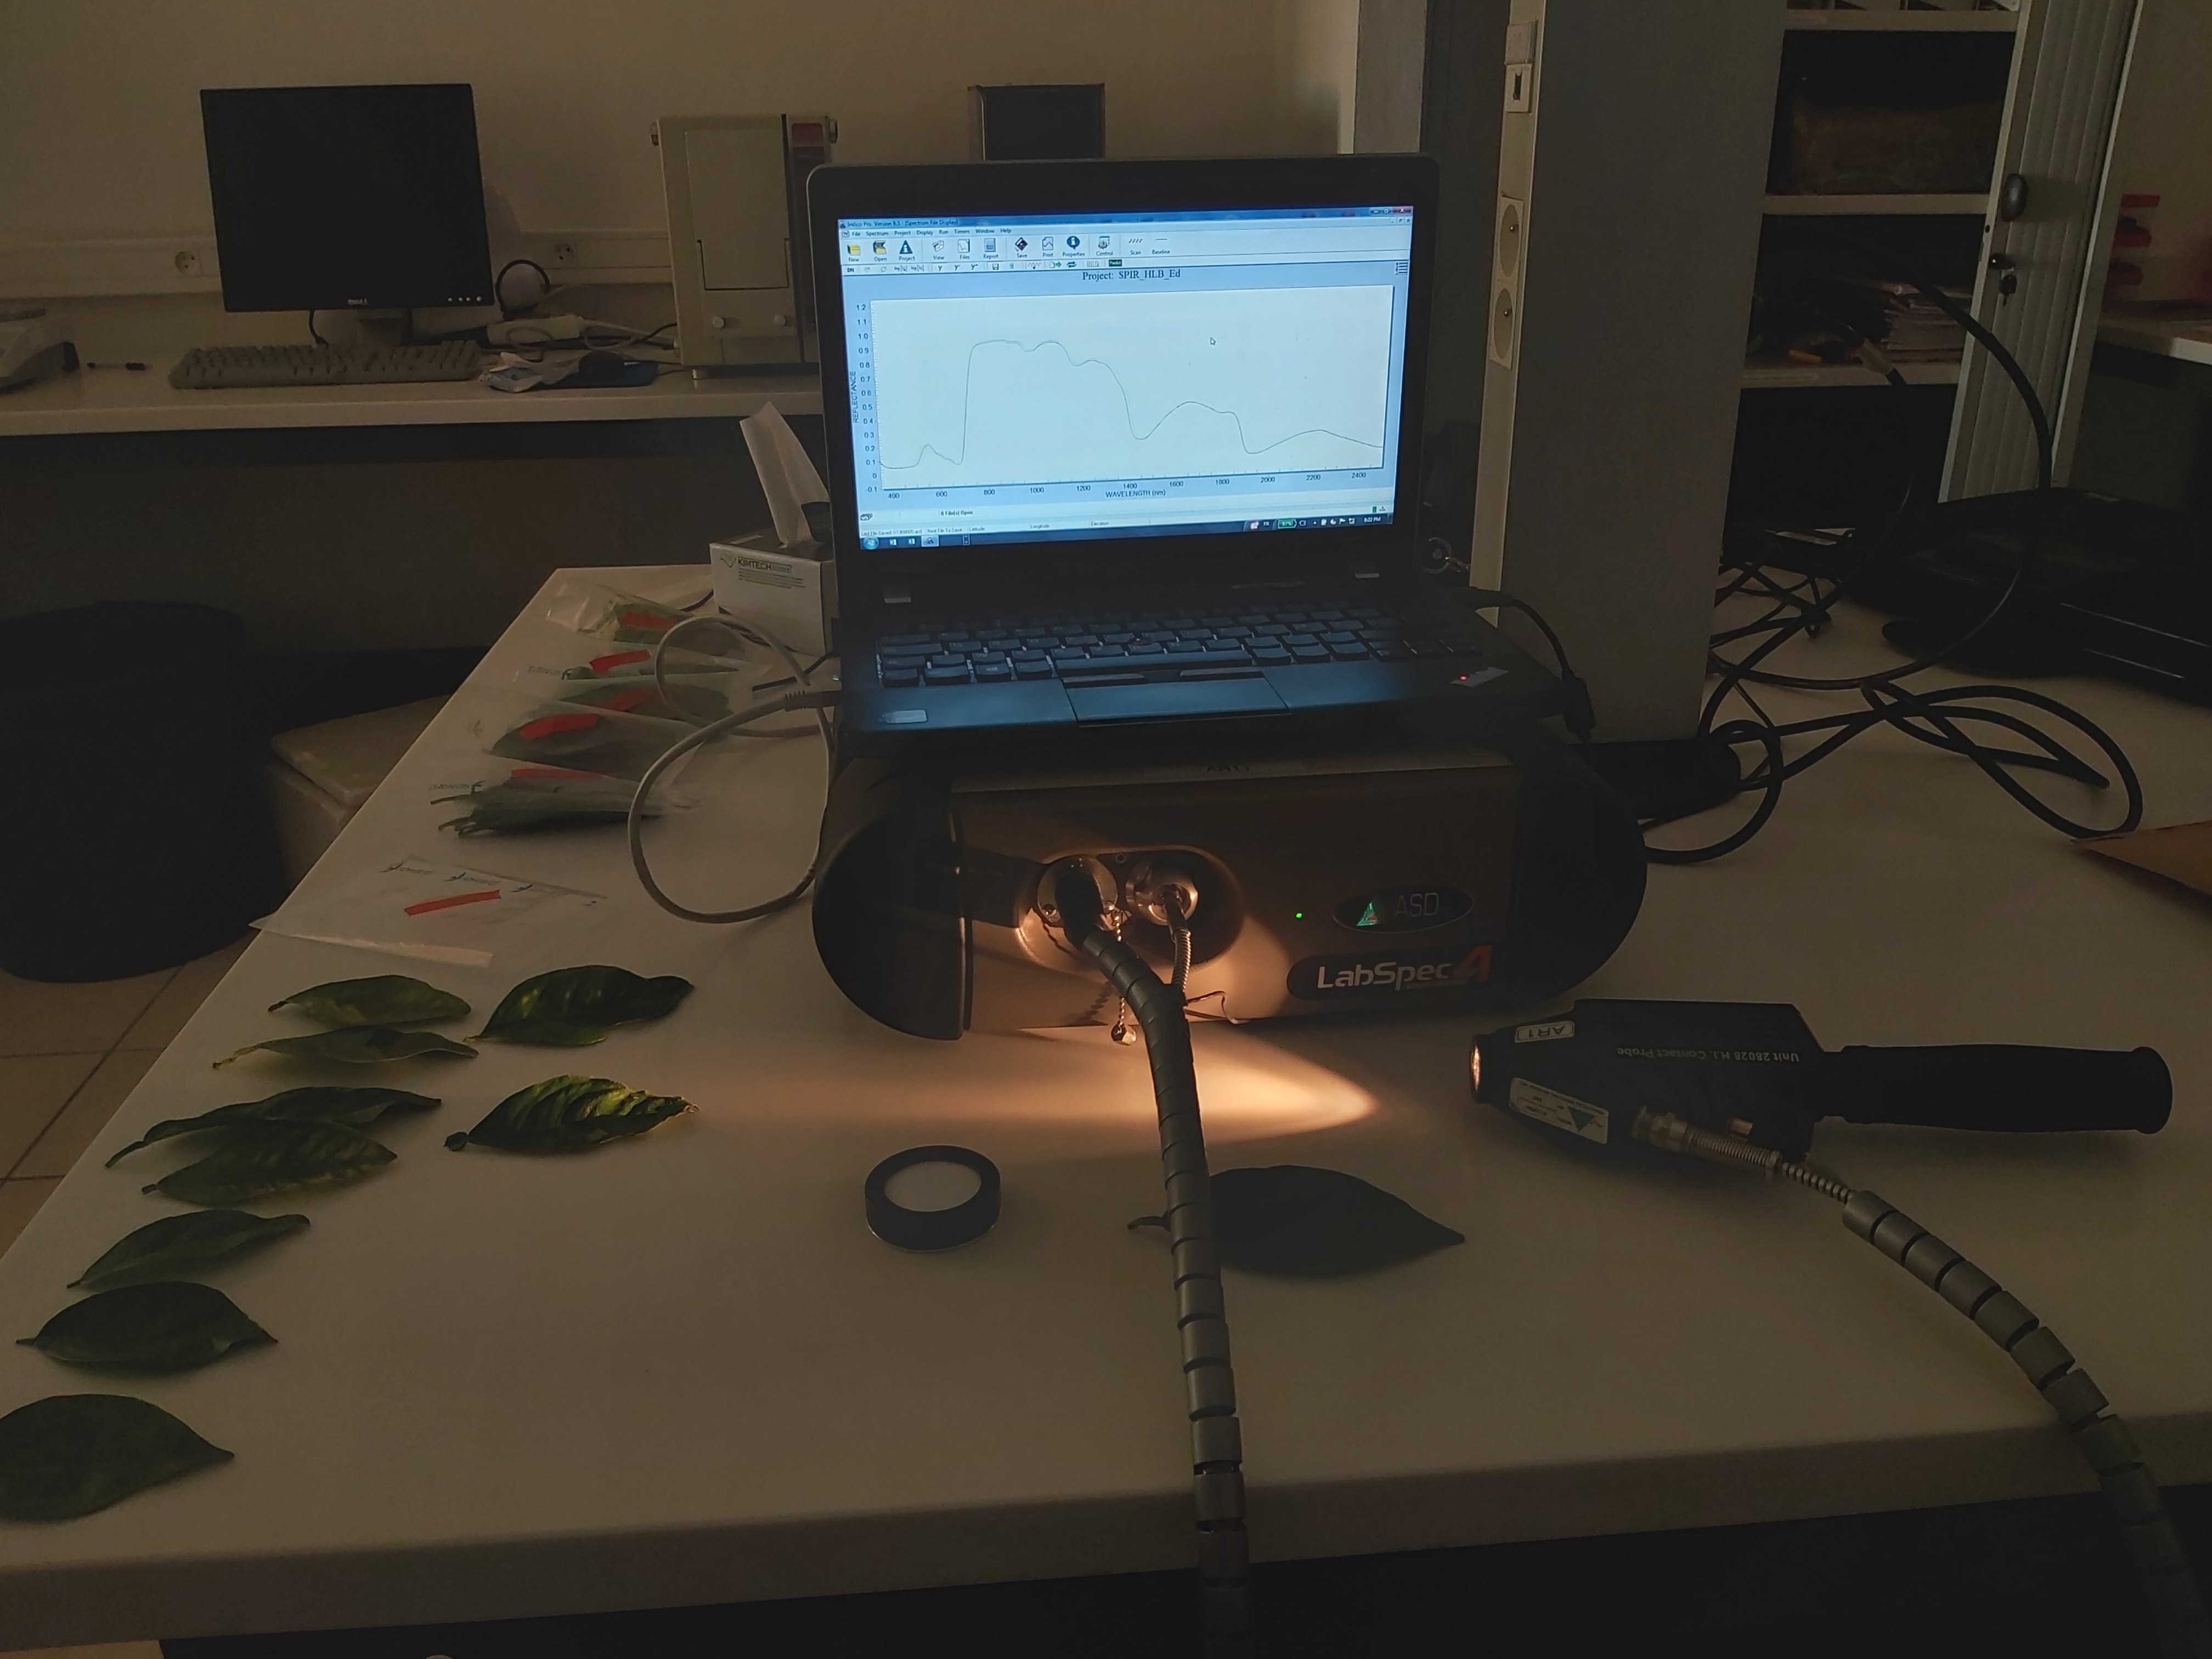
\includegraphics[width=0.8\linewidth]{Images/Figure9} 

}

\caption{Photographie d’un spectromètre proche infra-rouge à main}\label{fig:9}
\end{SCfigure}

\normalsize

Sur chaque arbre 10 feuilles sont prélevées de manière aléatoire autour de l'arbre. Le nombre de 10 feuilles à échantillonner provient d'un compromis entre le temps d'analyse de ces feuilles et de la précision des résultats recherchés. Ce compromis n'aurait pas pu être possible sans les travaux de Nathan Créquy qui avait prélevé trois lots de 10 feuilles sur 14 arbres échantillonnés et sur lesquelles des tests sur la baisse de précision ont pu être effectués avant d'aboutir au nombre idéal de feuilles à prélever \autocite{crequy_prise_2020}.Sur chacune des 10 feuilles prélevées par arbre, six mesures de réflectance sont réalisées afin d'avoir des spectres de réflectance issus des différentes zones de la feuille. Ce nombre de mesures optimal fut calculé en amont via les données issues de l'étude de Nathan Créquy qui avait 10 mesures SPIR par feuille et dont les paramètres de précision furent comparés au moyen de tests statistiques pour chaque mesure effectuée par feuille \autocite{crequy_prise_2020}.En fonction des longueurs d'onde étudiées, les capteurs utilisés sont différents et regroupés en deux catégories, les capteurs multispectraux et hyperspectraux. Les capteurs multispectraux permettent d'enregistrer des bandes spectrales qui ne sont pas contiguës et qui peuvent être ciblées, par exemple : le proche infrarouge, le bleu, le rouge et le vert. A l'inverse, les capteurs hyperspectraux enregistrent plus ou moins toutes les bandes spectrales (en fonction de la résolution de l'appareil) de façon contiguë dans un intervalle de longueur d'onde compris entre 350 et 2500 nm \autocite{bertaux_mise_2015}. Au cours de cette étude, seul le capteur hyperspectral sera utilisé sur la partie SPIR avec six mesures SPIR par feuille sur les 10 feuilles prélevées par arbres.
Le jeu de données (annexe 1) est donc composé en détail du :

\scriptsize

\normalsize
- nombre d'arbres échantillonnés

\scriptsize

\begin{verbatim}
[1] 140
\end{verbatim}

\normalsize

\begin{itemize}
\tightlist
\item
  nombre de feuilles échantillonnées et analysées en SPIR
\end{itemize}

\scriptsize

\begin{verbatim}
[1] 1400
\end{verbatim}

\normalsize

\begin{itemize}
\tightlist
\item
  nombre réel de données comprenant les 6 répétitions SPIR par feuilles échantillonnées
\end{itemize}

\scriptsize

\begin{verbatim}
[1] 8400
\end{verbatim}

\normalsize

\vfill
\newpage

\hypertarget{traitement-des-donnuxe9es-par-analyses-statistiques-et-apprentissage-supervisuxe9}{%
\section{Traitement des données par analyses statistiques et apprentissage supervisé}\label{traitement-des-donnuxe9es-par-analyses-statistiques-et-apprentissage-supervisuxe9}}

Tous les traitements statistiques sont réalisés sous R \autocite{R}

Les données utilisées pour les analyses sont les valeurs de réflectance issues de la SPIR à main allant de 350 à 2500 nm.

Dans un premier temps, l'objectif va être de caractériser les sources de variations des spectres de réflectance, et en particulier, l'influence des parcelles et des variétés sur ces derniers. Ainsi pour chaque longueur d'onde, une décomposition de la variance est mise en œuvre via une ANOVA à un facteur où la variable expliquée est la réflectance observée pour cette longueur d'onde et la variable explicative est la variété ou la parcelle. Cette analyse produit pour chaque longueur d'onde une valeur du F de Fisher correspondant au rapport entre la variance intermodalités (entre parcelles ou entre variétés) et la variance résiduelle (au sein des parcelles ou des variétés). Plus le F de Fisher est élevé, plus la variable testée (parcelle ou variété) affecte la réflectance.

Une fois démontrée l'influence ou la non-influence de ces variables de nuisance, il est possible d'envisager une prédiction sur le statut HLB des arbres à partir des spectres de réflectance. Pour ce faire, trois types de méthodes de classification par apprentissage supervisé sont mis en œuvre : les forêts aléatoires (RF pour « Random Forest» ), la machine à vecteurs de support (SVM pour « Support Vector Machine ») et la régression par les moindres carrés partiels ( PLS pour « Partial Least Square »).

Un algorithme d'apprentissage supervisé se compose à la fois de données d'entrée ``training set'' (75\% de la base d'apprentissage) et de données cibles ``test set'' (25\% de la base d'apprentissage). Les données d'entrée comprennent des spectres de réflectances associés à un statut HLB. Elles permettent à l'algorithme de « s'entrainer » à reconnaître le statut HLB des arbres à partir des spectres de réflectance. Les données cibles (test) sont composées de spectres pour lesquels le statut HLB est connu mais ne peut être utilisé par l'algorithme car ces données sont utilisées pour la vérification et pour éviter la redondance d'utilisation d'une donnée dans l'apprentissage. Elles permettent de mesurer la performance de l'algorithme. Après s'être assuré de la bonne performance de l'algorithme, on peut l'utiliser pour prédire le statut HLB d'arbres dont on ne dispose que du spectre de réflectance.

\vfill
\newpage

\hypertarget{foruxeats-aluxe9atoires-rf}{%
\section{Forêts Aléatoires (RF)}\label{foruxeats-aluxe9atoires-rf}}

Les RF est une technique utilisant un algorithme d'apprentissage supervisé couplé avec un arbre de décision \autocite{randomForest}. Un arbre de décision est une construction de choix souvent binaire qui permet de prendre une décision. Cet algorithme permet de créer une forêt d'arbres de décision qui permet d'améliorer la généralisation (sur un paramètre recherché) de l'ensemble du modèle. La RF combine la simplicité de lecture des arbres de décision ainsi que la robustesse de l'apprentissage supervisé qui améliore la précision de la prédiction \autocite{moutarde_arbres_2017}.
La première étape de la construction du RF est la création d'un jeu de données pour chaque arbre de décision (figure \ref{fig:11}). Ce jeu de données se compose des lignes des données originelles piochées aléatoirement (la même ligne pouvant être sélectionnée plusieurs fois comme la ligne 2 de l'exemple en rouge). Ce procédé augmente la variété des arbres de décision ce qui rend l'algorithme encore plus robuste \autocite{moutarde_arbres_2017}.

\scriptsize

\begin{SCfigure}

{\centering 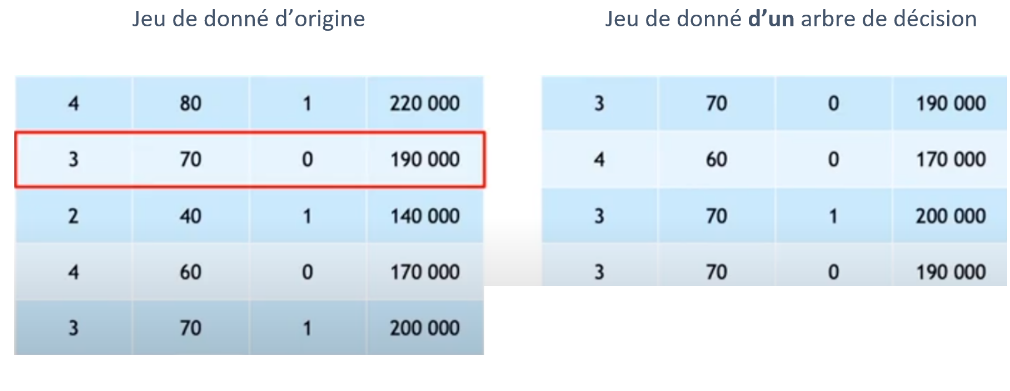
\includegraphics[width=0.8\linewidth]{Images/Figure11} 

}

\caption{Schéma 1 de construction d’un jeu de données d’un arbre de décision en RF}\label{fig:11}
\end{SCfigure}

\normalsize

\vfill
\newpage

La deuxième étape va être la création de chaque arbre de décision sur une partie différente (aléatoire et non exclusive) des données et des variables à l'intérieur de leurs jeux de données (figure \ref{fig:12}, rectangles de couleurs). L'intérêt est d'avoir des estimateurs différents dans chaque arbre de décision pour avoir un cheminement différent \autocite{moutarde_arbres_2017}.

\scriptsize

\begin{SCfigure}

{\centering 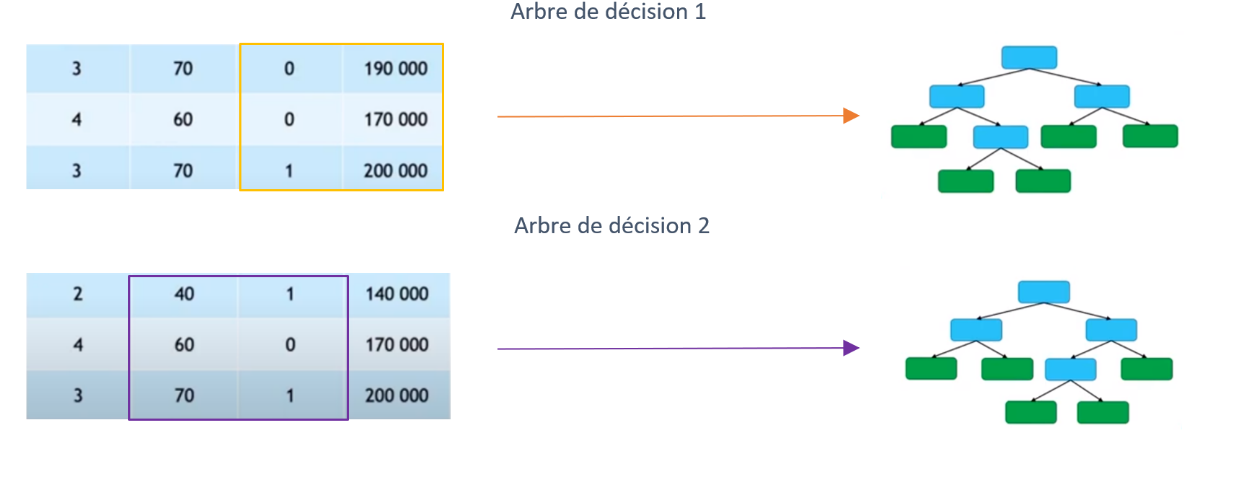
\includegraphics[width=0.8\linewidth]{Images/Figure12} 

}

\caption{Schéma 2 de construction d’un arbre de décision en RF}\label{fig:12}
\end{SCfigure}

\normalsize

La troisième étape consiste à répéter l'étape 1 et 2 afin de créer autant d'arbre de décision que l'on souhaite dans le but d'obtenir un ensemble (forêt) d'arbres de décision générés aléatoirement (figure \ref{fig:13}) \autocite{moutarde_arbres_2017}.
Le résultat de la RF va correspondre à la moyenne des décisions de l'ensemble des arbres pour l'élément recherché.

\scriptsize

\begin{SCfigure}

{\centering 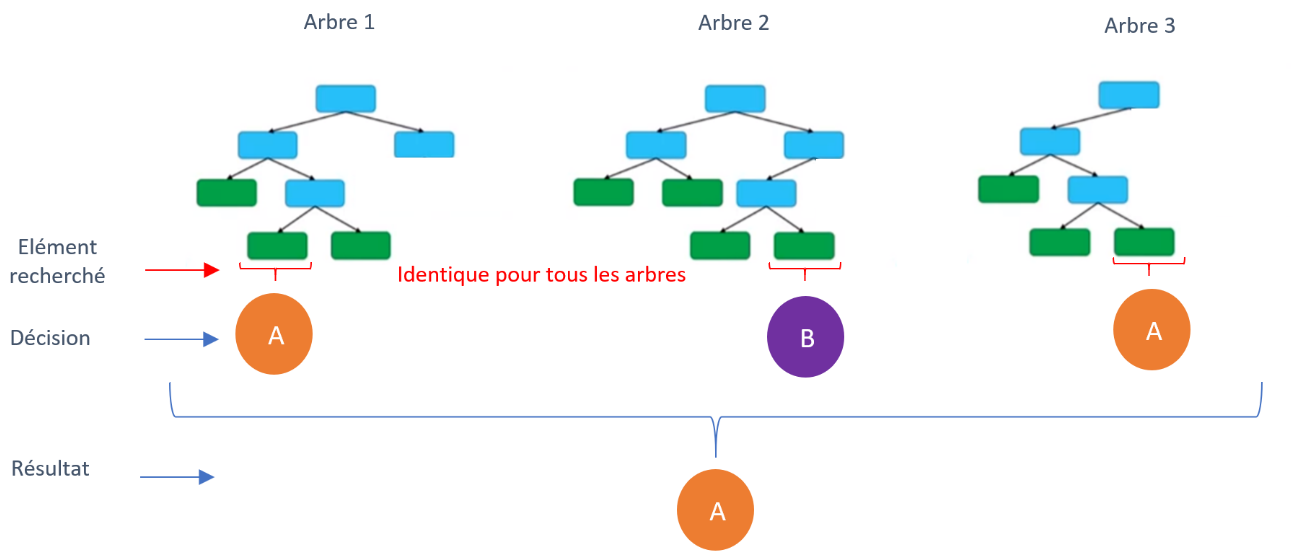
\includegraphics[width=0.8\linewidth]{Images/Figure13} 

}

\caption{Schéma de construction d’une Forêts Aléatoire}\label{fig:13}
\end{SCfigure}

\normalsize

\vfill
\newpage

\hypertarget{machine-uxe0-vecteurs-de-support-svm}{%
\section{Machine à Vecteurs de Support (SVM)}\label{machine-uxe0-vecteurs-de-support-svm}}

La SVM est aussi un algorithme d'apprentissage supervisé qui permet de faire des prédictions sur des variables qualitatives ou quantitatives \autocite{e1071}. L'objectif du SVM va consister à séparer deux classes de données, ici (infecté ; sain) pour pouvoir ensuite établir une généralisation dans la prédiction quand on ne connaîtra pas la nature de l'échantillon (infecté ; sain). Pour séparer ces deux classes, l'idée est de maximiser les distances entre les échantillons avec un hyperplan séparateur (appelé aussi « support vector ») (figure \ref{fig:14}) \autocite{cortes_support-vector_1995}.

\scriptsize

\begin{SCfigure}

{\centering 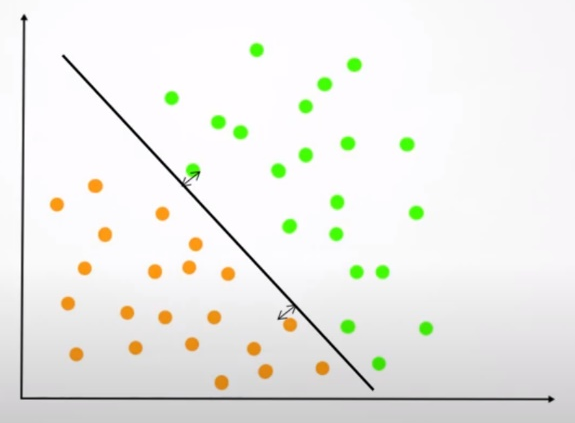
\includegraphics[width=0.8\linewidth]{Images/Figure14} 

}

\caption{Schéma de construction d’un hyperplan dans le cadre du SVM}\label{fig:14}
\end{SCfigure}

\normalsize

L'apprentissage supervisé va permettre de déterminer l'équation de l'hyperplan qui séparera les jeux de données des individus sains de ceux des malades. Cela va ensuite permettre la prédiction pour les jeux de données à tester.

\vfill
\newpage

\hypertarget{ruxe9gression-par-les-moindres-carruxe9s-partiels-pls}{%
\section{Régression par les Moindres Carrés Partiels (PLS)}\label{ruxe9gression-par-les-moindres-carruxe9s-partiels-pls}}

Pour finir la PLS est une méthode statistique permettant de traiter une variable binaire à expliquer (ici le statut HLB infecté ou sain) à partir de variables explicatives nombreuses (ici les mesures de réflectance pour chaque longueur d'onde) \autocite{pls}.

L'idée derrière la régression PLS est de créer, à partir d'un tableau avec n observations (les statuts HLB) décrites par X variables explicatives (réflectances pour chaque longueur d'onde), un ensemble de h composantes correspondant aux fonctions de chaque réflectance \autocite{tenehaus_lapproche_1999}.

Cette méthode consiste à rechercher dans un premier temps des composantes h, expliquant au mieux à la fois les variables explicatives X et les variables à expliquer Y. Les équations de régression PLS sont ensuite obtenues en régressant chaque variable Y sur les composantes h, puis en exprimant ces régressions en fonction des variables X d'origine (figure \ref{fig:15}) \autocite{tenehaus_lapproche_1999}.

\scriptsize

\begin{SCfigure}

{\centering 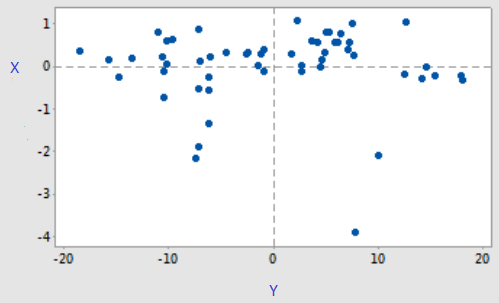
\includegraphics[width=0.8\linewidth]{Images/Figure15} 

}

\caption{Tableau représentant les coefficients de régression en fonction de X et Y}\label{fig:15}
\end{SCfigure}

\normalsize

Par conséquent, les coefficients de régression (les points bleus) sont positifs, nuls ou négatifs selon
que les vecteurs du plan représentant les variables X et Y forment un angle aigu, droit ou obtus.

L'apprentissage supervisé va permettre de déterminer les équations de régression PLS nécessaire à prédire les jeux de données à tester.

\vfill
\newpage

\hypertarget{performance-des-classifications}{%
\section{Performance des classifications}\label{performance-des-classifications}}

En apprentissage supervisé la matrice de confusion mesure la qualité d'un système de prédiction (table \ref{tab:MC}).

\scriptsize

\begin{longtable}[t]{lll}
\caption{\label{tab:MC}Matrice de confusion}\\
\toprule
  & Négatif confirmé & Positif confirmé\\
\midrule
Négatif prédit & Vrai Négatif (VN) & Faux Négatif (FN) (Erreur de type 2)\\
Positif prédit & Faux positif (FP) (Erreur de type 1) & Vrai positif (VP)\\
\bottomrule
\end{longtable}

\normalsize

De cette matrice, plusieurs paramètres de performance sont calculés dont :

\begin{itemize}
\item
  La qualité de la prédiction (Accuracy) = VP + VN / VP + VN + FN + FP met en évidence les erreurs de la prédiction qu'elles soient de type 1 ou de Type 2
\item
  La précision (Precision) = VP / VP + VP met en évidence les erreurs de type 1
\end{itemize}

L'erreur de type 1 est problématique dans le cadre de la maladie, car elle implique l'arrachage d'un arbre sain alors prédit comme étant positif au HLB

\begin{itemize}
\tightlist
\item
  La sensibilité (Sensitivity) = VP / VP + FN met en évidence les erreurs de type 2
\end{itemize}

L'erreur de type 2 impacte quant à elle la détection de la maladie, l'arbre est prédit comme étant négatif à la maladie alors qu'il est en réalité malade.

Ces paramètres permettent de rendre compte de l'efficacité de la prédiction et de pouvoir choisir la meilleure méthode de prédiction.

Ces méthodes ont été choisies à partir de la bibliographie où la qualité de la prédiction (Accuracy) est par exemple de 85\% pour SVM dans l'article de Sindhuja Sankaran \autocite{sankaran_huanglongbing_2013} et 96.4\% pour PLS dans l'article de Xiaoling Deng \autocite{deng_detection_2020}.

\hypertarget{amuxe9lioration-du-protocole-de-terrain}{%
\section{Amélioration du protocole de terrain}\label{amuxe9lioration-du-protocole-de-terrain}}

Afin d'améliorer le protocole de terrain pour de futures analyses, la question de savoir s'il était possible d'alléger le protocole de SPIR à main (i.e., faire moins de feuilles par arbre, moins de mesures de réflectance par feuille) sans perdre en performances de classification s'est posée. Pour ce faire, 100 jeux de données ont été simulés et dégradés par rééchantillonnage dans le vrai jeu de données et analysés avec les trois méthodes statistiques présentées.

\hypertarget{ruxe9sultats}{%
\chapter{Résultats}\label{ruxe9sultats}}

\hypertarget{influence-du-lieu-duxe9chantillonnage-et-des-variuxe9tuxe9s-sur-le-spectre-de-ruxe9flectance-global}{%
\section{Influence du lieu d'échantillonnage et des variétés sur le spectre de réflectance global}\label{influence-du-lieu-duxe9chantillonnage-et-des-variuxe9tuxe9s-sur-le-spectre-de-ruxe9flectance-global}}

Dans un premier temps, il est intéressant d'observer les données brutes des spectres de réflectance en fonction de leurs variétés.
La figure 2.1 montre les spectres de réflectance moyens des variétés citron (en vert), tangor (en orange) et zanzibar (en violet) (figure \ref{fig:19}).

\scriptsize

\begin{SCfigure}

{\centering \includegraphics[width=0.8\linewidth]{Rapport-Edouard_files/figure-latex/19-1} 

}

\caption{Spectre moyen en fonction de la variété pour les arbres négatifs aux HLB}\label{fig:19}
\end{SCfigure}

\normalsize

Les spectres des variétés échantillonnées ne semblent pas avoir de comportements significativement différents suivant les variétés sur l'ensemble des longueurs d'onde. L'analyse de ces données brutes ne suffit donc pas à renseigner sur l'influence que peuvent avoir les variétés sur les spectres du statut HLB.

Le calcul du F de Fisher via l'ANOVA est donc mis en œuvre afin de montrer un effet potentiel du lieu d'échantillonnage et des variétés sur le spectre de réflectance global (figure \ref{fig:x}).

\scriptsize

\begin{SCfigure}

{\centering \includegraphics[width=0.8\linewidth]{Rapport-Edouard_files/figure-latex/x-1} 

}

\caption{Valeur du F de Fisher pour chaque longueur d’onde montrant l’influence du facteur variété sur le spectre de réflectance global}\label{fig:x}
\end{SCfigure}

\normalsize

\vfill
\newpage

L'influence des variétés sur les spectres de réflectance est importante à partir de 1400nm avec un maximum à 1420nm (valeur F = 230). Ce maximum est suivi de deux autres pics à F = 200 à 1800nm et 2300nm, tous compris dans la partie du spectre correspondant aux infrarouges courtes longueurs d'onde.

Concernant l'influence de la parcelle sur le spectre de réflectance global, celle-ci a une forte influence (figure \ref{fig:y}).

\scriptsize

\begin{SCfigure}

{\centering \includegraphics[width=0.8\linewidth]{Rapport-Edouard_files/figure-latex/y-1} 

}

\caption{Valeur du F de Fisher pour chaque longueur d’onde montrant l’influence du facteur parcelle sur le spectre de réflectance global}\label{fig:y}
\end{SCfigure}

\normalsize

Dans le ``Red edge'' avec un maximum à 771nm (valeur F = 875) et une influence qui reste assez élevé (autour de F = 625) autour des longueurs d'onde 1500nm et 2100nm.

\vfill
\newpage

\hypertarget{effet-du-statut-hlb-sur-les-spectres-de-ruxe9flectance}{%
\section{Effet du statut HLB sur les spectres de réflectance}\label{effet-du-statut-hlb-sur-les-spectres-de-ruxe9flectance}}

La répartition des différentes variétés dans le jeu de données en fonction de leurs statuts HLB est assez équilibrée (table \ref{tab:T1}).

\scriptsize

\begin{longtable}[t]{lr}
\caption{\label{tab:T1}Répartition des variétés dans le jeu de données}\\
\toprule
Citron.Negatif & 25\\
Citron.Positif & 24\\
Tangor.Negatif & 23\\
Tangor.Positif & 23\\
Zanzibar.Negatif & 25\\
\addlinespace
Zanzibar.Positif & 20\\
Total & 140\\
\bottomrule
\end{longtable}

\normalsize

La figure 2.4 montre les spectres de réflectance moyens des arbres positifs au HLB (en rouge) et des arbres négatifs (en vert). On voit des différences nettes de spectre en fonction du statut HLB (figure \ref{fig:16}).

\scriptsize

\begin{SCfigure}

{\centering \includegraphics[width=0.8\linewidth]{Rapport-Edouard_files/figure-latex/16-1} 

}

\caption{Spectre moyen en fonction du statut HLB des arbres}\label{fig:16}
\end{SCfigure}

\normalsize

Sur certaines parties du spectre des différences de réflectance apparaissent encore plus nettement (figure \ref{fig:17}).

\scriptsize

\begin{SCfigure}

{\centering \includegraphics[width=0.8\linewidth]{Rapport-Edouard_files/figure-latex/17-1} 

}

\caption{Spectres individuels d’arbres positifs (en rouge) et négatifs (en vert) au HLB pour les longueurs d'onde de 400 à 680 nm}\label{fig:17}
\end{SCfigure}

\normalsize

Sur les longueurs d'onde de 400 à 680 nm les arbres positifs au HLB ont une réflectance légèrement plus élevée que les arbres sains.

Par ailleurs, une séparation moins nette s'observe dans la tranche de longueurs d'onde comprise entre 700 et 1400 nm (figure \ref{fig:18}).

\scriptsize

\begin{SCfigure}

{\centering \includegraphics[width=0.8\linewidth]{Rapport-Edouard_files/figure-latex/18-1} 

}

\caption{Spectres individuels d’arbres positifs (en rouge) et négatifs (en vert) au HLB pour les longueurs d’onde de 700 à 1400 nm}\label{fig:18}
\end{SCfigure}

\normalsize

La différence qui paraissait importante sur la figure 2.1 est à nuancer si l'on s'intéresse aux spectres individuels. En effet, il ne semble pas se dégager de tendance claire vis à vis du statut sur cette partie du spectre.

C'est pourquoi il est difficile d'affirmer avec certitude l'effet de la maladie sur les spectres de réflectance en fonction du statut HLB en utilisant seulement les données brutes.

Ainsi, il est intéressant de savoir s'il y a une influence de la maladie sur les spectres de réflectance et sur quelles longueurs d'onde se situe cet effet (figure \ref{fig:21}).

\scriptsize

\begin{SCfigure}

{\centering \includegraphics[width=0.8\linewidth]{Rapport-Edouard_files/figure-latex/21-1} 

}

\caption{Valeur du F de Fisher montrant l’influence du statut seul en interaction avec la variété sur le spectre de réflectance}\label{fig:21}
\end{SCfigure}

\normalsize

Globalement le statut HLB affecte le spectre de réflectance dans trois zones du spectre : dans le début du ``Red edge'' autour de 700nm, dans le proche infra-rouge autour de 800nm et dans le ``Short-wave infrared'' autour de 2000 nm avec un pic à 2032nm (valeur F = 751). Les effets du statut sont influencés dans le ``Red edge'' et le proche infra-rouge par le type de variété sur laquelle les feuilles ont été prélevées. Cependant le pic de cette influence correspond à une zone où la valeur de Fisher est quasi nulle pour l'effet du statut sur la détection de la maladie par la réflectance. Cette influence des variétés est donc comprise entre les valeurs de Fisher de 200 à 150 en excluant la zone de creux. Ces valeurs sont assez faibles si on les compare aux effets du statut qui avoisine les 700 et plus. Les trois variétés ont donc un impact plutôt faible sur la détection de la maladie via la mesure de la réflectance. Cet impact est encore plus minime (valeur F = 30) au niveau du pic d'influence de la maladie à 2032nm correspondant à la quantité d'eau dans la feuille. Cet impact est encore plus faible pour l'influence de la parcelle sur le statut HLB. Celle-ci n'a qu'une très faible influence sur le statut HLB au niveau des spectres dans visible et le ``Red edge'' (valeur F = 98) et une influence quasi nulle dans les autres longueurs d'onde

\vfill
\newpage

\hypertarget{lapproche-par-arbre-de-duxe9cision}{%
\section{L'approche par arbre de décision}\label{lapproche-par-arbre-de-duxe9cision}}

Une autre approche pour mettre en évidence l'effet du statut sur la détection de la maladie par la réflectance est la représentation en arbres de décision (figure \ref{fig:22}).

\scriptsize

\begin{SCfigure}

{\centering \includegraphics[width=0.8\linewidth]{Rapport-Edouard_files/figure-latex/22-1} 

}

\caption{Arbre de décision sur la réflectance des données globales par rapport au statut HLB}\label{fig:22}
\end{SCfigure}

\normalsize

Cette autre approche apporte des résultats identiques à la valeur de Fisher sur les longueurs d'onde où le statut HLB a le plus d'influence. Le premier nœud de décision à la longueur d'onde 2000nm est très significatif (p value 1.32e-36) et se divise entre les zones du ``Red edge'' à 706nm pour 774 feuilles et du proche-infra rouge à 1075nm pour les 666 feuilles restantes. Sur les 774 feuilles du deuxième nœud (p value 9.71e-18), 572 sont des feuilles issues d'arbres négatifs aux HLB à plus de 75\% environ en additionnant la part des effectifs négatifs des nœuds 6 et 7. Par ailleurs sur les 666 feuilles du nœud 9 (p value 4.84e-9), 333 sont globalement issus d'arbres positifs aux HLB à plus de 75\% environ en additionnant la part des effectifs positifs des nœuds 10 et 13. Cela montre qu'il est possible d'identifier depuis le spectre de réflectance, les arbres sains et malades avec un taux d'erreur d'environ 75\%.
L'intérêt de cette méthode en plus de donner les longueurs d'onde discriminantes pour la maladie, est la valeur de réflectance pour laquelle chaque longueur d'onde discriminante est clivante.

Enfin, en prenant uniquement la longueur d'onde la plus clivante (2000nm) selon l'arbre de décision, il est possible de se rendre compte de l'hétérogénéité des distributions à l'intérieur de celle-ci (figure \ref{fig:23}).

\scriptsize

\begin{SCfigure}

{\centering \includegraphics[width=0.8\linewidth]{Rapport-Edouard_files/figure-latex/23-1} 

}

\caption{Distribution des réflectances la longueur d’onde 2000nm}\label{fig:23}
\end{SCfigure}

\normalsize

\vfill
\newpage

Malgré l'échantillonnage différent selon les parcelles, les valeurs de réflectance sont normalement distribuées bien que centrées différemment. Chez Barret et Pothin, le centre est quasiment sur 0.09 alors que chez Gonthier et Hoarau celui-ci est environ à 0.07. Concernant les variétés, les Zanzibars semblent avoir les valeurs de réflectances les moins élevés. Malgré cette hétérogénéité dans la répartition des variables, qui est quasiment identique pour toutes les autres longueurs d'onde, cela n'a finalement pas un énorme impact sur la discrimination de la réflectance en fonction du statut.

\vfill
\newpage

\hypertarget{comparaison-des-performances-des-3-muxe9thodes-de-pruxe9diction-du-statut-hlb-uxe0-partir-des-spectres-ruxe9flectance}{%
\section{Comparaison des performances des 3 méthodes de prédiction du statut HLB à partir des spectres réflectance}\label{comparaison-des-performances-des-3-muxe9thodes-de-pruxe9diction-du-statut-hlb-uxe0-partir-des-spectres-ruxe9flectance}}

Pour prédire le statut des arbres à partir des spectres de réflectance, les trois méthodes d'analyses statistiques en apprentissage supervisé sont mises en œuvre. Pour chacune de ces méthodes, les paramètres de performance sont mesurés (table \ref{tab:T2}) après 100 simulations en calculs parallèles présentés en annexes 2 et 3.

\scriptsize

\begin{longtable}[t]{lrr}
\caption{\label{tab:T2}Paramètres de performance du statut HLB par Régression par les Moindres Carrés Partiels}\\
\toprule
Paramètres de performance & Moyenne & Ecart type\\
\midrule
Accuracy PLS & 92.6 & 1.7\\
Accuracy RF & 76.4 & 2.3\\
Accuracy SVM & 85.8 & 2.7\\
Precision PLS & 97.2 & 3.1\\
Precision RF & 88.3 & 3.1\\
\addlinespace
Precision SVM & 86.6 & 3.6\\
Sensitivity PLS & 88.3 & 2.7\\
Sensitivity RF & 60.7 & 4.8\\
Sensitivity SVM & 86.3 & 3.3\\
\bottomrule
\end{longtable}

\normalsize

Au vu de ces simulations, la méthode de régression par les moindres carrés partiels (PLS) est la plus robuste avec une qualité de prédiction (Accuracy) avoisinant les 92.6\% et avec l'écart type le plus faible d'environ 1.7.
Cette méthode est aussi très robuste pour minimiser les erreurs de type 1 (précision à 97.2\%) et de type 2 (sensibilité à 88.3\%) avec là aussi des écarts types plus faible que les deux autres méthodes.
Vient ensuite la méthode de la machine à vecteurs de support (SVM) avec une qualité de prédiction (Accuracy) d'environ 85.8\% et avec l'écart type le plus élevé avoisinant les 2.7. La méthode des forêts aléatoires (RF) est la moins robuste avec une qualité de prédiction (Accuracy) de 76.4\% approximativement.

\vfill
\newpage

\hypertarget{pruxe9diction-du-statut-hlb-par-ruxe9gression-par-les-moindres-carruxe9s-partiels-pls}{%
\section{Prédiction du statut HLB par Régression par les Moindres Carrés Partiels (PLS)}\label{pruxe9diction-du-statut-hlb-par-ruxe9gression-par-les-moindres-carruxe9s-partiels-pls}}

Concrètement, en utilisant la meilleure méthode, qui est celle des moindres carrés partiels, le statut des arbres peut donc être prédit précisément (figure \ref{fig:24}).

\scriptsize

\begin{SCfigure}

{\centering \includegraphics[width=0.8\linewidth]{Rapport-Edouard_files/figure-latex/24-1} 

}

\caption{Prédiction du statut HLB par Régression par les Moindres Carrés Partiels}\label{fig:24}
\end{SCfigure}

\normalsize

Cette représentation graphique est une aide à la décision afin de connaître le degré de précision de la prédiction sur chaque arbre. La prédiction par PLS donne une valeur correspondant à la moyenne des statuts prédits (compris entre 0 et 1 en ordonnés) des dix feuilles d'un arbre pour chaque arbre (en abscisse). Cela indique pour chaque arbre s'il est plutôt positif ou négatif, mais ça ne permet pas de trancher sur le statut de l'arbre. Cette prédiction se base donc sur deux seuils choisis via les observations de prédiction effectuées. Ces seuils sont compris entre 0.4 pour les arbres positifs qui seraient au-dessus de cette valeur (en rouge), 0.35 pour les arbres négatifs qui serait en dessous de cette valeur (en vert) et les arbres indéterminés (en gris) qui seraient compris entre ces deux valeurs. Une comparaison entre le statut réel des arbres est confirmé par qPCR (avec un croix pour les négatifs et un rond pour les positifs), permet ensuite de réaliser la matrice de confusion (table \ref{tab:T3})

\vfill
\newpage

\scriptsize

\begin{longtable}[t]{lrr}
\caption{\label{tab:T3}Matrice de confusion de la méthode de Régression par les Moindres Carrés Partiels}\\
\toprule
  & Négatif confirmé & Positif confirmé\\
\midrule
Négatif prédit & 57 & 2\\
Positif prédit & 10 & 62\\
\bottomrule
\end{longtable}

\normalsize

Sur cette prédiction, 62 arbres ont été prédits correctement positifs et 57 correctement négatifs. 10 arbres ont été prédits comme faussement positif (erreur de type 1) et 2 comme faussement négatif (erreur de type 2).

\scriptsize

\begin{longtable}[t]{lr}
\caption{\label{tab:T4}Paramètres de performance du statut HLB par Régression par les Moindres Carrés Partiels}\\
\toprule
Accuracy & 90.8\\
Precision & 96.6\\
Sensitivity & 85.1\\
\bottomrule
\end{longtable}

\normalsize

La prédiction par la méthode de régression par PLS a l'avantage d'avoir une précision élevée (96.6\%) ce qui minimise les erreurs de type 2, ce qui est très utile pour l'identification de la maladie sur une parcelle (table \ref{tab:T4}).

\vfill
\newpage

\hypertarget{amuxe9lioration-du-protocole-de-terrain-pour-le-choix-du-nombre-de-feuilles-par-arbre}{%
\section{Amélioration du protocole de terrain pour le choix du nombre de feuilles par arbre}\label{amuxe9lioration-du-protocole-de-terrain-pour-le-choix-du-nombre-de-feuilles-par-arbre}}

La méthode de la SVM est la méthode dont l'estimation des performances est la plus rapide à exécuter. Elle est donc utilisée pour tester s'il est possible d'alléger le protocole d'échantillonnage (figure \ref{fig:25}).

\scriptsize

\begin{SCfigure}

{\centering \includegraphics[width=0.8\linewidth]{Rapport-Edouard_files/figure-latex/25-1} 

}

\caption{Prédiction des paramètres de SVM en fonction du nombre de feuilles échantillonnés sur chaque arbre, obtenu après avoir fait la moyenne de 1000 SVM}\label{fig:25}
\end{SCfigure}

\normalsize

Après 1000 simulations, les paramètres de performance de la méthode SVM sont respectivement de 95\% pour la précision (Precision), 96\% pour la sensibilité (Sensitivity) et 97\% pour la qualité globale de la prédiction (Accuracy) pour un échantillonnage de 10 feuilles. La précision et la sensibilité passent en dessous des 90\% avec 5 feuilles prélevées. Avec 8 feuilles échantillonnées la qualité de la prédiction ainsi que la sensibilité ne baissent pas en dessous de 95\%.

\vfill
\newpage

\hypertarget{amuxe9lioration-du-protocole-de-terrain-pour-le-choix-du-nombre-de-mesures-de-ruxe9flectance-par-feuille}{%
\section{Amélioration du protocole de terrain pour le choix du nombre de mesures de réflectance par feuille}\label{amuxe9lioration-du-protocole-de-terrain-pour-le-choix-du-nombre-de-mesures-de-ruxe9flectance-par-feuille}}

\scriptsize

\begin{SCfigure}

{\centering \includegraphics[width=0.8\linewidth]{Rapport-Edouard_files/figure-latex/26-1} 

}

\caption{Prédiction des paramètres de SVM en fonction du nombre de répétition SPIR par feuille échantillonnés sur chaque arbre, obtenu après avoir fait la moyenne de 100 SVM}\label{fig:26}
\end{SCfigure}

\normalsize

Après 100 simulations, les paramètres de performances de la méthode SVM sont respectivement de 85\% pour la sensibilité (Sensitivity), 82\% pour la qualité globale de la prédiction (Accuracy) et 81\% pour la précision (Precision) pour un passage de 6 répétitions SPIR (figure \ref{fig:26}). Les écarts types étant assez marqués, au bout de 3 répétitions SPIR les paramètres de performance sont très peu changeants.

\vfill
\newpage

\hypertarget{discussion}{%
\chapter{Discussion}\label{discussion}}

Au vu des résultats, de part une valeur F de Fisher élevée (plus de 500 en moyenne), le lieu d'échantillonnage semble avoir un influence significative sur les valeurs de réflectance de 750 à 2500nm (figure \ref{fig:x}). Dans une moindre mesure, la variété à aussi une influence sur les valeurs de réflectance de 1400 à 2500nm avec une valeur F de Fisher de 150 en moyenne (figure \ref{fig:y}). Aucun de ces deux paramètres ne semble affecter les longueurs d'onde dans le visible de 350 à 700nm et les effet des variétés et du lieu d'échantillonnage sur le statut sont assez négligeable sur cette zone et dans l'infrarouge courte longueur d'onde (de 1400 à 2500nm).
Le statut seul a donc une influence sur cette partie du spectre avec une influence modérée des variétés et du lieu d'échantillonnage (figure \ref{fig:21}). Ainsi, dans le visible et le début du ``Red edge'', cette influence peut s'expliquer par une moins bonne absorbance de la lumière par la chlorophylle des feuilles à cause de la maladie.
Dans le proche infra-rouge autour de 800nm le statut a aussi une influence importante sur la réflectance avec en parallèle une influence importante du lieu d'échantillonnage sur cette partie du spectre (figure \ref{fig:y}).
Le proche infra-rouge correspondant à la structure interne de la feuille a un effet sur le spectre de réflectance global dû à la maladie. En effet, le HLB affect la structure cellulaire et en particulier celle du phloème, là où la bactérie se développe. Celle-ci va entraîner des nécroses et obstruer les vaisseaux. Ces dégradations vont donc altérer la réflectance de la lumière de cette partie de la feuille ce qui se voit lors de l'analyse des spectres.
Pour finir, c'est dans l'infrarouge courte longueur d'onde autour de 2000nm que s'observe la plus grande valeur F de Fisher (figure \ref{fig:21}) mais c'est aussi une zone du spectre où le lieu d'échantillonnage (figure \ref{fig:y}) et les variétés (figure \ref{fig:x}) dans une moindre mesure ont un effet sur la réflectance globale. L'effet du statut sur cette zone peut s'expliquer par une moins bonne absorbance de la lumière par la chlorophylle des feuilles en lien avec la maladie (figure \ref{fig:17}).
L'effet du statut sur cette zone peut s'expliquer par le fait que le HLB affecte grandement l'alimentation en eau de la feuille par l'obstruction des vaisseaux \autocite{bove_huanglongbing_2006}.

En plus de l'approche par la variance via l'ANOVA, l'approche par arbre de décision a permis de mettre en évidence d'une autre manière les longueurs d'onde discriminantes les plus clivantes. Ainsi, au vu de ces deux approches pour détecter plus facilement la maladie, 3 tranches de longueurs d'onde sont à favoriser, autour de 700nm, 1000nm et 2000nm (figure \ref{fig:22}). Ces longueurs d'onde trouvées sont similaires à celles présentes dans la documentation pour la détection du HLB \autocite{mishra_spectral_2007}.

La réalisation d'un modèle de prédiction du statut HLB par arbres à partir du spectre de réflectance s'est révélée être pertinente à bien des égards.
Le modèle de prédiction a permis de connaître l'état sanitaire des arbres via 3 méthodes d'analyse des spectres de réflectance. Ces 3 méthodes ont des qualités de prédiction (Accuracy) qui varie de 92.6\% pour la méthode PLS à 85.8\% et 76.4\% pour la méthode SVM et RF (table \ref{tab:T2}). Ces valeurs sont là aussi proches de celles présentes dans la bibliographie concernant la qualité de la prédiction avec 85\% pour SVM dans l'article de Sindhuja Sankaran \autocite{sankaran_huanglongbing_2013} et 96.4\% pour PLS dans l'article de Xiaoling Deng \autocite{deng_detection_2020}.
La méthode PLS étant la meilleure, elle permet de minimiser les erreurs de type 2 pour une meilleure identification de la maladie sur les parcelles (table \ref{tab:T2}). Cela peut s'expliquer dans la mesure où l'un des principaux intérêts de l'algorithme PLS est d'augmenter en performance et en fiabilité proportionnellement avec l'augmentation du nombre de variables explicatives permettant de prédire les composantes du modèle. C'est donc la méthode PLS qui est à favoriser pour les prédictions du statut HLB.

\vfill
\newpage

Finalement, cette étude confirme le haut potentiel qu'offre l'utilisation de la Spectroscopie Proche Infrarouge via une classification par PLS et SVM avec une approche orientée à la feuille pour la caractérisation de l'infection au HLB.
Cette caractérisation est possible grâce aux seuils de décision trouvés. Ces 2 seuils sont de 0.4 et plus pour les arbres malades à 0.35 et moins pour les arbres sains avec une classe indéterminée entre ces deux seuils.
Ces analyses ont aussi permis d'améliorer le protocole de terrain en préconisant un échantillonnage minimal de 8 feuilles par arbres (figure \ref{fig:25}) et 3 répétitions SPIR par feuille (figure \ref{fig:26}) pour un bon compromis entre le temps d'échantillonnage et la précision du modèle. L'utilisation de la proxidétection dans la surveillance du HLB doit tout de même être couplée à un travail de terrain avec analyse en qPCR pour la validation du statut des arbres.

Le modèle de prédiction réalisée dans ce rapport pourra, à terme, être utilisé comme un outil de détection décisif dans l'amélioration de surveillance épidémiologique du Huanglongbing (HLB) à La Réunion. Surtout si le modèle est alimenté avec de nouveaux échantillons dans le but d'agrandir la base d'apprentissage. En effet, ce modèle est pour l'instant valable uniquement pour 3 variétés d'agrumes sur les 27 que compte la Réunion. Afin d'optimiser ce modèle, il serait intéressant de l'enrichir avec d'avantage de variétés sur des lieux d'échantillonnages différents. Cela permettrait de répéter les analyses effectuées en comparant les résultats et les performances des différentes méthodes d'apprentissage supervisés testés pour améliorer le modèle.

\hypertarget{conclusion}{%
\chapter{Conclusion}\label{conclusion}}

Face à la résurgence actuelle du HLB à la Réunion, le potentiel d'un diagnostic HLB par SPIR, à la fois rapide que les analyses en laboratoire et peu onéreux est prometteur.

La construction de ce modèle de détection permettra de prédire le statut HLB des arbres sur différentes parcelles et d'en évaluer l'efficacité. Ce modèle permettra d'accentuer l'effort de surveillance sur les foyers de production les plus à risque où un échantillonnage qPCR classique n'est pas envisageable à grande échelle au regard des ressources disponibles.
Le modèle pouvant déterminer assez précisément quels arbres sont infectés au HLB au sein d'une parcelle, cela permettra d'accompagner au mieux les agriculteurs dans la lutte contre la maladie.

Ainsi, prédire le statut HLB des parcelles d'agrumes par apprentissage supervisé est une solution prometteuse bien que la base de données d'apprentissage doit être étoffée pour garantir une prédiction plus juste à long terme.

\hypertarget{annexe}{%
\chapter{Annexe}\label{annexe}}

Pour l'utilisation des différents packages :

\begin{itemize}
\tightlist
\item
  Pour la facilité d'installation et le chargement de plusieurs paquets : tidyverse \autocite{tidyverse}
\item
  Pour l'échantillonnage aléatoire : catools \autocite{caTools}
\item
  Pour la réalisation des graphiques : ggplot2 \autocite{ggplot2}
\item
  Pour la réalisation de l'arbre de décision : ggparty \autocite{ggparty}
\item
  Pour la manipulation du jeu de données :tidyr \autocite{tidyr}
\item
  Pour l'algorithme de calculs parallèles : snowfall \autocite{snowfall}
\end{itemize}

\scriptsize

\normalsize

\vfill
\newpage
\SmallMargins

\hypertarget{annexe-1-importation-des-donnuxe9es-brutes}{%
\section{Annexe 1 : Importation des données brutes}\label{annexe-1-importation-des-donnuxe9es-brutes}}

\scriptsize

\begin{Shaded}
\begin{Highlighting}[]
\SpecialCharTok{\textgreater{}} \FunctionTok{library}\NormalTok{(tidyr)  }\CommentTok{\# pivot longer \& pivot\_wider}
\SpecialCharTok{\textgreater{}} \CommentTok{\# Importation des donnees SPIR Global \#\#\#\#}
\ErrorTok{\textgreater{}}\NormalTok{ data\_SPIR\_Ed }\OtherTok{\textless{}{-}} \FunctionTok{read.table}\NormalTok{(}\AttributeTok{file =} \StringTok{"SPIR\_Global.csv"}\NormalTok{, }
\SpecialCharTok{+}     \AttributeTok{header =}\NormalTok{ T, }\AttributeTok{sep =} \StringTok{";"}\NormalTok{, }\AttributeTok{stringsAsFactors =}\NormalTok{ T, }\AttributeTok{row.names =} \DecValTok{1}\NormalTok{, }
\SpecialCharTok{+}     \AttributeTok{na.strings =} \FunctionTok{c}\NormalTok{(}\StringTok{""}\NormalTok{, }\StringTok{"NA"}\NormalTok{), }\AttributeTok{dec =} \StringTok{","}\NormalTok{)}
\SpecialCharTok{\textgreater{}} \CommentTok{\# Creation des colonne \textquotesingle{}code\textquotesingle{} de data\_SPIR\_Ed}
\ErrorTok{\textgreater{}}\NormalTok{ code\_labo }\OtherTok{\textless{}{-}} \FunctionTok{rownames}\NormalTok{(data\_SPIR\_Ed)}
\SpecialCharTok{\textgreater{}} \FunctionTok{names}\NormalTok{(data\_SPIR\_Ed)[}\DecValTok{1}\NormalTok{] }\OtherTok{=} \FunctionTok{c}\NormalTok{(}\StringTok{"code\_variete"}\NormalTok{)}
\SpecialCharTok{\textgreater{}} \FunctionTok{names}\NormalTok{(data\_SPIR\_Ed)[}\DecValTok{2}\NormalTok{] }\OtherTok{=} \FunctionTok{c}\NormalTok{(}\StringTok{"code\_agri"}\NormalTok{)}
\SpecialCharTok{\textgreater{}}\NormalTok{ data\_SPIR\_Ed}\SpecialCharTok{$}\NormalTok{code\_nbr\_rep }\OtherTok{\textless{}{-}} \FunctionTok{factor}\NormalTok{(}\FunctionTok{substr}\NormalTok{(code\_labo, }
\SpecialCharTok{+}     \DecValTok{8}\NormalTok{, }\DecValTok{8}\NormalTok{))}
\SpecialCharTok{\textgreater{}}\NormalTok{ data\_SPIR\_Ed}\SpecialCharTok{$}\NormalTok{code\_ech\_arbre }\OtherTok{\textless{}{-}} \FunctionTok{factor}\NormalTok{(}\FunctionTok{substr}\NormalTok{(code\_labo, }
\SpecialCharTok{+}     \DecValTok{1}\NormalTok{, }\DecValTok{2}\NormalTok{))}
\SpecialCharTok{\textgreater{}}\NormalTok{ data\_SPIR\_Ed}\SpecialCharTok{$}\NormalTok{code\_ech\_feuille }\OtherTok{\textless{}{-}} \FunctionTok{factor}\NormalTok{(}\FunctionTok{substr}\NormalTok{(code\_labo, }
\SpecialCharTok{+}     \DecValTok{1}\NormalTok{, }\DecValTok{3}\NormalTok{))}
\SpecialCharTok{\textgreater{}}\NormalTok{ data\_SPIR\_Ed}\SpecialCharTok{$}\NormalTok{code\_rep\_feuille }\OtherTok{\textless{}{-}} \FunctionTok{factor}\NormalTok{(}\FunctionTok{paste}\NormalTok{(data\_SPIR\_Ed}\SpecialCharTok{$}\NormalTok{code\_ech\_feuille, }
\SpecialCharTok{+}\NormalTok{     data\_SPIR\_Ed}\SpecialCharTok{$}\NormalTok{code\_nbr\_rep, }\AttributeTok{sep =} \StringTok{""}\NormalTok{))}
\SpecialCharTok{\textgreater{}} \FunctionTok{rm}\NormalTok{(code\_labo)}
\SpecialCharTok{\textgreater{}}\NormalTok{ data\_SPIR\_Ed }\OtherTok{\textless{}{-}}\NormalTok{ data\_SPIR\_Ed[}\SpecialCharTok{!}\FunctionTok{is.na}\NormalTok{(data\_SPIR\_Ed}\SpecialCharTok{$}\NormalTok{X350), }
\SpecialCharTok{+}\NormalTok{     ]}
\SpecialCharTok{\textgreater{}} \CommentTok{\# Importation et preparation des resultats de la}
\ErrorTok{\textgreater{}} \CommentTok{\# Qpcr Globaux \#\#\#\#}
\ErrorTok{\textgreater{}}\NormalTok{ data\_Qpcr\_Ed }\OtherTok{\textless{}{-}} \FunctionTok{read.table}\NormalTok{(}\AttributeTok{file =} \StringTok{"qPCR\_global\_Ed.csv"}\NormalTok{, }
\SpecialCharTok{+}     \AttributeTok{header =}\NormalTok{ T, }\AttributeTok{sep =} \StringTok{";"}\NormalTok{, }\AttributeTok{stringsAsFactors =}\NormalTok{ T, }\AttributeTok{row.names =} \DecValTok{1}\NormalTok{, }
\SpecialCharTok{+}     \AttributeTok{na.strings =} \FunctionTok{c}\NormalTok{(}\StringTok{""}\NormalTok{, }\StringTok{"NA"}\NormalTok{), }\AttributeTok{dec =} \StringTok{","}\NormalTok{)}
\SpecialCharTok{\textgreater{}} \CommentTok{\# on stocke les noms d\textquotesingle{}echantillons positifs selon}
\ErrorTok{\textgreater{}} \CommentTok{\# nos 2 seuils de Ct (cycle de qPCR ), a savoir}
\ErrorTok{\textgreater{}} \CommentTok{\# moins de 32 cyclces et moins de 36 cycles qPCR}
\ErrorTok{\textgreater{}}\NormalTok{ seuils }\OtherTok{\textless{}{-}} \FunctionTok{c}\NormalTok{(}\DecValTok{32}\NormalTok{, }\DecValTok{36}\NormalTok{)}
\SpecialCharTok{\textgreater{}}\NormalTok{ trueP }\OtherTok{\textless{}{-}} \FunctionTok{lapply}\NormalTok{(seuils, }\ControlFlowTok{function}\NormalTok{(x) }\FunctionTok{unique}\NormalTok{(data\_Qpcr\_Ed}\SpecialCharTok{$}\NormalTok{Sample.Name[}\FunctionTok{which}\NormalTok{(data\_Qpcr\_Ed}\SpecialCharTok{$}\NormalTok{C..Mean }\SpecialCharTok{\textless{}} 
\SpecialCharTok{+}\NormalTok{     x }\SpecialCharTok{\&}\NormalTok{ data\_Qpcr\_Ed}\SpecialCharTok{$}\NormalTok{C..SD }\SpecialCharTok{\textless{}} \DecValTok{1}\NormalTok{)]))}
\SpecialCharTok{\textgreater{}} \FunctionTok{names}\NormalTok{(trueP) }\OtherTok{\textless{}{-}} \FunctionTok{paste}\NormalTok{(}\StringTok{"seuil"}\NormalTok{, seuils, }\AttributeTok{sep =} \StringTok{"."}\NormalTok{)}
\SpecialCharTok{\textgreater{}}\NormalTok{ data\_SPIR\_Ed[}\FunctionTok{paste}\NormalTok{(}\StringTok{"qPCR"}\NormalTok{, seuils, }\AttributeTok{sep =} \StringTok{"\_"}\NormalTok{)] }\OtherTok{\textless{}{-}} \FunctionTok{lapply}\NormalTok{(trueP, }
\SpecialCharTok{+}     \ControlFlowTok{function}\NormalTok{(x) }\FunctionTok{as.numeric}\NormalTok{(data\_SPIR\_Ed}\SpecialCharTok{$}\NormalTok{code\_ech\_arbre }\SpecialCharTok{\%in\%} 
\SpecialCharTok{+}\NormalTok{         x))}
\SpecialCharTok{\textgreater{}} \CommentTok{\# on cherche quels sont les code\_ech\_arbre qui se}
\ErrorTok{\textgreater{}} \CommentTok{\# trouvent dans le vecteur x x reprenant}
\ErrorTok{\textgreater{}} \CommentTok{\# automatiquement les noms des arbres positifs}
\ErrorTok{\textgreater{}} \CommentTok{\# selon le seuil choisi}
\ErrorTok{\textgreater{}}\NormalTok{ select.lambda }\OtherTok{\textless{}{-}} \FunctionTok{grep}\NormalTok{(}\StringTok{"\^{}X"}\NormalTok{, }\FunctionTok{names}\NormalTok{(data\_SPIR\_Ed))}
\SpecialCharTok{\textgreater{}}\NormalTok{ data\_SPIR\_Ed }\OtherTok{\textless{}{-}}\NormalTok{ data\_SPIR\_Ed[, }\FunctionTok{c}\NormalTok{(}\FunctionTok{names}\NormalTok{(data\_SPIR\_Ed)[}\SpecialCharTok{{-}}\NormalTok{select.lambda], }
\SpecialCharTok{+}     \FunctionTok{names}\NormalTok{(data\_SPIR\_Ed)[select.lambda])]}
\SpecialCharTok{\textgreater{}} \FunctionTok{rm}\NormalTok{(data\_Qpcr\_Ed, select.lambda, seuils)}
\SpecialCharTok{\textgreater{}}\NormalTok{ data\_SPIR\_Ed[}\FunctionTok{c}\NormalTok{(}\StringTok{"qPCR\_32"}\NormalTok{, }\StringTok{"qPCR\_36"}\NormalTok{)] }\OtherTok{\textless{}{-}} \FunctionTok{lapply}\NormalTok{(data\_SPIR\_Ed[}\FunctionTok{c}\NormalTok{(}\StringTok{"qPCR\_32"}\NormalTok{, }
\SpecialCharTok{+}     \StringTok{"qPCR\_36"}\NormalTok{)], factor)}
\SpecialCharTok{\textgreater{}} \CommentTok{\# Format\_long \#\#\#\#}
\ErrorTok{\textgreater{}}\NormalTok{ select.lambda }\OtherTok{\textless{}{-}} \FunctionTok{grep}\NormalTok{(}\StringTok{"\^{}X"}\NormalTok{, }\FunctionTok{names}\NormalTok{(data\_SPIR\_Ed))}
\SpecialCharTok{\textgreater{}}\NormalTok{ data\_long\_Ed }\OtherTok{\textless{}{-}} \FunctionTok{pivot\_longer}\NormalTok{(}\AttributeTok{data =}\NormalTok{ data\_SPIR\_Ed, }\AttributeTok{cols =}\NormalTok{ select.lambda, }
\SpecialCharTok{+}     \AttributeTok{values\_to =} \StringTok{"reflectance"}\NormalTok{, }\AttributeTok{names\_to =} \StringTok{"lambda"}\NormalTok{)}
\SpecialCharTok{\textgreater{}}\NormalTok{ data\_long\_Ed}\SpecialCharTok{$}\NormalTok{lambda }\OtherTok{\textless{}{-}} \FunctionTok{as.numeric}\NormalTok{(}\FunctionTok{gsub}\NormalTok{(}\StringTok{"X"}\NormalTok{, }\StringTok{""}\NormalTok{, data\_long\_Ed}\SpecialCharTok{$}\NormalTok{lambda))}
\SpecialCharTok{\textgreater{}}\NormalTok{ data\_long\_Ed }\OtherTok{\textless{}{-}}\NormalTok{ data\_long\_Ed[}\SpecialCharTok{!}\FunctionTok{is.na}\NormalTok{(data\_long\_Ed}\SpecialCharTok{$}\NormalTok{reflectance), }
\SpecialCharTok{+}\NormalTok{     ]}
\end{Highlighting}
\end{Shaded}

\normalsize

\vfill
\newpage

\hypertarget{annexe-2-fonction-matrice-de-confusion}{%
\section{Annexe 2 : Fonction Matrice de confusion}\label{annexe-2-fonction-matrice-de-confusion}}

\scriptsize

\begin{Shaded}
\begin{Highlighting}[]
\SpecialCharTok{\textgreater{}}\NormalTok{ fct\_ConfusionMatrix }\OtherTok{\textless{}{-}} \ControlFlowTok{function}\NormalTok{(nb.rep, seuil.ct, list.feuilles) \{}
\SpecialCharTok{+}\NormalTok{     maliste }\OtherTok{\textless{}{-}} \FunctionTok{lapply}\NormalTok{(list.feuilles, }\ControlFlowTok{function}\NormalTok{(feuille) \{}
\SpecialCharTok{+}\NormalTok{         list\_svm }\OtherTok{\textless{}{-}}\NormalTok{ feuille[}\FunctionTok{sample}\NormalTok{(}\DecValTok{1}\SpecialCharTok{:}\FunctionTok{length}\NormalTok{(feuille}\SpecialCharTok{$}\NormalTok{code\_ech\_feuille), }
\SpecialCharTok{+}\NormalTok{             nb.rep), ]}
\SpecialCharTok{+}         \CommentTok{\# on fait ça pour tte les feuilles mais tjrs en}
\SpecialCharTok{+}         \CommentTok{\# choisissant le nombre de rep tire aleatoirement}
\SpecialCharTok{+}\NormalTok{         code }\OtherTok{\textless{}{-}} \FunctionTok{grep}\NormalTok{(}\StringTok{"\^{}code\_ech"}\NormalTok{, }\FunctionTok{names}\NormalTok{(list\_svm))}
\SpecialCharTok{+}\NormalTok{         qPCR }\OtherTok{\textless{}{-}} \FunctionTok{grep}\NormalTok{(}\StringTok{"\^{}qPCR\_"}\NormalTok{, }\FunctionTok{names}\NormalTok{(list\_svm))}
\SpecialCharTok{+}\NormalTok{         sortie }\OtherTok{\textless{}{-}} \FunctionTok{cbind.data.frame}\NormalTok{(}\FunctionTok{unique}\NormalTok{(list\_svm[}\FunctionTok{c}\NormalTok{(code, }
\SpecialCharTok{+}\NormalTok{             qPCR)]), }\FunctionTok{matrix}\NormalTok{(}\FunctionTok{apply}\NormalTok{(list\_svm[}\SpecialCharTok{{-}}\NormalTok{(}\FunctionTok{which}\NormalTok{(}\FunctionTok{colnames}\NormalTok{(list\_svm) }\SpecialCharTok{==} 
\SpecialCharTok{+}             \StringTok{"code\_variete"}\NormalTok{)}\SpecialCharTok{:}\FunctionTok{which}\NormalTok{(}\FunctionTok{colnames}\NormalTok{(list\_svm) }\SpecialCharTok{==} 
\SpecialCharTok{+}             \StringTok{"qPCR\_36"}\NormalTok{))], }\DecValTok{2}\NormalTok{, mean), }\AttributeTok{nr =} \DecValTok{1}\NormalTok{, }\AttributeTok{dimnames =} \FunctionTok{list}\NormalTok{(}\ConstantTok{NULL}\NormalTok{, }
\SpecialCharTok{+}             \FunctionTok{names}\NormalTok{(list\_svm)[}\SpecialCharTok{{-}}\NormalTok{(}\FunctionTok{which}\NormalTok{(}\FunctionTok{colnames}\NormalTok{(list\_svm) }\SpecialCharTok{==} 
\SpecialCharTok{+}                 \StringTok{"code\_variete"}\NormalTok{)}\SpecialCharTok{:}\FunctionTok{which}\NormalTok{(}\FunctionTok{colnames}\NormalTok{(list\_svm) }\SpecialCharTok{==} 
\SpecialCharTok{+}                 \StringTok{"qPCR\_36"}\NormalTok{))])))}
\SpecialCharTok{+}\NormalTok{         sortie}
\SpecialCharTok{+}\NormalTok{     \})}
\SpecialCharTok{+}\NormalTok{     test\_ed }\OtherTok{\textless{}{-}} \FunctionTok{do.call}\NormalTok{(rbind, maliste)  }\CommentTok{\# on colle toute les listes créées précédement }
\SpecialCharTok{+}\NormalTok{     test\_ed }\OtherTok{\textless{}{-}}\NormalTok{ test\_ed[}\SpecialCharTok{{-}}\NormalTok{(}\FunctionTok{which}\NormalTok{(}\FunctionTok{colnames}\NormalTok{(test\_ed) }\SpecialCharTok{==} 
\SpecialCharTok{+}         \StringTok{"qPCR\_32"}\NormalTok{))]}
\SpecialCharTok{+}\NormalTok{     test\_ed[[}\FunctionTok{paste0}\NormalTok{(}\StringTok{"qPCR\_"}\NormalTok{, seuil.ct)]] }\OtherTok{\textless{}{-}} \FunctionTok{as.numeric}\NormalTok{(}\FunctionTok{as.character}\NormalTok{(test\_ed[[}\FunctionTok{paste0}\NormalTok{(}\StringTok{"qPCR\_"}\NormalTok{, }
\SpecialCharTok{+}\NormalTok{         seuil.ct)]]))}
\SpecialCharTok{+}\NormalTok{     decoup }\OtherTok{\textless{}{-}} \FunctionTok{sample.split}\NormalTok{(test\_ed[, }\FunctionTok{paste0}\NormalTok{(}\StringTok{"qPCR\_"}\NormalTok{, }
\SpecialCharTok{+}\NormalTok{         seuil.ct)], }\AttributeTok{SplitRatio =} \FloatTok{0.5}\NormalTok{)  }\CommentTok{\# on decoupe le jeu de donné en training set et test set}
\SpecialCharTok{+}\NormalTok{     training\_set }\OtherTok{\textless{}{-}}\NormalTok{ test\_ed[decoup, ]}
\SpecialCharTok{+}\NormalTok{     test\_set }\OtherTok{\textless{}{-}}\NormalTok{ test\_ed[}\SpecialCharTok{!}\NormalTok{decoup, ]}
\SpecialCharTok{+}     \CommentTok{\# Criteres choisi pour la separation des donnees}
\SpecialCharTok{+}\NormalTok{     crit.pos }\OtherTok{\textless{}{-}} \FloatTok{0.4}
\SpecialCharTok{+}\NormalTok{     crit.neg }\OtherTok{\textless{}{-}} \FloatTok{0.35}
\SpecialCharTok{+}\NormalTok{     trueP}\SpecialCharTok{$}\NormalTok{seuil}\FloatTok{.32} \OtherTok{\textless{}{-}} \ConstantTok{NULL}
\SpecialCharTok{+}     \CommentTok{\# Prediction RF \#\#\#\#}
\SpecialCharTok{+}\NormalTok{     model\_rf\_36 }\OtherTok{\textless{}{-}} \FunctionTok{randomForest}\NormalTok{(}\AttributeTok{x =}\NormalTok{ training\_set[, }
\SpecialCharTok{+}         \FunctionTok{grep}\NormalTok{(}\StringTok{"\^{}X"}\NormalTok{, }\FunctionTok{names}\NormalTok{(training\_set))], }\AttributeTok{y =}\NormalTok{ training\_set[[}\FunctionTok{paste0}\NormalTok{(}\StringTok{"qPCR\_"}\NormalTok{, }
\SpecialCharTok{+}\NormalTok{         seuil.ct)]], }\AttributeTok{ntree =} \DecValTok{100}\NormalTok{)}
\SpecialCharTok{+}     \CommentTok{\# Prediction sur les feuilles de la base}
\SpecialCharTok{+}     \CommentTok{\# d\textquotesingle{}apprentissage}
\SpecialCharTok{+}\NormalTok{     rf\_pred }\OtherTok{\textless{}{-}}\NormalTok{ test\_set}
\SpecialCharTok{+}\NormalTok{     rf\_pred}\SpecialCharTok{$}\NormalTok{rf\_pred\_36 }\OtherTok{\textless{}{-}} \FunctionTok{predict}\NormalTok{(model\_rf\_36, }\AttributeTok{newdata =}\NormalTok{ test\_set, }
\SpecialCharTok{+}         \AttributeTok{decision.values =}\NormalTok{ T)}
\SpecialCharTok{+}     \CommentTok{\# Conversion des resultats de la prediction en}
\SpecialCharTok{+}     \CommentTok{\# numerique}
\SpecialCharTok{+}\NormalTok{     rf\_pred}\SpecialCharTok{$}\NormalTok{rf\_pred\_36 }\OtherTok{=} \FunctionTok{as.numeric}\NormalTok{(}\FunctionTok{as.character}\NormalTok{(rf\_pred}\SpecialCharTok{$}\NormalTok{rf\_pred\_36))}
\SpecialCharTok{+}     \CommentTok{\# Moyennage des resultats de la prediction pour}
\SpecialCharTok{+}     \CommentTok{\# chaque arbres}
\SpecialCharTok{+}\NormalTok{     rf\_pred\_arbres\_36 }\OtherTok{=} \FunctionTok{aggregate}\NormalTok{(rf\_pred\_36 }\SpecialCharTok{\textasciitilde{}}\NormalTok{ code\_ech\_arbre, }
\SpecialCharTok{+}         \AttributeTok{data =}\NormalTok{ rf\_pred, mean, }\AttributeTok{na.rm =}\NormalTok{ T)}
\SpecialCharTok{+}\NormalTok{     rf\_pred\_arbres\_36}\SpecialCharTok{$}\NormalTok{crit }\OtherTok{\textless{}{-}} \FloatTok{0.5}
\SpecialCharTok{+}\NormalTok{     rf\_pred\_arbres\_36}\SpecialCharTok{$}\NormalTok{crit[rf\_pred\_arbres\_36}\SpecialCharTok{$}\NormalTok{rf\_pred\_36 }\SpecialCharTok{\textgreater{}=} 
\SpecialCharTok{+}\NormalTok{         crit.pos] }\OtherTok{\textless{}{-}} \DecValTok{1}
\SpecialCharTok{+}\NormalTok{     rf\_pred\_arbres\_36}\SpecialCharTok{$}\NormalTok{crit[rf\_pred\_arbres\_36}\SpecialCharTok{$}\NormalTok{rf\_pred\_36 }\SpecialCharTok{\textless{}=} 
\SpecialCharTok{+}\NormalTok{         crit.neg] }\OtherTok{\textless{}{-}} \DecValTok{0}
\SpecialCharTok{+}     \CommentTok{\# Creation d\textquotesingle{}une nouvelle colonne des resulats issu}
\SpecialCharTok{+}     \CommentTok{\# de la qPCR, pour comparer à la valeurs predite}
\SpecialCharTok{+}\NormalTok{     rf\_pred\_arbres\_36[}\FunctionTok{paste}\NormalTok{(}\StringTok{"qPCR"}\NormalTok{, seuil.ct, }\AttributeTok{sep =} \StringTok{"\_"}\NormalTok{)] }\OtherTok{\textless{}{-}} \FunctionTok{lapply}\NormalTok{(trueP, }
\SpecialCharTok{+}         \ControlFlowTok{function}\NormalTok{(x) }\FunctionTok{as.numeric}\NormalTok{(rf\_pred\_arbres\_36}\SpecialCharTok{$}\NormalTok{code\_ech\_arbre }\SpecialCharTok{\%in\%} 
\SpecialCharTok{+}\NormalTok{             x))}
\SpecialCharTok{+}     \CommentTok{\# Résultats de la prédiction sous forme de matrice}
\SpecialCharTok{+}     \CommentTok{\# de confusion}
\SpecialCharTok{+}\NormalTok{     rf\_pred\_arbres\_36}\SpecialCharTok{$}\NormalTok{crit }\OtherTok{\textless{}{-}} \FunctionTok{factor}\NormalTok{(rf\_pred\_arbres\_36}\SpecialCharTok{$}\NormalTok{crit, }
\SpecialCharTok{+}         \AttributeTok{levels =} \FunctionTok{c}\NormalTok{(}\DecValTok{0}\NormalTok{, }\DecValTok{1}\NormalTok{))}
\SpecialCharTok{+}\NormalTok{     rf\_confusion\_matrix\_36 }\OtherTok{\textless{}{-}} \FunctionTok{ftable}\NormalTok{(qPCR\_36 }\SpecialCharTok{\textasciitilde{}}\NormalTok{ crit, }
\SpecialCharTok{+}         \AttributeTok{data =}\NormalTok{ rf\_pred\_arbres\_36)}
\SpecialCharTok{+}\NormalTok{     rf\_confusion\_matrix\_36 }\OtherTok{\textless{}{-}} \FunctionTok{as.matrix}\NormalTok{(rf\_confusion\_matrix\_36)}
\SpecialCharTok{+}\NormalTok{     TP\_rf }\OtherTok{\textless{}{-}}\NormalTok{ rf\_confusion\_matrix\_36[}\DecValTok{1}\NormalTok{, }\DecValTok{1}\NormalTok{]}
\SpecialCharTok{+}\NormalTok{     TN\_rf }\OtherTok{\textless{}{-}}\NormalTok{ rf\_confusion\_matrix\_36[}\DecValTok{2}\NormalTok{, }\DecValTok{2}\NormalTok{]}
\SpecialCharTok{+}\NormalTok{     FN\_rf }\OtherTok{\textless{}{-}}\NormalTok{ rf\_confusion\_matrix\_36[}\DecValTok{2}\NormalTok{, }\DecValTok{1}\NormalTok{]}
\SpecialCharTok{+}\NormalTok{     FP\_rf }\OtherTok{\textless{}{-}}\NormalTok{ rf\_confusion\_matrix\_36[}\DecValTok{1}\NormalTok{, }\DecValTok{2}\NormalTok{]}
\SpecialCharTok{+}     \CommentTok{\# Calcul des parametres rf de la matrice de}
\SpecialCharTok{+}     \CommentTok{\# confusion}
\SpecialCharTok{+}\NormalTok{     Accuracy\_rf36 }\OtherTok{\textless{}{-}}\NormalTok{ ((TP\_rf }\SpecialCharTok{+}\NormalTok{ TN\_rf)}\SpecialCharTok{/}\NormalTok{(TP\_rf }\SpecialCharTok{+}\NormalTok{ TN\_rf }\SpecialCharTok{+} 
\SpecialCharTok{+}\NormalTok{         FN\_rf }\SpecialCharTok{+}\NormalTok{ FP\_rf) }\SpecialCharTok{*} \DecValTok{100}\NormalTok{)}
\SpecialCharTok{+}\NormalTok{     Precision\_rf36 }\OtherTok{\textless{}{-}}\NormalTok{ ((TP\_rf}\SpecialCharTok{/}\NormalTok{(TP\_rf }\SpecialCharTok{+}\NormalTok{ FP\_rf) }\SpecialCharTok{*} \DecValTok{100}\NormalTok{))}
\SpecialCharTok{+}\NormalTok{     Sensitivity\_rf36 }\OtherTok{\textless{}{-}}\NormalTok{ ((TP\_rf}\SpecialCharTok{/}\NormalTok{(TP\_rf }\SpecialCharTok{+}\NormalTok{ FN\_rf) }\SpecialCharTok{*} \DecValTok{100}\NormalTok{))}
\SpecialCharTok{+}\NormalTok{     Parametre\_rf\_36 }\OtherTok{\textless{}{-}} \FunctionTok{rbind}\NormalTok{(Accuracy\_rf36, Precision\_rf36, }
\SpecialCharTok{+}\NormalTok{         Sensitivity\_rf36)}
\SpecialCharTok{+}     \CommentTok{\# Prediction SVM \#\#\#\#}
\SpecialCharTok{+}\NormalTok{     model\_SVM\_36 }\OtherTok{\textless{}{-}} \FunctionTok{svm}\NormalTok{(}\AttributeTok{y =}\NormalTok{ training\_set[, }\FunctionTok{paste0}\NormalTok{(}\StringTok{"qPCR\_"}\NormalTok{, }
\SpecialCharTok{+}\NormalTok{         seuil.ct)], }\AttributeTok{x =}\NormalTok{ training\_set[, }\FunctionTok{grep}\NormalTok{(}\StringTok{"\^{}X"}\NormalTok{, }\FunctionTok{names}\NormalTok{(training\_set))], }
\SpecialCharTok{+}         \AttributeTok{type =} \StringTok{"C{-}classification"}\NormalTok{, }\AttributeTok{kernel =} \StringTok{"linear"}\NormalTok{)}
\SpecialCharTok{+}     \CommentTok{\# Prediction sur le test\_set}
\SpecialCharTok{+}\NormalTok{     svm\_pred }\OtherTok{\textless{}{-}}\NormalTok{ test\_set}
\SpecialCharTok{+}\NormalTok{     svm\_pred}\SpecialCharTok{$}\NormalTok{svm\_pred\_36 }\OtherTok{\textless{}{-}} \FunctionTok{predict}\NormalTok{(model\_SVM\_36, }\AttributeTok{newdata =}\NormalTok{ test\_set[, }
\SpecialCharTok{+}         \FunctionTok{grep}\NormalTok{(}\StringTok{"\^{}X"}\NormalTok{, }\FunctionTok{names}\NormalTok{(test\_set))], }\AttributeTok{decision.values =}\NormalTok{ T)}
\SpecialCharTok{+}     \CommentTok{\# Conversion des resultats de la prediction en}
\SpecialCharTok{+}     \CommentTok{\# numerique}
\SpecialCharTok{+}\NormalTok{     svm\_pred}\SpecialCharTok{$}\NormalTok{svm\_pred\_36 }\OtherTok{=} \FunctionTok{as.numeric}\NormalTok{(}\FunctionTok{as.character}\NormalTok{(svm\_pred}\SpecialCharTok{$}\NormalTok{svm\_pred\_36))}
\SpecialCharTok{+}     \CommentTok{\# Moyennage des resultats de la prediction pour}
\SpecialCharTok{+}     \CommentTok{\# chaque arbres}
\SpecialCharTok{+}\NormalTok{     svm\_pred\_arbres\_36 }\OtherTok{=} \FunctionTok{aggregate}\NormalTok{(svm\_pred\_36 }\SpecialCharTok{\textasciitilde{}}\NormalTok{ code\_ech\_arbre, }
\SpecialCharTok{+}         \AttributeTok{data =}\NormalTok{ svm\_pred, mean, }\AttributeTok{na.rm =}\NormalTok{ T)}
\SpecialCharTok{+}     \CommentTok{\# Critere choisi sur les observations graphiques}
\SpecialCharTok{+}\NormalTok{     svm\_pred\_arbres\_36}\SpecialCharTok{$}\NormalTok{crit }\OtherTok{\textless{}{-}} \FloatTok{0.5}
\SpecialCharTok{+}\NormalTok{     svm\_pred\_arbres\_36}\SpecialCharTok{$}\NormalTok{crit[svm\_pred\_arbres\_36}\SpecialCharTok{$}\NormalTok{svm\_pred\_36 }\SpecialCharTok{\textgreater{}=} 
\SpecialCharTok{+}\NormalTok{         crit.pos] }\OtherTok{\textless{}{-}} \DecValTok{1}
\SpecialCharTok{+}\NormalTok{     svm\_pred\_arbres\_36}\SpecialCharTok{$}\NormalTok{crit[svm\_pred\_arbres\_36}\SpecialCharTok{$}\NormalTok{svm\_pred\_36 }\SpecialCharTok{\textless{}=} 
\SpecialCharTok{+}\NormalTok{         crit.neg] }\OtherTok{\textless{}{-}} \DecValTok{0}
\SpecialCharTok{+}     \CommentTok{\# Creation d\textquotesingle{}une nouvelle colonne des resulats issu}
\SpecialCharTok{+}     \CommentTok{\# de la qPCR, pour comparer à la valeurs predite}
\SpecialCharTok{+}\NormalTok{     svm\_pred\_arbres\_36[}\FunctionTok{paste}\NormalTok{(}\StringTok{"qPCR"}\NormalTok{, seuil.ct, }\AttributeTok{sep =} \StringTok{"\_"}\NormalTok{)] }\OtherTok{\textless{}{-}} \FunctionTok{lapply}\NormalTok{(trueP, }
\SpecialCharTok{+}         \ControlFlowTok{function}\NormalTok{(x) }\FunctionTok{as.numeric}\NormalTok{(svm\_pred\_arbres\_36}\SpecialCharTok{$}\NormalTok{code\_ech\_arbre }\SpecialCharTok{\%in\%} 
\SpecialCharTok{+}\NormalTok{             x))}
\SpecialCharTok{+}     \CommentTok{\# Résultats de la prédiction sous forme de matrice}
\SpecialCharTok{+}     \CommentTok{\# de confusion}
\SpecialCharTok{+}\NormalTok{     svm\_pred\_arbres\_36}\SpecialCharTok{$}\NormalTok{crit }\OtherTok{\textless{}{-}} \FunctionTok{factor}\NormalTok{(svm\_pred\_arbres\_36}\SpecialCharTok{$}\NormalTok{crit, }
\SpecialCharTok{+}         \AttributeTok{levels =} \FunctionTok{c}\NormalTok{(}\DecValTok{0}\NormalTok{, }\DecValTok{1}\NormalTok{))}
\SpecialCharTok{+}\NormalTok{     svm\_confusion\_matrix\_36 }\OtherTok{\textless{}{-}} \FunctionTok{ftable}\NormalTok{(qPCR\_36 }\SpecialCharTok{\textasciitilde{}}\NormalTok{ crit, }
\SpecialCharTok{+}         \AttributeTok{data =}\NormalTok{ svm\_pred\_arbres\_36)}
\SpecialCharTok{+}\NormalTok{     svm\_confusion\_matrix\_36 }\OtherTok{\textless{}{-}} \FunctionTok{as.matrix}\NormalTok{(svm\_confusion\_matrix\_36)}
\SpecialCharTok{+}\NormalTok{     TP\_svm }\OtherTok{\textless{}{-}}\NormalTok{ svm\_confusion\_matrix\_36[}\DecValTok{1}\NormalTok{, }\DecValTok{1}\NormalTok{]}
\SpecialCharTok{+}\NormalTok{     TN\_svm }\OtherTok{\textless{}{-}}\NormalTok{ svm\_confusion\_matrix\_36[}\DecValTok{2}\NormalTok{, }\DecValTok{2}\NormalTok{]}
\SpecialCharTok{+}\NormalTok{     FN\_svm }\OtherTok{\textless{}{-}}\NormalTok{ svm\_confusion\_matrix\_36[}\DecValTok{2}\NormalTok{, }\DecValTok{1}\NormalTok{]}
\SpecialCharTok{+}\NormalTok{     FP\_svm }\OtherTok{\textless{}{-}}\NormalTok{ svm\_confusion\_matrix\_36[}\DecValTok{1}\NormalTok{, }\DecValTok{2}\NormalTok{]}
\SpecialCharTok{+}     \CommentTok{\# Calcul des parametres svm de la matrice de}
\SpecialCharTok{+}     \CommentTok{\# confusion}
\SpecialCharTok{+}\NormalTok{     Accuracy\_svm36 }\OtherTok{\textless{}{-}}\NormalTok{ ((TP\_svm }\SpecialCharTok{+}\NormalTok{ TN\_svm)}\SpecialCharTok{/}\NormalTok{(TP\_svm }\SpecialCharTok{+} 
\SpecialCharTok{+}\NormalTok{         TN\_svm }\SpecialCharTok{+}\NormalTok{ FN\_svm }\SpecialCharTok{+}\NormalTok{ FP\_svm) }\SpecialCharTok{*} \DecValTok{100}\NormalTok{)}
\SpecialCharTok{+}\NormalTok{     Precision\_svm36 }\OtherTok{\textless{}{-}}\NormalTok{ ((TP\_svm}\SpecialCharTok{/}\NormalTok{(TP\_svm }\SpecialCharTok{+}\NormalTok{ FP\_svm) }\SpecialCharTok{*} 
\SpecialCharTok{+}         \DecValTok{100}\NormalTok{))}
\SpecialCharTok{+}\NormalTok{     Sensitivity\_svm36 }\OtherTok{\textless{}{-}}\NormalTok{ ((TP\_svm}\SpecialCharTok{/}\NormalTok{(TP\_svm }\SpecialCharTok{+}\NormalTok{ FN\_svm) }\SpecialCharTok{*} 
\SpecialCharTok{+}         \DecValTok{100}\NormalTok{))}
\SpecialCharTok{+}\NormalTok{     Parametre\_svm\_36 }\OtherTok{\textless{}{-}} \FunctionTok{rbind}\NormalTok{(Accuracy\_svm36, Precision\_svm36, }
\SpecialCharTok{+}\NormalTok{         Sensitivity\_svm36)}
\SpecialCharTok{+}     \CommentTok{\# Prediction PLS \#\#\#\#}
\SpecialCharTok{+}\NormalTok{     model\_pls\_36 }\OtherTok{\textless{}{-}} \FunctionTok{plsr}\NormalTok{(training\_set[[}\FunctionTok{paste0}\NormalTok{(}\StringTok{"qPCR\_"}\NormalTok{, }
\SpecialCharTok{+}\NormalTok{         seuil.ct)]] }\SpecialCharTok{\textasciitilde{}}\NormalTok{ ., }\AttributeTok{data =}\NormalTok{ training\_set[, }\FunctionTok{grep}\NormalTok{(}\StringTok{"\^{}X"}\NormalTok{, }
\SpecialCharTok{+}         \FunctionTok{names}\NormalTok{(training\_set))], }\AttributeTok{scale =} \ConstantTok{TRUE}\NormalTok{, }\AttributeTok{validation =} \StringTok{"CV"}\NormalTok{)}
\SpecialCharTok{+}     \CommentTok{\# Prediction}
\SpecialCharTok{+}\NormalTok{     pls\_pred }\OtherTok{\textless{}{-}}\NormalTok{ test\_set}
\SpecialCharTok{+}     \CommentTok{\# Prediction sur les feuilles de la base}
\SpecialCharTok{+}     \CommentTok{\# d\textquotesingle{}apprentissage}
\SpecialCharTok{+}\NormalTok{     pls\_pred}\SpecialCharTok{$}\NormalTok{pls\_pred\_36 }\OtherTok{\textless{}{-}} \FunctionTok{predict}\NormalTok{(model\_pls\_36, }\AttributeTok{newdata =}\NormalTok{ test\_set[, }
\SpecialCharTok{+}         \FunctionTok{grep}\NormalTok{(}\StringTok{"\^{}X"}\NormalTok{, }\FunctionTok{names}\NormalTok{(test\_set))], }\AttributeTok{decision.values =}\NormalTok{ T, }
\SpecialCharTok{+}         \AttributeTok{ncomp =} \DecValTok{100}\NormalTok{)}
\SpecialCharTok{+}     \CommentTok{\# Conversion des resultats de la prediction en}
\SpecialCharTok{+}     \CommentTok{\# numerique}
\SpecialCharTok{+}\NormalTok{     pls\_pred}\SpecialCharTok{$}\NormalTok{pls\_pred\_36 }\OtherTok{=} \FunctionTok{as.numeric}\NormalTok{(}\FunctionTok{as.character}\NormalTok{(pls\_pred}\SpecialCharTok{$}\NormalTok{pls\_pred\_36))}
\SpecialCharTok{+}     \CommentTok{\# Moyennage des resultats de la prediction pour}
\SpecialCharTok{+}     \CommentTok{\# chaque arbres}
\SpecialCharTok{+}\NormalTok{     pls\_pred\_arbres\_36 }\OtherTok{=} \FunctionTok{aggregate}\NormalTok{(pls\_pred\_36 }\SpecialCharTok{\textasciitilde{}}\NormalTok{ code\_ech\_arbre, }
\SpecialCharTok{+}         \AttributeTok{data =}\NormalTok{ pls\_pred, mean, }\AttributeTok{na.rm =}\NormalTok{ T)}
\SpecialCharTok{+}     \CommentTok{\# Parametrage pour presentation graphique et la}
\SpecialCharTok{+}     \CommentTok{\# matrice de confusion}
\SpecialCharTok{+}\NormalTok{     pls\_pred\_arbres\_36}\SpecialCharTok{$}\NormalTok{crit }\OtherTok{\textless{}{-}} \FloatTok{0.5}
\SpecialCharTok{+}\NormalTok{     pls\_pred\_arbres\_36}\SpecialCharTok{$}\NormalTok{crit[pls\_pred\_arbres\_36}\SpecialCharTok{$}\NormalTok{pls\_pred\_36 }\SpecialCharTok{\textgreater{}=} 
\SpecialCharTok{+}\NormalTok{         crit.pos] }\OtherTok{\textless{}{-}} \DecValTok{1}
\SpecialCharTok{+}\NormalTok{     pls\_pred\_arbres\_36}\SpecialCharTok{$}\NormalTok{crit[pls\_pred\_arbres\_36}\SpecialCharTok{$}\NormalTok{pls\_pred\_36 }\SpecialCharTok{\textless{}=} 
\SpecialCharTok{+}\NormalTok{         crit.neg] }\OtherTok{\textless{}{-}} \DecValTok{0}
\SpecialCharTok{+}     \CommentTok{\# Creation d\textquotesingle{}une nouvelle colonne des resulats issu}
\SpecialCharTok{+}     \CommentTok{\# de la qPCR, pour comparer à la valeurs predite}
\SpecialCharTok{+}\NormalTok{     pls\_pred\_arbres\_36[}\FunctionTok{paste}\NormalTok{(}\StringTok{"qPCR"}\NormalTok{, seuil.ct, }\AttributeTok{sep =} \StringTok{"\_"}\NormalTok{)] }\OtherTok{\textless{}{-}} \FunctionTok{lapply}\NormalTok{(trueP, }
\SpecialCharTok{+}         \ControlFlowTok{function}\NormalTok{(x) }\FunctionTok{as.numeric}\NormalTok{(pls\_pred\_arbres\_36}\SpecialCharTok{$}\NormalTok{code\_ech\_arbre }\SpecialCharTok{\%in\%} 
\SpecialCharTok{+}\NormalTok{             x))}
\SpecialCharTok{+}     \CommentTok{\# Résultats de la prédiction sous forme de matrice}
\SpecialCharTok{+}     \CommentTok{\# de confusion}
\SpecialCharTok{+}\NormalTok{     pls\_pred\_arbres\_36}\SpecialCharTok{$}\NormalTok{crit }\OtherTok{\textless{}{-}} \FunctionTok{factor}\NormalTok{(pls\_pred\_arbres\_36}\SpecialCharTok{$}\NormalTok{crit, }
\SpecialCharTok{+}         \AttributeTok{levels =} \FunctionTok{c}\NormalTok{(}\DecValTok{0}\NormalTok{, }\DecValTok{1}\NormalTok{))}
\SpecialCharTok{+}\NormalTok{     pls\_confusion\_matrix\_36 }\OtherTok{\textless{}{-}} \FunctionTok{ftable}\NormalTok{(qPCR\_36 }\SpecialCharTok{\textasciitilde{}}\NormalTok{ crit, }
\SpecialCharTok{+}         \AttributeTok{data =}\NormalTok{ pls\_pred\_arbres\_36)}
\SpecialCharTok{+}\NormalTok{     pls\_confusion\_matrix\_36 }\OtherTok{\textless{}{-}} \FunctionTok{as.matrix}\NormalTok{(pls\_confusion\_matrix\_36)}
\SpecialCharTok{+}\NormalTok{     TP\_pls }\OtherTok{\textless{}{-}}\NormalTok{ pls\_confusion\_matrix\_36[}\DecValTok{1}\NormalTok{, }\DecValTok{1}\NormalTok{]}
\SpecialCharTok{+}\NormalTok{     TN\_pls }\OtherTok{\textless{}{-}}\NormalTok{ pls\_confusion\_matrix\_36[}\DecValTok{2}\NormalTok{, }\DecValTok{2}\NormalTok{]}
\SpecialCharTok{+}\NormalTok{     FN\_pls }\OtherTok{\textless{}{-}}\NormalTok{ pls\_confusion\_matrix\_36[}\DecValTok{2}\NormalTok{, }\DecValTok{1}\NormalTok{]}
\SpecialCharTok{+}\NormalTok{     FP\_pls }\OtherTok{\textless{}{-}}\NormalTok{ pls\_confusion\_matrix\_36[}\DecValTok{1}\NormalTok{, }\DecValTok{2}\NormalTok{]}
\SpecialCharTok{+}     \CommentTok{\# Calcul des parametres pls de la matrice de}
\SpecialCharTok{+}     \CommentTok{\# confusion}
\SpecialCharTok{+}\NormalTok{     Accuracy\_pls36 }\OtherTok{\textless{}{-}}\NormalTok{ ((TP\_pls }\SpecialCharTok{+}\NormalTok{ TN\_pls)}\SpecialCharTok{/}\NormalTok{(TP\_pls }\SpecialCharTok{+} 
\SpecialCharTok{+}\NormalTok{         TN\_pls }\SpecialCharTok{+}\NormalTok{ FN\_pls }\SpecialCharTok{+}\NormalTok{ FP\_pls) }\SpecialCharTok{*} \DecValTok{100}\NormalTok{)}
\SpecialCharTok{+}\NormalTok{     Precision\_pls36 }\OtherTok{\textless{}{-}}\NormalTok{ ((TP\_pls}\SpecialCharTok{/}\NormalTok{(TP\_pls }\SpecialCharTok{+}\NormalTok{ FP\_pls) }\SpecialCharTok{*} 
\SpecialCharTok{+}         \DecValTok{100}\NormalTok{))}
\SpecialCharTok{+}\NormalTok{     Sensitivity\_pls36 }\OtherTok{\textless{}{-}}\NormalTok{ ((TP\_pls}\SpecialCharTok{/}\NormalTok{(TP\_pls }\SpecialCharTok{+}\NormalTok{ FN\_pls) }\SpecialCharTok{*} 
\SpecialCharTok{+}         \DecValTok{100}\NormalTok{))}
\SpecialCharTok{+}\NormalTok{     Parametre\_pls\_36 }\OtherTok{\textless{}{-}} \FunctionTok{rbind}\NormalTok{(Accuracy\_pls36, Precision\_pls36, }
\SpecialCharTok{+}\NormalTok{         Sensitivity\_pls36)}
\SpecialCharTok{+}\NormalTok{     parametre\_36 }\OtherTok{\textless{}{-}} \FunctionTok{rbind}\NormalTok{(Parametre\_rf\_36, Parametre\_svm\_36, }
\SpecialCharTok{+}\NormalTok{         Parametre\_pls\_36)}
\SpecialCharTok{+}\NormalTok{     All\_parametre\_36 }\OtherTok{\textless{}{-}} \FunctionTok{as.vector}\NormalTok{(parametre\_36)}
\SpecialCharTok{+}     \FunctionTok{names}\NormalTok{(All\_parametre\_36) }\OtherTok{\textless{}{-}} \FunctionTok{c}\NormalTok{(}\FunctionTok{rownames}\NormalTok{(parametre\_36))}
\SpecialCharTok{+}\NormalTok{     All\_parametre\_36}
\SpecialCharTok{+}\NormalTok{ \}}
\end{Highlighting}
\end{Shaded}

\normalsize

\vfill
\newpage

\hypertarget{annexe-3-matrice-de-confusion-des-3-muxe9thodes-de-machin-learning}{%
\section{Annexe 3 : Matrice de confusion des 3 méthodes de machin learning}\label{annexe-3-matrice-de-confusion-des-3-muxe9thodes-de-machin-learning}}

\scriptsize

\begin{Shaded}
\begin{Highlighting}[]
\SpecialCharTok{\textgreater{}} \CommentTok{\# Library \#\#\#\#}
\ErrorTok{\textgreater{}} \FunctionTok{library}\NormalTok{(pls)  }\CommentTok{\# package pls}
\SpecialCharTok{\textgreater{}} \FunctionTok{library}\NormalTok{(randomForest)  }\CommentTok{\# package RF}
\SpecialCharTok{\textgreater{}} \FunctionTok{library}\NormalTok{(e1071)  }\CommentTok{\# package SVM}
\SpecialCharTok{\textgreater{}} \FunctionTok{library}\NormalTok{(tidyr)  }\CommentTok{\# pivot longer \& pivot wider}
\SpecialCharTok{\textgreater{}} \FunctionTok{library}\NormalTok{(snowfall)  }\CommentTok{\# Utilisation du calcul paralell pour optimiser la vitesse de calcul}
\SpecialCharTok{\textgreater{}} \CommentTok{\# Importation des fonctions utiles}
\ErrorTok{\textgreater{}} \FunctionTok{source}\NormalTok{(}\AttributeTok{file =} \StringTok{"Fct\_ConfusionMatrix\_ct36.R"}\NormalTok{)  }\CommentTok{\# Annex 2}
\SpecialCharTok{\textgreater{}}\NormalTok{ nb.simu }\OtherTok{\textless{}{-}} \DecValTok{100}  \CommentTok{\# Minimu 1000 simu}
\SpecialCharTok{\textgreater{}}\NormalTok{ rep.max }\OtherTok{\textless{}{-}} \DecValTok{6}  \CommentTok{\# nombre de repetition SPIR sur les feuilles , maximum 6}
\SpecialCharTok{\textgreater{}}\NormalTok{ Tirage }\OtherTok{\textless{}{-}} \FunctionTok{split}\NormalTok{(data\_SPIR\_Ed, data\_SPIR\_Ed}\SpecialCharTok{$}\NormalTok{code\_ech\_feuille, }
\SpecialCharTok{+}     \AttributeTok{drop =}\NormalTok{ T)  }\CommentTok{\# drop = T pour enlever les tiroirs vides !!}
\SpecialCharTok{\textgreater{}} \CommentTok{\# Calcul parralelle}
\ErrorTok{\textgreater{}} \FunctionTok{sfInit}\NormalTok{(}\AttributeTok{parallel =}\NormalTok{ T, }\AttributeTok{cpus =} \DecValTok{4}\NormalTok{)  }\CommentTok{\# optimisation des processeurs sur les 4 coeurs}
\SpecialCharTok{\textgreater{}} \FunctionTok{sfLibrary}\NormalTok{(caTools)  }\CommentTok{\# la library des packages utilisés}
\SpecialCharTok{\textgreater{}} \FunctionTok{sfLibrary}\NormalTok{(pls)}
\SpecialCharTok{\textgreater{}} \FunctionTok{sfLibrary}\NormalTok{(randomForest)}
\SpecialCharTok{\textgreater{}} \FunctionTok{sfLibrary}\NormalTok{(e1071)}
\SpecialCharTok{\textgreater{}} \FunctionTok{sfLibrary}\NormalTok{(caret)}
\SpecialCharTok{\textgreater{}} \FunctionTok{sfExport}\NormalTok{(}\StringTok{"fct\_ConfusionMatrix"}\NormalTok{, }\StringTok{"Tirage"}\NormalTok{, }\StringTok{"rep.max"}\NormalTok{, }
\SpecialCharTok{+}     \StringTok{"nb.simu"}\NormalTok{, }\StringTok{"trueP"}\NormalTok{)  }\CommentTok{\# les éléments extérieur à la fonction}
\SpecialCharTok{\textgreater{}}\NormalTok{ T1 }\OtherTok{\textless{}{-}} \FunctionTok{Sys.time}\NormalTok{()  }\CommentTok{\# information sur le temps que met l\textquotesingle{}operation a se realiser}
\SpecialCharTok{\textgreater{}} \CommentTok{\# res.svm.36 \textless{}{-} sfClusterApplySR(rep(1:rep.max,}
\ErrorTok{\textgreater{}} \CommentTok{\# each = nb.simu), fct\_svm , seuil.ct = 36 ,}
\ErrorTok{\textgreater{}} \CommentTok{\# list.feuilles= Tirage , restore = F, perUpdate =}
\ErrorTok{\textgreater{}} \CommentTok{\# 6 ) \# restore = T seulement si ça plante !}
\ErrorTok{\textgreater{}}\NormalTok{ res.ML}\FloatTok{.36} \OtherTok{\textless{}{-}} \FunctionTok{sfClusterApplyLB}\NormalTok{(}\FunctionTok{rep}\NormalTok{(rep.max, }\AttributeTok{each =}\NormalTok{ nb.simu), }
\SpecialCharTok{+}\NormalTok{     fct\_ConfusionMatrix, }\AttributeTok{seuil.ct =} \DecValTok{36}\NormalTok{, }\AttributeTok{list.feuilles =}\NormalTok{ Tirage)}
\SpecialCharTok{\textgreater{}} \CommentTok{\# fct\_svm on remplsis les 3 arguments qui sont :}
\ErrorTok{\textgreater{}} \CommentTok{\# nb.rep, seuil.ct, list.feuilles}
\ErrorTok{\textgreater{}}\NormalTok{ T2 }\OtherTok{\textless{}{-}} \FunctionTok{Sys.time}\NormalTok{()}
\SpecialCharTok{\textgreater{}} \FunctionTok{sfStop}\NormalTok{()  }\CommentTok{\# stop l\textquotesingle{}utilisation du sfInit aux autres lignes de codes}
\SpecialCharTok{\textgreater{}} \FunctionTok{difftime}\NormalTok{(T2, T1)  }\CommentTok{\# information sur le temps qu\textquotesingle{}à mis l\textquotesingle{}operation }
\SpecialCharTok{\textgreater{}}\NormalTok{ intermed}\FloatTok{.36} \OtherTok{\textless{}{-}} \FunctionTok{as.data.frame}\NormalTok{(}\FunctionTok{do.call}\NormalTok{(rbind, res.ML}\FloatTok{.36}\NormalTok{))}
\SpecialCharTok{\textgreater{}} \CommentTok{\# permet de basculer de la liste à la data.frame}
\ErrorTok{\textgreater{}} \CommentTok{\# pour le resultat issu de sfClusterApplyLB}
\ErrorTok{\textgreater{}}\NormalTok{ ML\_global}\FloatTok{.36} \OtherTok{\textless{}{-}} \FunctionTok{pivot\_longer}\NormalTok{((intermed}\FloatTok{.36}\NormalTok{), }\AttributeTok{cols =} \DecValTok{1}\SpecialCharTok{:}\DecValTok{9}\NormalTok{, }
\SpecialCharTok{+}     \AttributeTok{names\_to =} \StringTok{"critere"}\NormalTok{, }\AttributeTok{values\_to =} \StringTok{"valeurs"}\NormalTok{)}
\SpecialCharTok{\textgreater{}} \CommentTok{\# On moyenne tout les parametres pour chaque type}
\ErrorTok{\textgreater{}} \CommentTok{\# de machin learning}
\ErrorTok{\textgreater{}}\NormalTok{ ML}\FloatTok{.36} \OtherTok{\textless{}{-}} \FunctionTok{aggregate}\NormalTok{(valeurs }\SpecialCharTok{\textasciitilde{}}\NormalTok{ critere, ML\_global}\FloatTok{.36}\NormalTok{, }
\SpecialCharTok{+}\NormalTok{     mean)}
\SpecialCharTok{\textgreater{}} \FunctionTok{names}\NormalTok{(ML}\FloatTok{.36}\NormalTok{)[}\DecValTok{2}\NormalTok{] }\OtherTok{\textless{}{-}} \StringTok{"Moyenne"}
\SpecialCharTok{\textgreater{}} \CommentTok{\# Meme chose avec l\textquotesingle{}ecart type}
\ErrorTok{\textgreater{}}\NormalTok{ ML}\FloatTok{.36}\SpecialCharTok{$}\NormalTok{et }\OtherTok{\textless{}{-}} \FunctionTok{aggregate}\NormalTok{(valeurs }\SpecialCharTok{\textasciitilde{}}\NormalTok{ critere, ML\_global}\FloatTok{.36}\NormalTok{, }
\SpecialCharTok{+}\NormalTok{     sd)}\SpecialCharTok{$}\NormalTok{valeurs}
\SpecialCharTok{\textgreater{}}\NormalTok{ ML}\FloatTok{.36}
\end{Highlighting}
\end{Shaded}

\normalsize

\vfill
\newpage

\hypertarget{annexe-4-fonction-nombre-de-feuille}{%
\section{Annexe 4 : Fonction nombre de feuille}\label{annexe-4-fonction-nombre-de-feuille}}

\scriptsize

\begin{Shaded}
\begin{Highlighting}[]
\SpecialCharTok{\textgreater{}}\NormalTok{ fct\_feuille }\OtherTok{\textless{}{-}} \ControlFlowTok{function}\NormalTok{(nb.feuille, seuil.ct, list.arbres) \{}
\SpecialCharTok{+}\NormalTok{     maliste }\OtherTok{\textless{}{-}} \FunctionTok{lapply}\NormalTok{(list.arbres, }\ControlFlowTok{function}\NormalTok{(arbre) \{}
\SpecialCharTok{+}         \ControlFlowTok{if}\NormalTok{ (nb.feuille }\SpecialCharTok{\textless{}} \FunctionTok{nrow}\NormalTok{(arbre)) }
\SpecialCharTok{+}\NormalTok{             list\_svm }\OtherTok{\textless{}{-}}\NormalTok{ arbre[}\FunctionTok{sample}\NormalTok{(}\DecValTok{1}\SpecialCharTok{:}\FunctionTok{length}\NormalTok{(arbre}\SpecialCharTok{$}\NormalTok{code\_ech\_arbre), }
\SpecialCharTok{+}\NormalTok{                 nb.feuille), ] }\ControlFlowTok{else}\NormalTok{ list\_svm }\OtherTok{\textless{}{-}}\NormalTok{ arbre}
\SpecialCharTok{+}         \CommentTok{\# on fait ça pour tte les feuilles mais tjrs en}
\SpecialCharTok{+}         \CommentTok{\# choisissant le nombre de rep tire aleatoirement}
\SpecialCharTok{+}\NormalTok{         code }\OtherTok{\textless{}{-}} \FunctionTok{grep}\NormalTok{(}\StringTok{"\^{}code\_ech"}\NormalTok{, }\FunctionTok{names}\NormalTok{(list\_svm))}
\SpecialCharTok{+}\NormalTok{         qPCR }\OtherTok{\textless{}{-}} \FunctionTok{grep}\NormalTok{(}\StringTok{"\^{}qPCR\_"}\NormalTok{, }\FunctionTok{names}\NormalTok{(list\_svm))}
\SpecialCharTok{+}\NormalTok{         sortie }\OtherTok{\textless{}{-}} \FunctionTok{cbind.data.frame}\NormalTok{(}\FunctionTok{unique}\NormalTok{(list\_svm[}\FunctionTok{c}\NormalTok{(code, }
\SpecialCharTok{+}\NormalTok{             qPCR)]), }\FunctionTok{matrix}\NormalTok{(}\FunctionTok{apply}\NormalTok{(list\_svm[}\SpecialCharTok{{-}}\NormalTok{(}\FunctionTok{which}\NormalTok{(}\FunctionTok{colnames}\NormalTok{(list\_svm) }\SpecialCharTok{==} 
\SpecialCharTok{+}             \StringTok{"code\_ech\_feuille"}\NormalTok{)}\SpecialCharTok{:}\FunctionTok{which}\NormalTok{(}\FunctionTok{colnames}\NormalTok{(list\_svm) }\SpecialCharTok{==} 
\SpecialCharTok{+}             \StringTok{"qPCR\_36"}\NormalTok{))], }\DecValTok{2}\NormalTok{, mean), }\AttributeTok{nr =} \DecValTok{1}\NormalTok{, }\AttributeTok{dimnames =} \FunctionTok{list}\NormalTok{(}\ConstantTok{NULL}\NormalTok{, }
\SpecialCharTok{+}             \FunctionTok{names}\NormalTok{(list\_svm)[}\SpecialCharTok{{-}}\NormalTok{(}\FunctionTok{which}\NormalTok{(}\FunctionTok{colnames}\NormalTok{(list\_svm) }\SpecialCharTok{==} 
\SpecialCharTok{+}                 \StringTok{"code\_ech\_feuille"}\NormalTok{)}\SpecialCharTok{:}\FunctionTok{which}\NormalTok{(}\FunctionTok{colnames}\NormalTok{(list\_svm) }\SpecialCharTok{==} 
\SpecialCharTok{+}                 \StringTok{"qPCR\_36"}\NormalTok{))])))}
\SpecialCharTok{+}\NormalTok{         sortie}
\SpecialCharTok{+}\NormalTok{     \})}
\SpecialCharTok{+}\NormalTok{     test\_ed }\OtherTok{\textless{}{-}} \FunctionTok{do.call}\NormalTok{(rbind, maliste)  }\CommentTok{\# on colle toute les listes créées précédement }
\SpecialCharTok{+}\NormalTok{     decoup }\OtherTok{\textless{}{-}} \FunctionTok{sample.split}\NormalTok{(test\_ed[, }\FunctionTok{paste0}\NormalTok{(}\StringTok{"qPCR\_"}\NormalTok{, }
\SpecialCharTok{+}\NormalTok{         seuil.ct)], }\AttributeTok{SplitRatio =} \FloatTok{0.75}\NormalTok{)  }\CommentTok{\# on decoupe le jeu de donné en training set et test set}
\SpecialCharTok{+}\NormalTok{     training\_set }\OtherTok{\textless{}{-}}\NormalTok{ test\_ed[decoup, ]}
\SpecialCharTok{+}\NormalTok{     test\_set }\OtherTok{\textless{}{-}}\NormalTok{ test\_ed[}\SpecialCharTok{!}\NormalTok{decoup, ]}
\SpecialCharTok{+}\NormalTok{     res.svm }\OtherTok{\textless{}{-}} \FunctionTok{svm}\NormalTok{(}\AttributeTok{y =}\NormalTok{ training\_set[, }\FunctionTok{paste0}\NormalTok{(}\StringTok{"qPCR\_"}\NormalTok{, }
\SpecialCharTok{+}\NormalTok{         seuil.ct)]  }\CommentTok{\# ici on prend les seuil donc sois 32 sois 36 , avec \textquotesingle{}paste0\textquotesingle{} colle sans separateurs}
\SpecialCharTok{+}\NormalTok{ , }
\SpecialCharTok{+}         \AttributeTok{x =}\NormalTok{ training\_set[, }\FunctionTok{grep}\NormalTok{(}\StringTok{"\^{}X"}\NormalTok{, }\FunctionTok{names}\NormalTok{(training\_set))]  }\CommentTok{\#  ici on prend ttes les longueurs d\textquotesingle{}ondes}
\SpecialCharTok{+}\NormalTok{ , }
\SpecialCharTok{+}         \AttributeTok{type =} \StringTok{"C{-}classification"}\NormalTok{, }\AttributeTok{kernel =} \StringTok{"linear"}\NormalTok{)}
\SpecialCharTok{+}\NormalTok{     svm\_pred }\OtherTok{\textless{}{-}} \FunctionTok{predict}\NormalTok{(res.svm, }\AttributeTok{newdata =}\NormalTok{ test\_set[, }
\SpecialCharTok{+}         \FunctionTok{grep}\NormalTok{(}\StringTok{"\^{}X"}\NormalTok{, }\FunctionTok{names}\NormalTok{(test\_set))])}
\SpecialCharTok{+}\NormalTok{     svm.confusion }\OtherTok{\textless{}{-}} \FunctionTok{confusionMatrix}\NormalTok{(}\AttributeTok{data =}\NormalTok{ svm\_pred, }
\SpecialCharTok{+}         \AttributeTok{reference =}\NormalTok{ test\_set[, }\FunctionTok{paste0}\NormalTok{(}\StringTok{"qPCR\_"}\NormalTok{, seuil.ct)])}
\SpecialCharTok{+}\NormalTok{     sortie }\OtherTok{\textless{}{-}} \FunctionTok{c}\NormalTok{(svm.confusion}\SpecialCharTok{$}\NormalTok{overall[}\DecValTok{1}\NormalTok{], svm.confusion}\SpecialCharTok{$}\NormalTok{byClass[}\DecValTok{1}\NormalTok{], }
\SpecialCharTok{+}\NormalTok{         svm.confusion}\SpecialCharTok{$}\NormalTok{byClass[}\DecValTok{3}\NormalTok{])  }\CommentTok{\# combine les 3 parametres recherches }
\SpecialCharTok{+}     \FunctionTok{names}\NormalTok{(sortie) }\OtherTok{\textless{}{-}} \FunctionTok{c}\NormalTok{(}\StringTok{"Accuracy"}\NormalTok{, }\StringTok{"Sensitivity"}\NormalTok{, }\StringTok{"Precision"}\NormalTok{)  }\CommentTok{\# renomer}
\SpecialCharTok{+}\NormalTok{     sortie}
\SpecialCharTok{+}\NormalTok{ \}}
\end{Highlighting}
\end{Shaded}

\normalsize

\vfill
\newpage

\hypertarget{annexe-5-pruxe9diction-du-nombre-optimal-de-feuille}{%
\section{Annexe 5 : Prédiction du nombre optimal de feuille}\label{annexe-5-pruxe9diction-du-nombre-optimal-de-feuille}}

\scriptsize

\begin{Shaded}
\begin{Highlighting}[]
\SpecialCharTok{\textgreater{}} \FunctionTok{rm}\NormalTok{(}\AttributeTok{list =} \FunctionTok{ls}\NormalTok{())  }\CommentTok{\# nettoyage des listes de l\textquotesingle{}environnement de travail}
\SpecialCharTok{\textgreater{}} \CommentTok{\# Library \#\#\#\#}
\ErrorTok{\textgreater{}} \FunctionTok{library}\NormalTok{(pls)  }\CommentTok{\# PLS}
\SpecialCharTok{\textgreater{}} \FunctionTok{library}\NormalTok{(ggplot2)  }\CommentTok{\# Package ggplot pour graphiques}
\SpecialCharTok{\textgreater{}} \FunctionTok{library}\NormalTok{(ggdark)  }\CommentTok{\# Met un style de graphique ggplot en noir}
\SpecialCharTok{\textgreater{}} \FunctionTok{library}\NormalTok{(ggpubr)  }\CommentTok{\# Utilisation de la fonction ggarrange qui permet de coller 2 graphiques}
\SpecialCharTok{\textgreater{}} \FunctionTok{library}\NormalTok{(caTools)  }\CommentTok{\# sample.split}
\SpecialCharTok{\textgreater{}} \FunctionTok{library}\NormalTok{(tidyr)  }\CommentTok{\# pivot longer \& pivot wider}
\SpecialCharTok{\textgreater{}} \FunctionTok{library}\NormalTok{(snowfall)  }\CommentTok{\# Utilisation du calcul paralell pour optimiser la vitesse de calcul}
\SpecialCharTok{\textgreater{}} \CommentTok{\# Importation des fonctions utiles}
\ErrorTok{\textgreater{}} \FunctionTok{source}\NormalTok{(}\AttributeTok{file =} \StringTok{"Scripts/Prediction/Fct\_Feuilles.R"}\NormalTok{)  }\CommentTok{\# fonction feuille avec SVM}
\SpecialCharTok{\textgreater{}} \CommentTok{\# Importation du jeu de donnee Global}
\ErrorTok{\textgreater{}} \FunctionTok{load}\NormalTok{(}\StringTok{"Sauvegardes\_objet\_R.data/Jeux de donnee/data\_SPIR\_Ed.Rdata"}\NormalTok{)}
\SpecialCharTok{\textgreater{}} \CommentTok{\# I) Parametres SVM Ct\textless{}36 \#\#\#\#}
\ErrorTok{\textgreater{}}\NormalTok{ nb.simu }\OtherTok{\textless{}{-}} \DecValTok{1}  \CommentTok{\# Minimu 1000 simu  Time difference of 15.39098 hours pour 1000 simu}
\SpecialCharTok{\textgreater{}}\NormalTok{ nb.feuille }\OtherTok{\textless{}{-}} \DecValTok{10}  \CommentTok{\# nombre de feuilles echantillonees par arbre , maximum 10}
\SpecialCharTok{\textgreater{}}\NormalTok{ seuil.ct }\OtherTok{\textless{}{-}} \DecValTok{36}
\SpecialCharTok{\textgreater{}}\NormalTok{ intermed.arbre }\OtherTok{\textless{}{-}} \FunctionTok{aggregate}\NormalTok{(reflectance }\SpecialCharTok{\textasciitilde{}}\NormalTok{ code\_ech\_feuille }\SpecialCharTok{+} 
\SpecialCharTok{+}\NormalTok{     code\_ech\_arbre }\SpecialCharTok{+}\NormalTok{ qPCR\_32 }\SpecialCharTok{+}\NormalTok{ qPCR\_36 }\SpecialCharTok{+}\NormalTok{ lambda, }\AttributeTok{data =}\NormalTok{ data\_long\_Ed, }
\SpecialCharTok{+}\NormalTok{     mean)}
\SpecialCharTok{\textgreater{}}\NormalTok{ mean.arbre }\OtherTok{\textless{}{-}} \FunctionTok{pivot\_wider}\NormalTok{(intermed.arbre, }\AttributeTok{names\_from =} \StringTok{"lambda"}\NormalTok{, }
\SpecialCharTok{+}     \AttributeTok{values\_from =} \StringTok{"reflectance"}\NormalTok{, }\AttributeTok{names\_prefix =} \StringTok{"X"}\NormalTok{)}
\SpecialCharTok{\textgreater{}}\NormalTok{ Tirage }\OtherTok{\textless{}{-}} \FunctionTok{split}\NormalTok{(mean.arbre, mean.arbre}\SpecialCharTok{$}\NormalTok{code\_ech\_arbre, }
\SpecialCharTok{+}     \AttributeTok{drop =}\NormalTok{ T)  }\CommentTok{\# drop = T pour enlever les tiroirs vide}
\SpecialCharTok{\textgreater{}} \DocumentationTok{\#\# I.a) Calcul parallele \#\#\#\#}
\ErrorTok{\textgreater{}} \FunctionTok{sfInit}\NormalTok{(}\AttributeTok{parallel =}\NormalTok{ T, }\AttributeTok{cpus =} \DecValTok{4}\NormalTok{)  }\CommentTok{\# optimisation des processeurs sur les 4 coeurs}
\SpecialCharTok{\textgreater{}} \FunctionTok{sfLibrary}\NormalTok{(caTools)  }\CommentTok{\# la library des packages utilisés}
\SpecialCharTok{\textgreater{}} \FunctionTok{sfLibrary}\NormalTok{(e1071)}
\SpecialCharTok{\textgreater{}} \FunctionTok{sfLibrary}\NormalTok{(pls)}
\SpecialCharTok{\textgreater{}} \FunctionTok{sfLibrary}\NormalTok{(caret)}
\SpecialCharTok{\textgreater{}} \FunctionTok{sfExport}\NormalTok{(}\StringTok{"fct\_feuille"}\NormalTok{, }\StringTok{"Tirage"}\NormalTok{, }\StringTok{"nb.feuille"}\NormalTok{, }\StringTok{"nb.simu"}\NormalTok{)  }\CommentTok{\# les elements exterieur a la fonction}
\SpecialCharTok{\textgreater{}}\NormalTok{ T1 }\OtherTok{\textless{}{-}} \FunctionTok{Sys.time}\NormalTok{()  }\CommentTok{\# information sur le temps que met l\textquotesingle{}operation a se realiser}
\SpecialCharTok{\textgreater{}} \CommentTok{\# res.svm.36 \textless{}{-} sfClusterApplySR(rep(1:rep.max,}
\ErrorTok{\textgreater{}} \CommentTok{\# each = nb.simu), fct\_svm , seuil.ct = 36 ,}
\ErrorTok{\textgreater{}} \CommentTok{\# list.feuilles= Tirage , restore = F, perUpdate =}
\ErrorTok{\textgreater{}} \CommentTok{\# 6 ) \# restore = T seulement si ça plante !}
\ErrorTok{\textgreater{}}\NormalTok{ res.svm}\FloatTok{.36} \OtherTok{\textless{}{-}} \FunctionTok{sfClusterApplyLB}\NormalTok{(}\FunctionTok{rep}\NormalTok{(}\DecValTok{1}\SpecialCharTok{:}\NormalTok{nb.feuille, }\AttributeTok{each =}\NormalTok{ nb.simu), }
\SpecialCharTok{+}\NormalTok{     fct\_feuille, }\AttributeTok{seuil.ct =} \DecValTok{36}\NormalTok{, }\AttributeTok{list.arbres =}\NormalTok{ Tirage)}
\SpecialCharTok{\textgreater{}} \CommentTok{\# fct\_svm on remplsis les 3 arguments qui sont :}
\ErrorTok{\textgreater{}} \CommentTok{\# nb.rep, seuil.ct, list.feuilles}
\ErrorTok{\textgreater{}}\NormalTok{ T2 }\OtherTok{\textless{}{-}} \FunctionTok{Sys.time}\NormalTok{()}
\SpecialCharTok{\textgreater{}} \FunctionTok{sfStop}\NormalTok{()  }\CommentTok{\# stop l\textquotesingle{}utilisation du sfInit aux autres lignes de codes}
\SpecialCharTok{\textgreater{}} \FunctionTok{difftime}\NormalTok{(T2, T1)  }\CommentTok{\# information sur le temps qu\textquotesingle{}a mis l\textquotesingle{}operation }
\SpecialCharTok{\textgreater{}} \DocumentationTok{\#\# I.b) Enregistrement des criteres de precision}
\ErrorTok{\textgreater{}} \DocumentationTok{\#\# \#\#\#\#}
\ErrorTok{\textgreater{}} \CommentTok{\# load(\textquotesingle{}Sauvegardes\_objet\_R.data/SVM\_ct36\_6rep\_100simu\_3cpu\_sfClusterApplyLB.Rdata\textquotesingle{})}
\ErrorTok{\textgreater{}}\NormalTok{ intermed}\FloatTok{.36} \OtherTok{\textless{}{-}} \FunctionTok{as.data.frame}\NormalTok{(}\FunctionTok{do.call}\NormalTok{(rbind, res.svm}\FloatTok{.36}\NormalTok{))}
\SpecialCharTok{\textgreater{}} \CommentTok{\# permet de basculer de la liste à la data.frame}
\ErrorTok{\textgreater{}} \CommentTok{\# pour le resultat issu de sfClusterApplyLB}
\ErrorTok{\textgreater{}}\NormalTok{ data\_global}\FloatTok{.36} \OtherTok{\textless{}{-}} \FunctionTok{pivot\_longer}\NormalTok{((intermed}\FloatTok{.36}\NormalTok{), }\AttributeTok{cols =} \DecValTok{1}\SpecialCharTok{:}\DecValTok{3}\NormalTok{, }
\SpecialCharTok{+}     \AttributeTok{names\_to =} \StringTok{"critere"}\NormalTok{, }\AttributeTok{values\_to =} \StringTok{"valeurs"}\NormalTok{)}
\SpecialCharTok{\textgreater{}}\NormalTok{ data\_global}\FloatTok{.36}\SpecialCharTok{$}\NormalTok{nb.rep }\OtherTok{\textless{}{-}} \FunctionTok{rep}\NormalTok{(}\DecValTok{1}\SpecialCharTok{:}\NormalTok{nb.feuille, }\AttributeTok{each =}\NormalTok{ (nb.simu }\SpecialCharTok{*} 
\SpecialCharTok{+}     \DecValTok{3}\NormalTok{))}
\end{Highlighting}
\end{Shaded}

\normalsize

\vfill
\newpage

\hypertarget{annexe-6-fonction-nombre-de-ruxe9puxe9tition-spir-par-feuille}{%
\section{Annexe 6 : Fonction nombre de répétition SPIR par feuille}\label{annexe-6-fonction-nombre-de-ruxe9puxe9tition-spir-par-feuille}}

\scriptsize

\begin{Shaded}
\begin{Highlighting}[]
\SpecialCharTok{\textgreater{}}\NormalTok{ fct\_svm }\OtherTok{\textless{}{-}} \ControlFlowTok{function}\NormalTok{(nb.rep, seuil.ct, list.feuilles) \{}
\SpecialCharTok{+}\NormalTok{     maliste }\OtherTok{\textless{}{-}} \FunctionTok{lapply}\NormalTok{(list.feuilles, }\ControlFlowTok{function}\NormalTok{(feuille) \{}
\SpecialCharTok{+}         \CommentTok{\# On cree une list qui piochera au hazard 1 feuille}
\SpecialCharTok{+}         \CommentTok{\# avec le nombre de rep correspondant}
\SpecialCharTok{+}         \ControlFlowTok{if}\NormalTok{ (nb.rep }\SpecialCharTok{\textless{}} \FunctionTok{nrow}\NormalTok{(feuille)) }
\SpecialCharTok{+}\NormalTok{             list\_svm }\OtherTok{\textless{}{-}}\NormalTok{ feuille[}\FunctionTok{sample}\NormalTok{(}\DecValTok{1}\SpecialCharTok{:}\FunctionTok{length}\NormalTok{(feuille}\SpecialCharTok{$}\NormalTok{code\_ech\_feuille), }
\SpecialCharTok{+}\NormalTok{                 nb.rep), ] }\ControlFlowTok{else}\NormalTok{ list\_svm }\OtherTok{\textless{}{-}}\NormalTok{ feuille}
\SpecialCharTok{+}         \CommentTok{\# on fait ça pour tte les feuilles mais tjrs en}
\SpecialCharTok{+}         \CommentTok{\# choisissant le nombre de rep tire aleatoirement}
\SpecialCharTok{+}\NormalTok{         code }\OtherTok{\textless{}{-}} \FunctionTok{grep}\NormalTok{(}\StringTok{"\^{}code\_ech"}\NormalTok{, }\FunctionTok{names}\NormalTok{(list\_svm))}
\SpecialCharTok{+}\NormalTok{         qPCR }\OtherTok{\textless{}{-}} \FunctionTok{grep}\NormalTok{(}\StringTok{"\^{}qPCR\_"}\NormalTok{, }\FunctionTok{names}\NormalTok{(list\_svm))}
\SpecialCharTok{+}\NormalTok{         sortie }\OtherTok{\textless{}{-}} \FunctionTok{cbind.data.frame}\NormalTok{(}\FunctionTok{unique}\NormalTok{(list\_svm[}\FunctionTok{c}\NormalTok{(code, }
\SpecialCharTok{+}\NormalTok{             qPCR)]), }\FunctionTok{matrix}\NormalTok{(}\FunctionTok{apply}\NormalTok{(list\_svm[}\SpecialCharTok{{-}}\NormalTok{(}\FunctionTok{which}\NormalTok{(}\FunctionTok{colnames}\NormalTok{(list\_svm) }\SpecialCharTok{==} 
\SpecialCharTok{+}             \StringTok{"code\_nbr\_rep"}\NormalTok{)}\SpecialCharTok{:}\FunctionTok{which}\NormalTok{(}\FunctionTok{colnames}\NormalTok{(list\_svm) }\SpecialCharTok{==} 
\SpecialCharTok{+}             \StringTok{"qPCR\_36"}\NormalTok{))], }\DecValTok{2}\NormalTok{, mean)  }\CommentTok{\# on moyenne la valeur des rep pour chaque feuille}
\SpecialCharTok{+}\NormalTok{ , }
\SpecialCharTok{+}             \AttributeTok{nr =} \DecValTok{1}\NormalTok{, }\AttributeTok{dimnames =} \FunctionTok{list}\NormalTok{(}\ConstantTok{NULL}\NormalTok{, }\FunctionTok{names}\NormalTok{(list\_svm)[}\SpecialCharTok{{-}}\NormalTok{(}\FunctionTok{which}\NormalTok{(}\FunctionTok{colnames}\NormalTok{(list\_svm) }\SpecialCharTok{==} 
\SpecialCharTok{+}                 \StringTok{"code\_nbr\_rep"}\NormalTok{)}\SpecialCharTok{:}\FunctionTok{which}\NormalTok{(}\FunctionTok{colnames}\NormalTok{(list\_svm) }\SpecialCharTok{==} 
\SpecialCharTok{+}                 \StringTok{"qPCR\_36"}\NormalTok{))])))}
\SpecialCharTok{+}\NormalTok{         sortie}
\SpecialCharTok{+}\NormalTok{     \})}
\SpecialCharTok{+}\NormalTok{     test\_ed }\OtherTok{\textless{}{-}} \FunctionTok{do.call}\NormalTok{(rbind, maliste)  }\CommentTok{\# on colle toute les listes créées précédement }
\SpecialCharTok{+}\NormalTok{     decoup }\OtherTok{\textless{}{-}} \FunctionTok{sample.split}\NormalTok{(test\_ed[, }\FunctionTok{paste0}\NormalTok{(}\StringTok{"qPCR\_"}\NormalTok{, }
\SpecialCharTok{+}\NormalTok{         seuil.ct)], }\AttributeTok{SplitRatio =} \FloatTok{0.75}\NormalTok{)  }\CommentTok{\# on decoupe le jeu de donné en training set et test set}
\SpecialCharTok{+}\NormalTok{     training\_set }\OtherTok{\textless{}{-}}\NormalTok{ test\_ed[decoup, ]}
\SpecialCharTok{+}\NormalTok{     test\_set }\OtherTok{\textless{}{-}}\NormalTok{ test\_ed[}\SpecialCharTok{!}\NormalTok{decoup, ]}
\SpecialCharTok{+}\NormalTok{     res.svm }\OtherTok{\textless{}{-}} \FunctionTok{svm}\NormalTok{(}\AttributeTok{y =}\NormalTok{ training\_set[, }\FunctionTok{paste0}\NormalTok{(}\StringTok{"qPCR\_"}\NormalTok{, }
\SpecialCharTok{+}\NormalTok{         seuil.ct)]  }\CommentTok{\# ici on prend les seuil donc sois 32 sois 36 , avec \textquotesingle{}paste0\textquotesingle{} colle sans separateurs}
\SpecialCharTok{+}\NormalTok{ , }
\SpecialCharTok{+}         \AttributeTok{x =}\NormalTok{ training\_set[, }\FunctionTok{grep}\NormalTok{(}\StringTok{"\^{}X"}\NormalTok{, }\FunctionTok{names}\NormalTok{(training\_set))]  }\CommentTok{\# ici on prend ttes les longueurs d\textquotesingle{}ondes}
\SpecialCharTok{+}\NormalTok{ , }
\SpecialCharTok{+}         \AttributeTok{type =} \StringTok{"C{-}classification"}\NormalTok{, }\AttributeTok{kernel =} \StringTok{"linear"}\NormalTok{)}
\SpecialCharTok{+}\NormalTok{     svm\_pred }\OtherTok{\textless{}{-}} \FunctionTok{predict}\NormalTok{(res.svm, }\AttributeTok{newdata =}\NormalTok{ test\_set[, }
\SpecialCharTok{+}         \FunctionTok{grep}\NormalTok{(}\StringTok{"\^{}X"}\NormalTok{, }\FunctionTok{names}\NormalTok{(test\_set))])}
\SpecialCharTok{+}\NormalTok{     svm.confusion }\OtherTok{\textless{}{-}} \FunctionTok{confusionMatrix}\NormalTok{(}\AttributeTok{data =}\NormalTok{ svm\_pred, }
\SpecialCharTok{+}         \AttributeTok{reference =}\NormalTok{ test\_set[, }\FunctionTok{paste0}\NormalTok{(}\StringTok{"qPCR\_"}\NormalTok{, seuil.ct)])}
\SpecialCharTok{+}\NormalTok{     sortie }\OtherTok{\textless{}{-}} \FunctionTok{c}\NormalTok{(svm.confusion}\SpecialCharTok{$}\NormalTok{overall[}\DecValTok{1}\NormalTok{], svm.confusion}\SpecialCharTok{$}\NormalTok{byClass[}\DecValTok{1}\NormalTok{], }
\SpecialCharTok{+}\NormalTok{         svm.confusion}\SpecialCharTok{$}\NormalTok{byClass[}\DecValTok{3}\NormalTok{])  }\CommentTok{\# combine les 3 parametres recherches }
\SpecialCharTok{+}     \FunctionTok{names}\NormalTok{(sortie) }\OtherTok{\textless{}{-}} \FunctionTok{c}\NormalTok{(}\StringTok{"Accuracy"}\NormalTok{, }\StringTok{"Sensitivity"}\NormalTok{, }\StringTok{"Precision"}\NormalTok{)}
\SpecialCharTok{+}\NormalTok{     sortie}
\SpecialCharTok{+}\NormalTok{ \}}
\end{Highlighting}
\end{Shaded}

\normalsize

\vfill
\newpage

\hypertarget{annexe-7-pruxe9diction-du-nombre-de-ruxe9puxe9tition-optimal}{%
\section{Annexe 7 : Prédiction du nombre de répétition optimal}\label{annexe-7-pruxe9diction-du-nombre-de-ruxe9puxe9tition-optimal}}

\scriptsize

\begin{Shaded}
\begin{Highlighting}[]
\SpecialCharTok{\textgreater{}} \CommentTok{\# Library \#\#\#\#}
\ErrorTok{\textgreater{}} \FunctionTok{library}\NormalTok{(e1071)  }\CommentTok{\# SVM}
\SpecialCharTok{\textgreater{}} \FunctionTok{library}\NormalTok{(pls)  }\CommentTok{\# PLS}
\SpecialCharTok{\textgreater{}} \FunctionTok{library}\NormalTok{(ggplot2)  }\CommentTok{\# Package ggplot pour graphiques}
\SpecialCharTok{\textgreater{}} \FunctionTok{library}\NormalTok{(ggdark)  }\CommentTok{\# Met un style de graphique ggplot en noir}
\SpecialCharTok{\textgreater{}} \FunctionTok{library}\NormalTok{(ggpubr)  }\CommentTok{\# Utilisation de la fonction ggarrange qui permet de coller 2 graphiques}
\SpecialCharTok{\textgreater{}} \FunctionTok{library}\NormalTok{(caTools)  }\CommentTok{\# sample.split}
\SpecialCharTok{\textgreater{}} \FunctionTok{library}\NormalTok{(tidyr)  }\CommentTok{\# pivot longer \& pivot wider}
\SpecialCharTok{\textgreater{}} \FunctionTok{library}\NormalTok{(caret)  }\CommentTok{\# fonction confusionMatrix}
\SpecialCharTok{\textgreater{}} \FunctionTok{library}\NormalTok{(snowfall)  }\CommentTok{\# Utilisation du calcul paralell pour optimiser la vitesse de calcul}
\SpecialCharTok{\textgreater{}} \CommentTok{\# Importation des fonctions utiles}
\ErrorTok{\textgreater{}} \FunctionTok{source}\NormalTok{(}\AttributeTok{file =} \StringTok{"Scripts/Prediction/Fct\_SVM.R"}\NormalTok{)  }\CommentTok{\# pour calculer avec fonction svm}
\SpecialCharTok{\textgreater{}} \CommentTok{\# source(file = \textquotesingle{}Scripts/Prediction/Fct\_PLS.R\textquotesingle{}) \#}
\ErrorTok{\textgreater{}} \CommentTok{\# pour calculer avec fonction pls}
\ErrorTok{\textgreater{}} \CommentTok{\# Importation du jeu de donnee Global}
\ErrorTok{\textgreater{}} \FunctionTok{load}\NormalTok{(}\StringTok{"Sauvegardes\_objet\_R.data/Jeux de donnee/data\_SPIR\_Ed.Rdata"}\NormalTok{)}
\SpecialCharTok{\textgreater{}} \CommentTok{\# I) Parametres SVM Ct\textless{}36 \#\#\#\#}
\ErrorTok{\textgreater{}}\NormalTok{ nb.simu }\OtherTok{\textless{}{-}} \DecValTok{100}  \CommentTok{\# nombre de simulation}
\SpecialCharTok{\textgreater{}}\NormalTok{ rep.max }\OtherTok{\textless{}{-}} \DecValTok{6}  \CommentTok{\# nombre de repetition SPIR sur les feuilles , maximum 6}
\SpecialCharTok{\textgreater{}}\NormalTok{ Tirage }\OtherTok{\textless{}{-}} \FunctionTok{split}\NormalTok{(data\_SPIR\_Ed[, }\SpecialCharTok{{-}}\FunctionTok{c}\NormalTok{(}\DecValTok{1}\SpecialCharTok{:}\DecValTok{2}\NormalTok{)], data\_SPIR\_Ed}\SpecialCharTok{$}\NormalTok{code\_ech\_feuille, }
\SpecialCharTok{+}     \AttributeTok{drop =}\NormalTok{ T)  }\CommentTok{\# drop = T pour enlever les tiroirs vides !}
\SpecialCharTok{\textgreater{}} \DocumentationTok{\#\# I.a) Calcul parallele \#\#\#\#}
\ErrorTok{\textgreater{}} \FunctionTok{sfInit}\NormalTok{(}\AttributeTok{parallel =}\NormalTok{ T, }\AttributeTok{cpus =} \DecValTok{4}\NormalTok{)  }\CommentTok{\# optimisation des processeurs sur les 4 coeurs}
\SpecialCharTok{\textgreater{}} \FunctionTok{sfLibrary}\NormalTok{(caTools)  }\CommentTok{\# la library des packages utilisés}
\SpecialCharTok{\textgreater{}} \FunctionTok{sfLibrary}\NormalTok{(e1071)  }\CommentTok{\# pour fct\_svm}
\SpecialCharTok{\textgreater{}} \FunctionTok{sfLibrary}\NormalTok{(pls)  }\CommentTok{\# pour fct\_pls}
\SpecialCharTok{\textgreater{}} \FunctionTok{sfLibrary}\NormalTok{(caret)}
\SpecialCharTok{\textgreater{}} \FunctionTok{sfExport}\NormalTok{(}\StringTok{"fct\_svm"}\NormalTok{, }\StringTok{"Tirage"}\NormalTok{, }\StringTok{"rep.max"}\NormalTok{, }\StringTok{"nb.simu"}\NormalTok{)  }\CommentTok{\# les elements exterieur a la fonction }
\SpecialCharTok{\textgreater{}}\NormalTok{ T1 }\OtherTok{\textless{}{-}} \FunctionTok{Sys.time}\NormalTok{()  }\CommentTok{\# information sur le temps que met l\textquotesingle{}operation a se realiser}
\SpecialCharTok{\textgreater{}}\NormalTok{ res.svm}\FloatTok{.36} \OtherTok{\textless{}{-}} \FunctionTok{sfClusterApplyLB}\NormalTok{(}\FunctionTok{rep}\NormalTok{(}\DecValTok{1}\SpecialCharTok{:}\NormalTok{rep.max, }\AttributeTok{each =}\NormalTok{ nb.simu), }
\SpecialCharTok{+}\NormalTok{     fct\_svm, }\AttributeTok{seuil.ct =} \DecValTok{36}\NormalTok{, }\AttributeTok{list.feuilles =}\NormalTok{ Tirage)}
\SpecialCharTok{\textgreater{}} \CommentTok{\# fct\_svm on remplsis les 3 arguments qui sont :}
\ErrorTok{\textgreater{}} \CommentTok{\# nb.rep, seuil.ct, list.feuilles}
\ErrorTok{\textgreater{}}\NormalTok{ T2 }\OtherTok{\textless{}{-}} \FunctionTok{Sys.time}\NormalTok{()}
\SpecialCharTok{\textgreater{}} \FunctionTok{sfStop}\NormalTok{()  }\CommentTok{\# stop l\textquotesingle{}utilisation du sfInit aux autres lignes de codes}
\SpecialCharTok{\textgreater{}} \FunctionTok{difftime}\NormalTok{(T2, T1)  }\CommentTok{\# information sur le temps qu\textquotesingle{}a mis l\textquotesingle{}operation }
\SpecialCharTok{\textgreater{}} \DocumentationTok{\#\# I.b) Enregistrement des criteres de precision}
\ErrorTok{\textgreater{}} \DocumentationTok{\#\# \#\#\#\#}
\ErrorTok{\textgreater{}} \CommentTok{\# load(\textquotesingle{}Sauvegardes\_objet\_R.data/SVM\_ct36\_6rep\_100simu\_3cpu\_sfClusterApplyLB.Rdata\textquotesingle{})}
\ErrorTok{\textgreater{}}\NormalTok{ intermed}\FloatTok{.36} \OtherTok{\textless{}{-}} \FunctionTok{as.data.frame}\NormalTok{(}\FunctionTok{do.call}\NormalTok{(rbind, res.svm}\FloatTok{.36}\NormalTok{))}
\SpecialCharTok{\textgreater{}} \CommentTok{\# permet de basculer de la liste à la data.frame}
\ErrorTok{\textgreater{}} \CommentTok{\# pour le resultat issu de sfClusterApplyLB}
\ErrorTok{\textgreater{}}\NormalTok{ data\_global}\FloatTok{.36} \OtherTok{\textless{}{-}} \FunctionTok{pivot\_longer}\NormalTok{((intermed}\FloatTok{.36}\NormalTok{), }\AttributeTok{cols =} \DecValTok{1}\SpecialCharTok{:}\DecValTok{3}\NormalTok{, }
\SpecialCharTok{+}     \AttributeTok{names\_to =} \StringTok{"critere"}\NormalTok{, }\AttributeTok{values\_to =} \StringTok{"valeurs"}\NormalTok{)}
\SpecialCharTok{\textgreater{}}\NormalTok{ data\_global}\FloatTok{.36}\SpecialCharTok{$}\NormalTok{nb.rep }\OtherTok{\textless{}{-}} \FunctionTok{rep}\NormalTok{(}\DecValTok{1}\SpecialCharTok{:}\NormalTok{rep.max, }\AttributeTok{each =}\NormalTok{ (rep.max }\SpecialCharTok{*} 
\SpecialCharTok{+}\NormalTok{     nb.simu}\SpecialCharTok{/}\DecValTok{2}\NormalTok{))}
\end{Highlighting}
\end{Shaded}

\normalsize


% Bibliography
%%%%%%%%%%%%%%%%%%%%%%%%%%%%%%%%%%%%%%%%%%%%%%%%%%%%%%%%%%

\backmatter
\SmallMargins

%
\twocolumn
\renewcommand*{\bibfont}{\scriptsize}
\printbibliography
\onecolumn


% Tables (of tables, of figures)
%%%%%%%%%%%%%%%%%%%%%%%%%%%%%%%%%%%%%%%%%%%%%%%%%%%%%%%%%%




% After-body (LaTeX code inclusion)
%%%%%%%%%%%%%%%%%%%%%%%%%%%%%%%%%%%%%%%%%%%%%%%%%%%%%%%%%%




% Back cover
%%%%%%%%%%%%%%%%%%%%%%%%%%%%%%%%%%%%%%%%%%%%%%%%%%%%%%%%%%%

% Even page, small margins, no running head, no page number.
\evenpage
\SmallMargins
\thispagestyle{empty}

\begin{normalsize}


\end{normalsize}

\vspace*{\fill}
\centering\includegraphics[width=.7\textwidth]{images/Logo-Lab}
\end{document}
